\documentclass{Configuration_Files/PoliMi3i_thesis}

%------------------------------------------------------------------------------
%\REQUIRED PACKAGES AND  CONFIGURATIONS
%------------------------------------------------------------------------------

% CONFIGURATIONS
\usepackage{parskip} % For paragraph layout
\usepackage{setspace} % For using single or double spacing
\usepackage{emptypage} % To insert empty pages
\usepackage{multicol} % To write in multiple columns (executive summary)
\setlength\columnsep{15pt} % Column separation in executive summary
\setlength\parindent{0pt} % Indentation
\raggedbottom

% PACKAGES FOR TITLES
\usepackage{titlesec}
% \titlespacing{\section}{left spacing}{before spacing}{after spacing}
\titlespacing{\section}{0pt}{3.3ex}{2ex}
\titlespacing{\subsection}{0pt}{3.3ex}{1.65ex}
\titlespacing{\subsubsection}{0pt}{3.3ex}{1ex}
\usepackage{color}

% PACKAGES FOR LANGUAGE AND FONT
\usepackage[english]{babel} % The document is in English  
\usepackage[utf8]{inputenc} % UTF8 encoding
\usepackage[T1]{fontenc} % Font encoding
\usepackage[11pt]{moresize} % Big fonts

% PACKAGES FOR IMAGES
\usepackage{graphicx}
\usepackage{transparent} % Enables transparent images
\usepackage{eso-pic} % For the background picture on the title page
\usepackage{subfig} % Numbered and caption subfigures using \subfloat.
\usepackage{tikz} % A package for high-quality hand-made figures.
\usetikzlibrary{}
\graphicspath{{./Images/}} % Directory of the images
\usepackage{amsthm} % Coloured "Theorem"
\usepackage{thmtools}
\usepackage{xcolor}
\usepackage{float}
\usepackage{mdframed}

% STANDARD MATH PACKAGES
\usepackage{amsmath}
\usepackage{amssymb}
\usepackage{amsfonts}
\usepackage{bm}
\usepackage[overload]{empheq} % For braced-style systems of equations.
\usepackage{fix-cm} % To override original LaTeX restrictions on sizes

% PACKAGES FOR TABLES
\usepackage{tabularx}
\usepackage{longtable} % Tables that can span several pages
\usepackage{colortbl}

% PACKAGES FOR ALGORITHMS (PSEUDO-CODE)
\usepackage{algorithm}
\usepackage{algorithmic}

% PACKAGES FOR REFERENCES & BIBLIOGRAPHY
\usepackage[
    colorlinks=true,
    linkcolor=black,
    anchorcolor=black,
    citecolor=black,
    filecolor=black,
    menucolor=black,
    runcolor=black,
    urlcolor=black
]{hyperref} % Adds clickable links at references
\usepackage{cleveref}
\usepackage[square, numbers, sort&compress]{natbib} % Square brackets, citing references with numbers, citations sorted by appearance in the text and compressed
\bibliographystyle{abbrvnat} % You may use a different style adapted to your field

% OTHER PACKAGES
\usepackage{pdfpages} % To include a pdf file
\usepackage{afterpage}
\usepackage{lipsum} % DUMMY PACKAGE
\usepackage{fancyhdr}
\usepackage{wasysym} % For the headers
\usepackage{rotating}
\usepackage{listings}
\fancyhf{}

% Input of configuration file. Do not change config.tex file unless you really know what you are doing. 
% Define blue color typical of polimi
\definecolor{bluepoli}{cmyk}{0.4,0.1,0,0.4}

% Custom theorem environments
\declaretheoremstyle[
    headfont=\color{bluepoli}\normalfont\bfseries,
    bodyfont=\color{black}\normalfont\itshape,
]{colored}

% Set-up caption colors
\captionsetup[figure]{labelfont={color=bluepoli}} % Set colour of the captions
\captionsetup[table]{labelfont={color=bluepoli}} % Set colour of the captions
\captionsetup[algorithm]{labelfont={color=bluepoli}} % Set colour of the captions


\theoremstyle{colored}
\newtheorem{theorem}{Theorem}[chapter]
\newtheorem{proposition}{Proposition}[chapter]

% Enhances the features of the standard "table" and "tabular" environments.
\newcommand\T{\rule{0pt}{2.6ex}}
\newcommand\B{\rule[-1.2ex]{0pt}{0pt}}

% Pseudo-code algorithm descriptions.
\newcounter{algsubstate}
\renewcommand{\thealgsubstate}{\alph{algsubstate}}
\newenvironment{algsubstates}
{\setcounter{algsubstate}{0}%
\renewcommand{\STATE}{%
    \stepcounter{algsubstate}%
    \Statex {\small\thealgsubstate:}\space}}
{}

% New font size
\newcommand\numfontsize{\@setfontsize\Huge{200}{60}}

% Title format: chapter
\titleformat{\chapter}[hang]{
    \fontsize{50}{20}\selectfont\bfseries\filright}{\textcolor{bluepoli} \thechapter\hsp\hspace{2mm}\textcolor{bluepoli}{|   }\hsp}{0pt}{\huge\bfseries \textcolor{bluepoli}
}

% Title format: section
\titleformat{\section}
{\color{bluepoli}\normalfont\Large\bfseries}
{\color{bluepoli}\thesection.}{1em}{}

% Title format: subsection
\titleformat{\subsection}
{\color{bluepoli}\normalfont\large\bfseries}
{\color{bluepoli}\thesubsection.}{1em}{}

% Title format: subsubsection
\titleformat{\subsubsection}
{\color{bluepoli}\normalfont\large\bfseries}
{\color{bluepoli}\thesubsubsection.}{1em}{}

% Shortening for setting no horizontal-spacing
\newcommand{\hsp}{\hspace{0pt}}

\makeatletter
% Renewcommand: cleardoublepage including the background pic
\renewcommand*\cleardoublepage{%
    \clearpage\if@twoside\ifodd\c@page\else
    \null
    \AddToShipoutPicture*{\BackgroundPic}
    \thispagestyle{empty}%
    \newpage
    \if@twocolumn\hbox{}\newpage\fi\fi\fi}
\makeatother

%For correctly numbering algorithms
\numberwithin{algorithm}{chapter}

%----------------------------------------------------------------------------
%\NEW COMMANDS DEFINED
%----------------------------------------------------------------------------

%----------------------------------------------------------------------------
%\ADD YOUR PACKAGES (be careful of package interaction)
%----------------------------------------------------------------------------

%----------------------------------------------------------------------------
%\ADD YOUR DEFINITIONS AND COMMANDS (be careful of existing commands)
%----------------------------------------------------------------------------

\definecolor{dkgreen}{rgb}{0,0.6,0}
\definecolor{gray}{rgb}{0.5,0.5,0.5}
\definecolor{mauve}{rgb}{0.58,0,0.82}

\lstset{frame=tb,
    aboveskip=3mm,
    belowskip=3mm,
    showstringspaces=false,
    columns=flexible,
    basicstyle={\small\ttfamily},
    numbers=none,
    numberstyle=\tiny\color{gray},
    keywordstyle=\bf\color{blue},
    commentstyle=\it\color{dkgreen},
    stringstyle=\color{mauve},
    breaklines=true,
    breakatwhitespace=true,
    tabsize=3
}

%----------------------------------------------------------------------------
%\BEGIN OF YOUR DOCUMENT
%----------------------------------------------------------------------------

\begin{document}
    \fancypagestyle{plain}{%
        \fancyhf{} % Clear all header and footer fields
        \fancyhead[RO,RE]{\thepage} %RO=right odd, RE=right even
        \renewcommand{\headrulewidth}{0pt}
        \renewcommand{\footrulewidth}{0pt}}

%----------------------------------------------------------------------------
%\TITLE PAGE
%----------------------------------------------------------------------------

    \pagestyle{empty} % No page numbers
    \frontmatter % Use roman page numbering style (i, ii, iii, iv...) for the preamble pages

    \puttitle{
        title=Software Engineering 2\\Design Document
        \\[1cm] \textit{Students}\&\textit{Companies},
        name1=Belfiore Mattia,
        name2=Benedetti Gabriele,
        name3=Buccheri Giuseppe,
        academicyear=2024-2025
    }

%----------------------------------------------------------------------------
%\PREAMBLE PAGES: ABSTRACT (inglese e italiano), EXECUTIVE SUMMARY
%----------------------------------------------------------------------------
    \startpreamble
    \setcounter{page}{1} % Set page counter to 1

%----------------------------------------------------------------------------
%\LIST OF CONTENTS/FIGURES/TABLES/SYMBOLS
%----------------------------------------------------------------------------

% TABLE OF CONTENTS
    \thispagestyle{empty}
    \tableofcontents % Table of contents
    \thispagestyle{empty}
    \cleardoublepage

%-------------------------------------------------------------------------
%\THESIS MAIN TEXT
%-------------------------------------------------------------------------

    %\addtocontents{toc}{\vspace{2em}} % Add a gap in the Contents, for aesthetics
    \mainmatter % Begin numeric (1,2,3...) page numbering


    \chapter{Introduction}
    \label{ch:introduction}%
    In the real world, the process of finding suitable candidates for internships is often a complex and time-consuming task for companies, while university students face significant challenges in identifying opportunities that align with their skills, interests, and career aspirations. Companies have to consider numerous applications, many of which may not meet their requirements, and produce internship descriptions that attract the right talent. On the other hand, students are frequently left to navigate partial information sources, leading to inefficiencies and missed opportunities.
This disparity between the supply and demand for internships is caused by the lack of "ad hoc" tools to support efficient matchmaking. The success of an internship is often guaranteed by factors such as the relevance of candidates' skills to the offered projects, the clarity of internship descriptions, and the availability of resources like mentorship and training. Without a straight process, companies may struggle to identify candidates who fit their needs, and students may find it difficult to show their potential.
These challenges highlight the need for a unified platform that bridges the gap between students and companies, providing a mutually beneficial ecosystem where both parties can connect, evaluate, and collaborate. S\&C comes as a solution to address these pain points, offering a structured approach to simplifying and optimizing the internship process for all stakeholders involved.
\newpage

\section{Purpose}
\label{sec:purpose}%

\subsection{Goals}
\label{subsec:goals}%
\newcounter{g}
\setcounter{g}{1}
\newcommand{\cg}{\theg\stepcounter{g}}

Below there's a table that lists all the goals of the \verb|S&C| system:
\begin{center}
    \renewcommand{\arraystretch}{2}
    \begin{longtable}{ l p{0.8\linewidth} } 
        \hline
        \textbf{ID} & \textbf{Description}                                                                   \\
        \hline
        %%todo, mettere insieme 1-3 e 1-2
        G\cg  & Allows Companies to advertise their internship offers to find the most suitable students \\ \hline
        G\cg  & Allows Students to look for internships based on their needs \\ \hline
        G\cg  & Allows Students to be recommended to companies using keyword-based and statistical matching \\ \hline
        %%G\cg  & Allows Students to be notified when a new internship offer is published \\ \hline
        G\cg  & Supports selection process by helping manage interviews and also finalize the selections \\ \hline
        G\cg  & Provides suggestions to companies regarding how to make their offers more appealing for students \\ \hline
        G\cg  & Provides suggestions to students how to make their CVs more appealing for companies \\ \hline
        G\cg  & Allows stakeholders to monitor the progress of internships, report issues, and track outcomes \\ \hline
        G\cg  & Allows Universities to monitor the situation of ongoing internships and interrupt them when necessary \\ \hline
        \caption{The goals.}
        \label{tab:goals_tab}%
    \end{longtable}
\end{center}

\newpage


\section{Scope}
\label{sec:scope}%
The S\&C platform serves as a comprehensive system for matching students with internships and supporting related workflows. It acts as a hub for collaboration and interaction among three primary user groups: students, companies, and universities. Students are the primary user group, using the platform to create detailed profiles, upload and maintain updated CVs, search for internships manually, or receive personalized recommendations that better suit to their academic background, skills, and preferences. They can also apply to internships, participate in interviews with the help of the platform and finally provide feedback on their experiences, thereby contributing to the platform's constant improvement.
Companies utilize S\&C to manage their internship offerings and streamline recruitment. They can advertise internships with comprehensive descriptions, specifying required skills and qualifications, and benefit from a recommendation system that identifies suitable candidates. Companies can also review applications, shortlist applicants and schedule interviews within the platform. For the post-selection, they can provide feedback on students' performance, helping refine the matching algorithms and contributing to system insights.
Universities play a crucial supervisory role, ensuring the integrity and success of internships. They monitor ongoing internships, address complaints raised by students or companies and analyze trends to enhance their internship programs. Additionally, universities use the platform to ensure compliance with educational and legal standards, providing a secure and supportive environment for all parties involved.
Through the integration of these interactions, the S\&C platform simplifies the internship process while creating a cooperative environment that mutually supports students, companies, and universities.
\subsection{World phenomena}
\label{subsec:world_phenomena}%
\newcounter{wp}
\setcounter{wp}{1}
\newcommand{\cwp}{\thewp\stepcounter{wp}}
\begin{center}
    \renewcommand{\arraystretch}{2}
    \begin{longtable}{ l p{0.8\linewidth} } 
        \hline
        \textbf{ID} & \textbf{Description}                                                \\
        \hline
        WP\cwp      & A student wants to find an internship that meets his or her needs and goals\\
        \hline
        WP\cwp      & A student creates or update their CVs, reflecting their real-world skills and experiences   \\
        \hline
        WP\cwp      & A company decides to offer a new internship, defining its internship requirements and benefits \\
        \hline
        WP\cwp      & A student decides to accept or reject recommendations based on their preferences.          \\
        \hline
        WP\cwp      & A company decides to accept or reject recommendations based on their preferences                 \\
        \hline
        WP\cwp      & A company conducts interviews and evaluate candidates directly                   \\
        \hline
        WP\cwp      & Internships proceed in the real world, with students working on projects as described by the companies                                            \\
        \hline
        WP\cwp      & Stakeholders (students, companies, universities) identify issues during internships and report them to the appropriate parties.      \\
        \hline
        WP\cwp      & A university decides to interrupt an internship, based on the student or company complaints                       \\
        \hline
        \caption{World Phenomenas.}
        \label{tab:worldph_tab}%
    \end{longtable}
\end{center}

\subsection{Shared phenomena}
\label{subsec:shared_phenomena}%
\newcounter{sp}
\setcounter{sp}{1}
\newcommand{\csp} {\thesp\stepcounter{sp}}
\begin{center}
\renewcommand{\arraystretch}{2}

\paragraph{Shared Phenomena - World Controlled}

\begin{longtable}{ l p{0.8\linewidth} }
    \hline
    \textbf{ID} & \textbf{Description} \\ 
    \hline
    SP\csp & A student signs up to the system or logs in if already registered, using the academic email address \\ 
    \hline
    SP\csp & A company signs up to the system or logs in if already registered \\ 
    \hline
    SP\csp & A student uploads his CV \\ 
    \hline
    SP\csp & A student uploads additional personal information to guarantee better matching \\ 
    \hline
    SP\csp & A student chooses to accept a recommended internship \\ 
    \hline
    SP\csp & A student provides feedback and suggestions on how to improve a recently completed internship \\ 
    \hline
    SP\csp & A student provides problems or complaints about an ongoing internship \\ 
    \hline
    SP\csp & A company provides additional information to guarantee better matching \\ 
    \hline
    SP\csp & A company publishes and manages internship offers through the system interface \\ 
    \hline
    SP\csp & A company chooses to accept a recommended student for a specific internship \\ 
    \hline
    \caption{Shared Phenomena - World Controlled.}
    \label{tab:sharedph_world_tab}%
\end{longtable}

\paragraph{Shared Phenomena - Machine Controlled}

\begin{longtable}{ l p{0.8\linewidth} }
    \hline
    \textbf{ID} & \textbf{Description} \\ 
    \hline
    SP\csp & The system provides personalized recommendations for internships to a student \\ 
    \hline
    SP\csp & The system provides personalized recommendations for candidates to a company \\ 
    \hline
    SP\csp & The system supports companies by organizing interviews and collecting structured questionnaire responses \\ 
    \hline
    SP\csp & The system offers personalized suggestions for improving CV to a student \\ 
    \hline
    SP\csp & The system offers personalized suggestions for improving job postings to a company \\ 
    \hline 
    SP\csp & The system sends a notification to a student of a new internship offer that meets his needs \\ 
    \hline 
    SP\csp & The system enables users to submit and manage complaints, facilitating resolution with relevant stakeholders. \\ 
    \hline
    \caption{Shared Phenomena - Machine Controlled.}
    \label{tab:sharedph_machine_tab}%
\end{longtable}

\end{center}

\section{Definition, Acronyms, Abbreviations}
\label{sec:definition_acronyms_abbreviations}%
\begin{table}[H]
    \begin{center}
        \begin{tabular}{ |l|l| }
            \hline
            \textbf{Acronyms} & \textbf{Definition}                              \\
            \hline
            RASD & Requirements Analysis and Specification Document \\ \hline
            S\&C & Students\&Companies \\ \hline
            CV & Curriculum Vitae \\ \hline
        \end{tabular}
        \caption{Acronyms used in the document.}
        \label{tab:acronyms}%
    \end{center}
\end{table}


\section{Revision history}
\label{sec:revision_history}%
 \begin{itemize}
     \item Version 1.0 - 22/12/2024
 \end{itemize}

\section{Reference Documents}
\label{sec:reference_documents}%
\begin{itemize}
    \item Assignment document
    \item CreatingRASD (lecture slides)
\end{itemize}


\section{Document Structure}
\label{sec:document_structure}%
\begin{itemize}
    \item \textbf{Introduction}: A general introduction to the goals, the phenomena and the scope of
            the system. It provides general but exhaustive information about what the RASD
            document is going to explain.
    \item \textbf{Overall Description}: A general description of the product to be,its requirements and the scenarios that might occur.
    \item \textbf{Specific Requirements:} All software requirements are explained using scenarios,
            use-case diagrams and activity diagrams. It focuses on the specific requirements and provides a more
            detailed analysis of external interface requirements, functional requirements and performance ones.
    \item \textbf{Formal Analysis Using Alloy:} This section includes Alloy code that describes the
            model and shows its soundness and correctness.
    \item \textbf{Effort Spent:} Effort spent by all team members shown as the list of all the activities
            done during the realization of this document
    \item \textbf{References:} References to documents that this project was developed upon.
\end{itemize}



    \chapter{Architectural Design}
    \label{ch:architectural_design}%
    \section{Overview}
\label{sec:overview}

\begin{figure}[H]
    \centering
    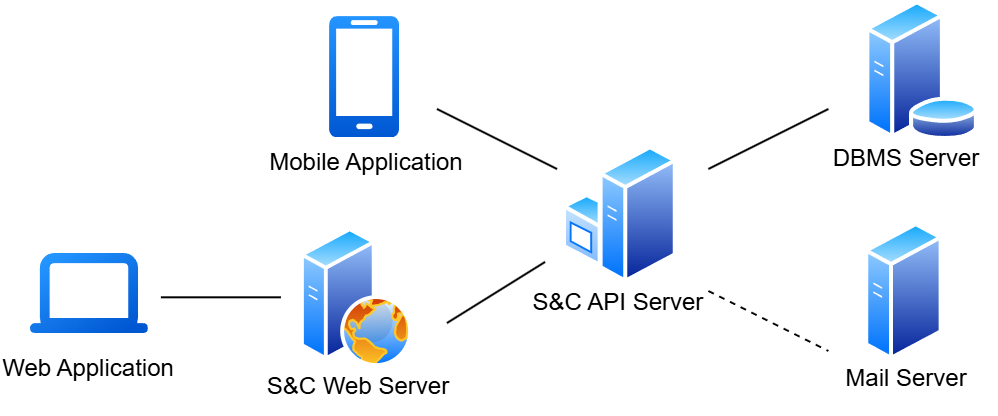
\includegraphics[width=0.9\linewidth]{Images/Architecture design/architecture.png}
    \caption{S\&C architecture overview}
    \label{fig:enter-label}
\end{figure}

The S\&C system is designed using a layered client-server architecture. The system is structured into distinct components, each responsible for specific functionalities such as user management, internship matching, notification handling, and feedback processing. Communication between these components is facilitated through RESTful APIs. This architecture ensures modularity, scalability, and ease of maintenance, allowing for efficient handling of user interactions and system operations.

Client side: 
\begin{itemize}
    \item \textbf{Web Application}: serves as the primary user interface for accessing the S\&C platform. It allows all users (students, companies, and universities) to connect to the system and perform essential operations such as registration, login, and profile management. Through the WebApp, students can search for available internships, apply for them, and track the status of their applications and active internship. Companies can create, update, and manage internship offers, while universities can monitor internship statuses and handle complaints or issues raised during internship. The platform also allows users to create or modify their profiles, including CVs and skills, and manage preferences for internship notifications. The WebApp is designed to be responsive and accessible from any modern browser, offering a smooth experience on both desktop and mobile devices.
    \item \textbf{Mobile Application}: provides a dedicated and optimized version of the S\&C platform for mobile users. It is designed to offer a seamless and intuitive experience for users on the go. Students can easily search for and apply to internships, receive push notifications about new internship offers or application updates, and monitor the status of their applications. Companies can also use the mobile application to create and manage internship offers; however, for tasks that require detailed data entry or management, the desktop version is more convenient and suitable for their needs. In contrast, the mobile application is primarily designed for students who require quick access to the platform’s functionalities. The mobile app supports real-time notifications and is available on both iOS and Android, ensuring accessibility and connectivity for all users.
\end{itemize}
Server side:
\begin{itemize}
    \item \textbf{Web Server}: manages communication with users by receiving and processing their requests. It acts as the gateway between the user and the system, ensuring that all incoming requests are appropriately handled. Additionally, it performs load balancing, distributing incoming traffic across multiple replicas of the S\&C Server to ensure scalability and high availability. The Web Server also handles user sessions, ensuring that users' activities are properly tracked and maintained throughout their interaction with the platform.
    \item \textbf{S\&C API Server}:  is the core component of the system, responsible for processing all requests and managing the primary business functionalities. It hosts the components that handle specific tasks such as user management, internship offers, matchmaking, notifications, and feedback processing. The server acts as the central point of communication between the client applications and the DBMS. All client requests (from the WebApp and Mobile Application) are routed to the appropriate component through a centralized API Gateway, which manages request routing, authentication, and load balancing. To ensure reliability, scalability, and high availability, this Server is deployed across multiple machines or containers. Communication between components can be handled via RESTful APIs for synchronous operations or message brokers (e.g., Apache Kafka) for asynchronous tasks.
    \item \textbf{DBMS Server}: stores all persistent data related to users, students, companies, internships, and interactions within the system. It acts as the primary repository for critical system information, including user profiles, internship offers, applications, feedback, and complaints. The DBMS Server is designed for data integrity, consistency, and quick retrieval of large datasets. It is optimized for performance and supports complex queries needed for matchmaking, reporting, and analytics.
\end{itemize}

\section{Component View}
\label{sec:component_view}
This section presents a detailed breakdown of the components in the system, including their responsibilities, interfaces, and interactions.

\subsection{Component Diagram}
\label{sec:component_diagram}
\begin{figure}[H]
    \centering
    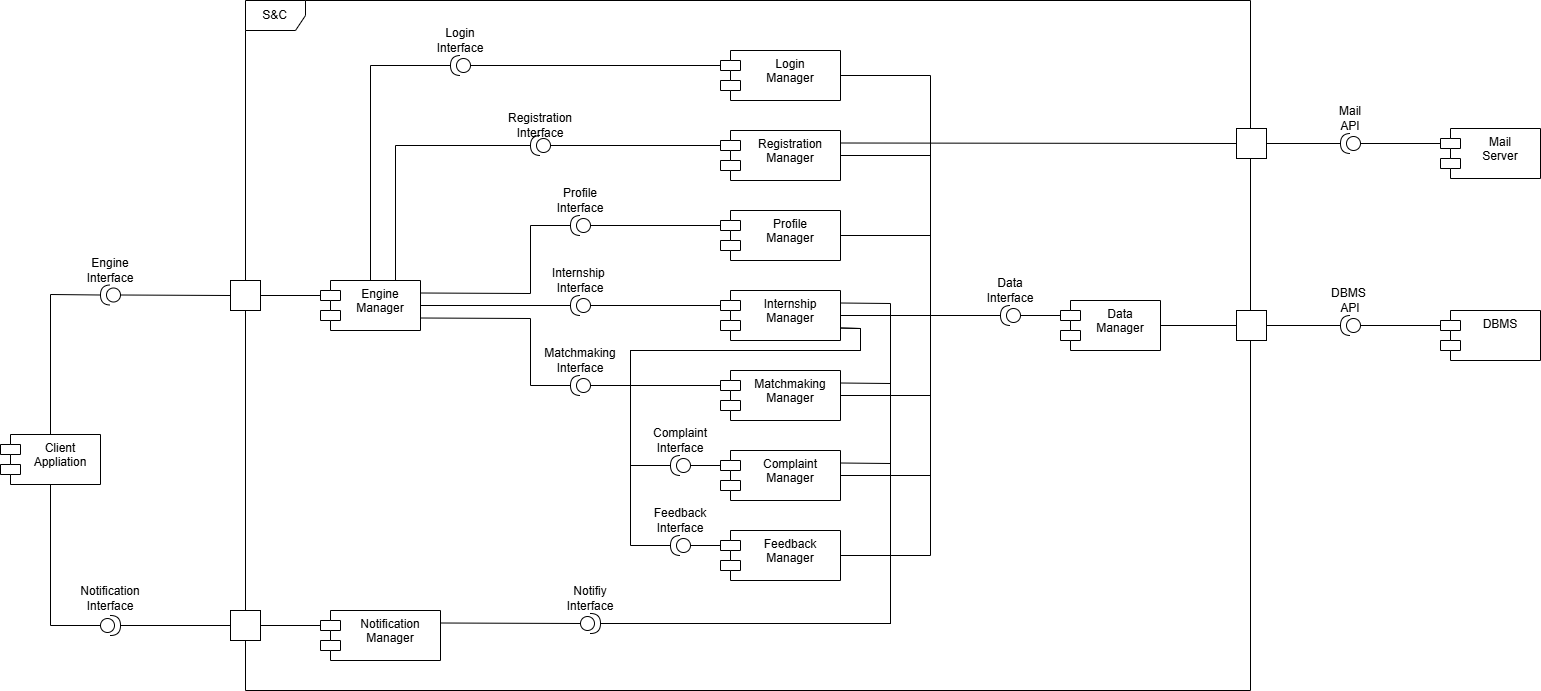
\includegraphics[width=1\linewidth]{Images/Component diagrams/ComponentDiagram.png}
    \caption{S\&C component diagram }
    \label{fig:enter-label}
\end{figure}

\subsection{Components Description}
\label{sec:component_diagram}
The components are:
\begin{itemize}
    \item \textbf{Client Application}: is the central access point for users to interact with the system. It provides the user interface through which users can perform key actions, such as logging into their accounts, registering as new users, managing personal information, submitting feedback, and accessing internship opportunities. The Client Application acts as the bridge between the user and the underlying services, sending requests to appropriate components and receiving responses to display the necessary information to the user.
    \item \textbf{Engine Manager}: serves as the core orchestration component within the system. It receives and processes user requests originating from the Client Application and coordinates the execution of these tasks by delegating them to appropriate services, such as the Login Manager, Internship Manager, or Notification Manager. By managing inter-component communication, the Engine Manager ensures the system operates efficiently and cohesively.
    \item \textbf{Login Manager}: handles the entire user authentication process. It verifies credentials provided during the login attempt by querying the DBMS to check for valid user data. If the credentials match, the Login Manager grants access to the system, ensuring that only authorized users can interact with protected services. It also manages failed login attempts, providing appropriate feedback to the user.

    \begin{figure}[H]
        \centering
        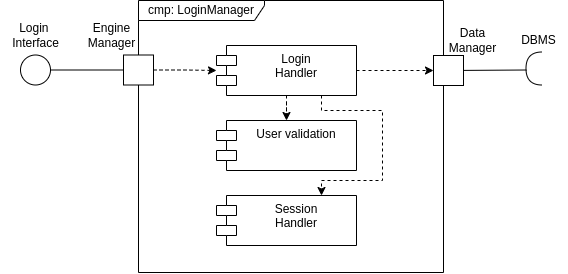
\includegraphics[width=0.9\linewidth]{Images/Component diagrams/ComponentDiagram_Login.png}
        \caption{Login manager component diagram}
        \label{fig:enter-label}
    \end{figure}
    
    \item \textbf{Registration Manager}: oversees the user registration process, enabling new users to create accounts within the system. It validates user-provided input (e.g., name, email, password) and securely communicates with the DBMS to store new account details. Additionally, it can trigger email confirmations through the Mail Server to verify user identities and ensure secure onboarding.

    \begin{figure}[H]
        \centering
        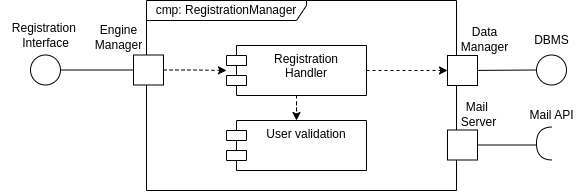
\includegraphics[width=0.9\linewidth]{Images/Component diagrams/ComponentDiagram_Registration.png}
        \caption{Registration manager component diagram}
        \label{fig:enter-label}
    \end{figure}
    
    \item \textbf{Profile Manager}: is responsible for handling all operations related to user profiles. It allows users to retrieve, view, and update personal data such as contact details, resumes, or preferences. This component ensures the integrity of profile updates by interacting directly with the DBMS to persist changes. It acts as a crucial service for maintaining user data consistency across the platform.

    \begin{figure}[H]
        \centering
        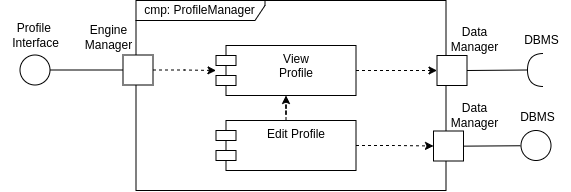
\includegraphics[width=0.9\linewidth]{Images/Component diagrams/ComponentDiagram_Profile.png}
        \caption{Profile manager component diagram}
        \label{fig:enter-label}
    \end{figure}
    
    \item \textbf{Internship Manager}: manages all operations related to internship opportunities. It allows system administrators to create, update, and delete internship postings while enabling users to search for and apply to available positions. It interacts with the DBMS to persist internship data, including details like job descriptions, requirements, and application deadlines. This service ensures up-to-date internship information is always available to users.

    \begin{figure}[H]
        \centering
        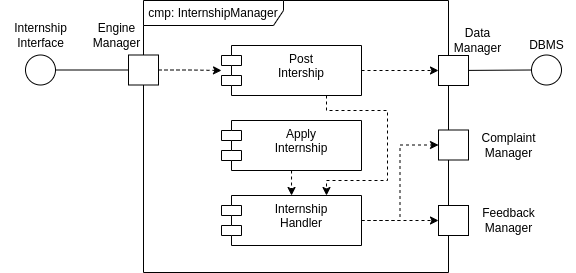
\includegraphics[width=0.9\linewidth]{Images/Component diagrams/ComponentDiagram_Internship.png}
        \caption{Internship manager component diagram}
        \label{fig:enter-label}
    \end{figure}
    
    \item \textbf{Matchmaking Manager}: is a specialized component that aligns user profiles with suitable internship opportunities. It leverages user data—such as resumes, preferences, and skills—and compares it with internship requirements stored in the DBMS. By running matching algorithms, it identifies relevant opportunities for users and generates recommendations, streamlining the search process for internships.
    \item \textbf{Complaint Manager}: allows users to report issues, concerns, or grievances within the system. It provides a structured mechanism to log complaints, which are stored in the DBMS for review and resolution by administrators. The Complaint Manager ensures that user-reported problems are tracked and appropriately addressed to improve overall user satisfaction.

    \begin{figure}[H]
        \centering
        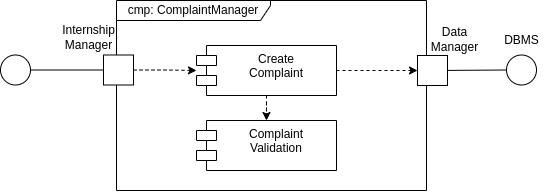
\includegraphics[width=0.9\linewidth]{Images/Component diagrams/ComponentDiagram_Complaint.png}
        \caption{Complaint manager component diagram}
        \label{fig:enter-label}
    \end{figure}
    
    \item \textbf{Feedback Manager}: is responsible for collecting and managing feedback submitted by users. It allows users to share their experiences or provide evaluations of system services. The component interacts with the DBMS to store feedback, which can later be analyzed to identify areas for improvement. This ensures continuous enhancement of the system based on user input.

    \begin{figure}[H]
        \centering
        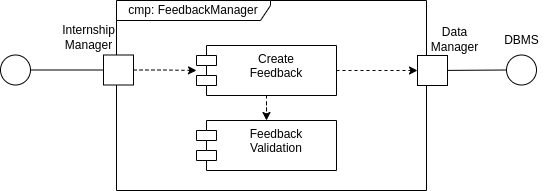
\includegraphics[width=0.9\linewidth]{Images/Component diagrams/ComponentDiagram_Feedback.png}
        \caption{Feedback manager component diagram}
        \label{fig:enter-label}
    \end{figure}
    
    \item \textbf{Notification Manager}: handles the delivery of system notifications to users. It processes requests from other components, such as the Engine Manager or Complaint Manager, to notify users about updates, events, or critical actions requiring attention. Notifications can be sent via in-app messages or through integration with the Mail Server for email delivery. This component ensures users remain up to date with relevant information.
    \item \textbf{Data Manager}: acts as the intermediary layer responsible for managing communication between components and the DBMS. It handles data retrieval, insertion, and updates, ensuring that services have seamless access to accurate and consistent data. The Data Manager ensures the integrity and security of the system’s database operations, facilitating efficient data management.
    \item \textbf{DBMS}: serves as the centralized data repository for the system. It stores all essential information, including user credentials, profiles, internship postings, complaints, and feedback. The DBMS ensures data persistence, consistency, and availability, enabling components to query and update data as needed. It forms the backbone of the system's data management architecture.
\end{itemize}

% Add the description of each component here.

\section{Deployment View}
\label{sec:deployment_view}
The deployment view describes how the system is physically deployed and the interactions between its components.
\begin{figure}[H]
    \centering
    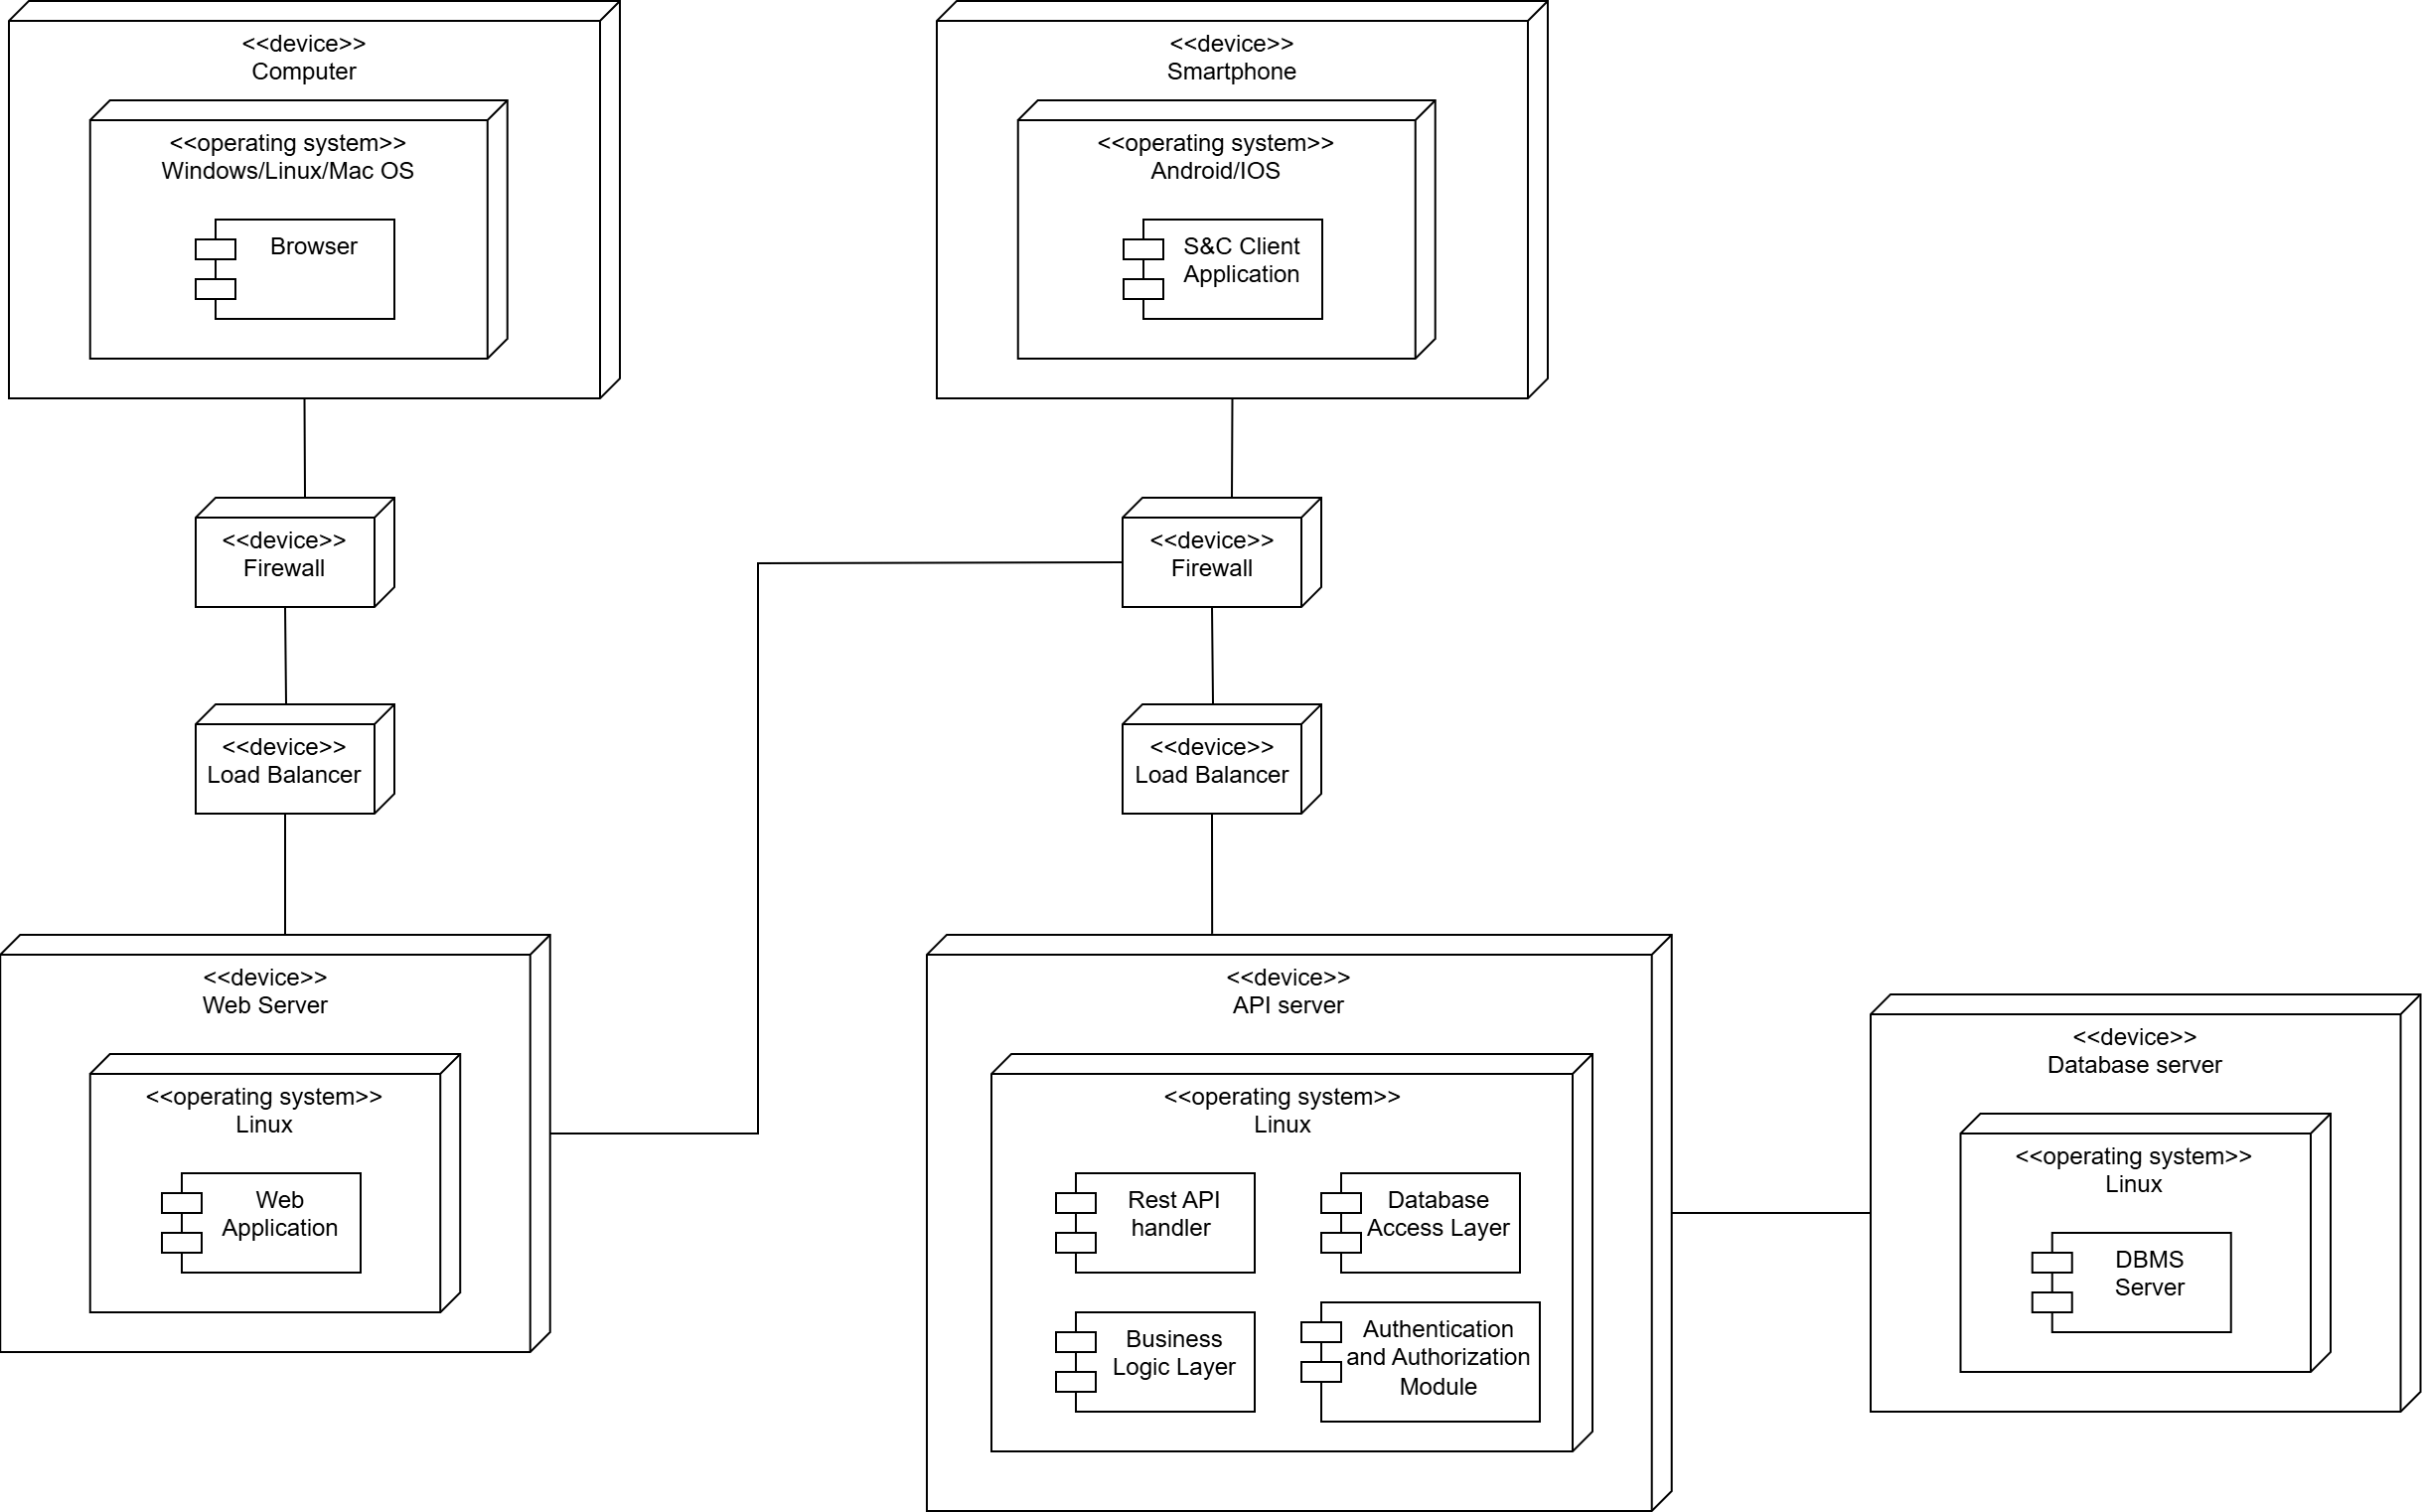
\includegraphics[width=1\linewidth]{Images/Deployment diagram/deploymentView.png}
    \caption{Deployment view diagram}
    \label{fig:enter-label}
\end{figure}

\textbf{Client Devices} \\
The system supports two types of client devices:
\begin{itemize}
    \item Computers: users can access the system via browsers on devices running different operating systems. The browser-based interface ensures cross-platform compatibility and ease of access.
    \item Smartphones: Users on Android or iOS can interact with the system through a dedicated S\&C Client Application, offering a mobile-friendly experience with tailored functionalities.
\end{itemize}

\textbf{Firewall} \\
The communication between the client devices and the backbend system is safeguarded by a Firewall. It filters incoming and outgoing traffic, protecting the system from unauthorized access, malicious attacks and data breaches.

\textbf{Load Balancer} \\
The Load Balancer is used to maintain system availability and performance by distributing incoming request across multiple backend servers. This ensures that non single server becomes a bottleneck, improving reliability and accommodating high traffic volumes.

\textbf{Web Server} \\
It serves as the entry point for users interacting via browser. It hosts the Web Application which handles the frontend functionality, rendering the user interface and responding to user actions and session management, maintaining session continuity for user logged in via web browsers.
\textbf{API Server} \\
The S\&C API Server is the heart of the system's backend logic. It is composed by several key components:
\begin{itemize}
    \item Rest API Handler: acts as the communication bridge between client requests and backend logic, ensuring proper routing and handling of API calls.
    \item Business Logic Layer: implements the core system functionalities such as processing user actions, handling workflows and executing business rules.
    \item Database Access Layer: provides a secure and optimized interface for querying and updating data in the database server.
    \item Authentication and Authorization Module: enforces user authentication and role-based permissiones to protect sensistive operations and data.
\end{itemize}

\textbf{Database server} \\
The Database server manages the system's data using a DBMS.

\section{Runtime View}
\label{sec:runtime_view}
In this section, S\&C system are presented through sequence diagrams. Initially, the actions of the S\&C system are shown from the perspective of the student user, such as logging in, applying for internships, updating their profile, and managing their preferences. Then, the actions are presented from the perspective of the company user, which involve more business-oriented functionalities, such as managing internship offers, reviewing applications, and scheduling interviews. Finally, university ones, such as the internship interruption.

\newcounter{uc}
\setcounter{uc}{1}
\newcommand{\cuc}{\theuc\stepcounter{uc}}

\textbf{UC\cuc\  - User registration} \\
The figure shows the registration process for students and companies. Once the request is sent it will automatically start the process of authentication which is managed by the Registration manager. The process continues with the student/company filling in the necessary information in order to successfully create the users profile. As soon as the form is submitted and sent to the registration manager, the database is checked to control whether another user with the same information already exists on the platform. If there is no user with the same credentials then a new user is created and added to the corresponding table.
\begin{center}
    \begin{figure}[H]
        \centering
        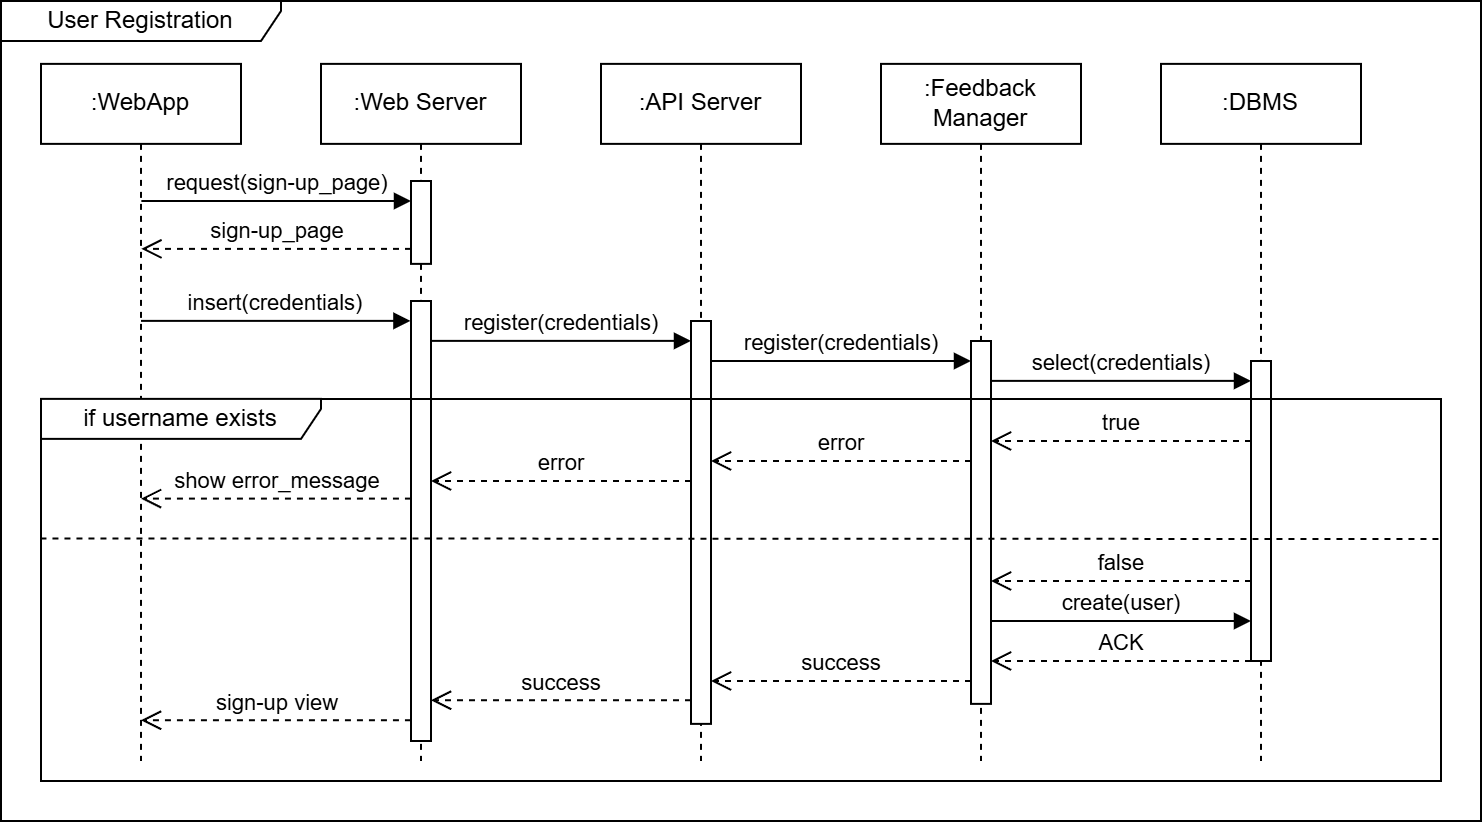
\includegraphics[width=1\linewidth]{Images/Sequence diagrams/UC1.png}
        \caption{Student Registration}
        \label{fig:enter-label}
    \end{figure}
\end{center}

\textbf{UC\cuc\  - User, student, company or university login} \\
The figure shows the process of a user login. Even if the information of every user has been stored in a separate database, one for each type of user, the process is the same.
\begin{center}
    \begin{figure}[H]
        \centering
        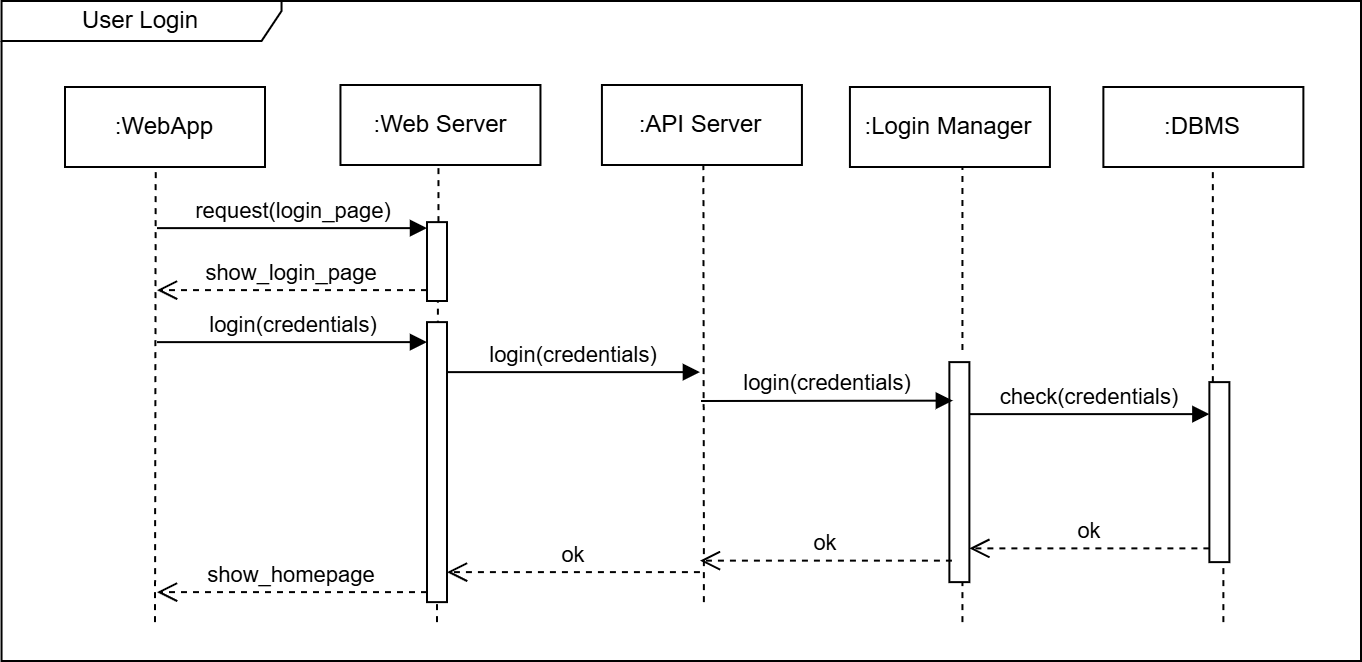
\includegraphics[width=1\linewidth]{Images/Sequence diagrams/UC2.png}
        \caption{User Login}
        \label{fig:enter-label}
    \end{figure}
\end{center}
    

\textbf{UC\cuc\  - Student’s account activation} \\
The figure shows the process of upgrading an account from standard registered user to a verified students account. After inserting the additional details required to do the upgrade correctly and after checking that there are no other students with the same credentials the Notification manager proceeds to send an email containing a verification link that the student must press in order to confirm the upgrade.
\begin{center}
    \begin{figure}[H]
        \centering
        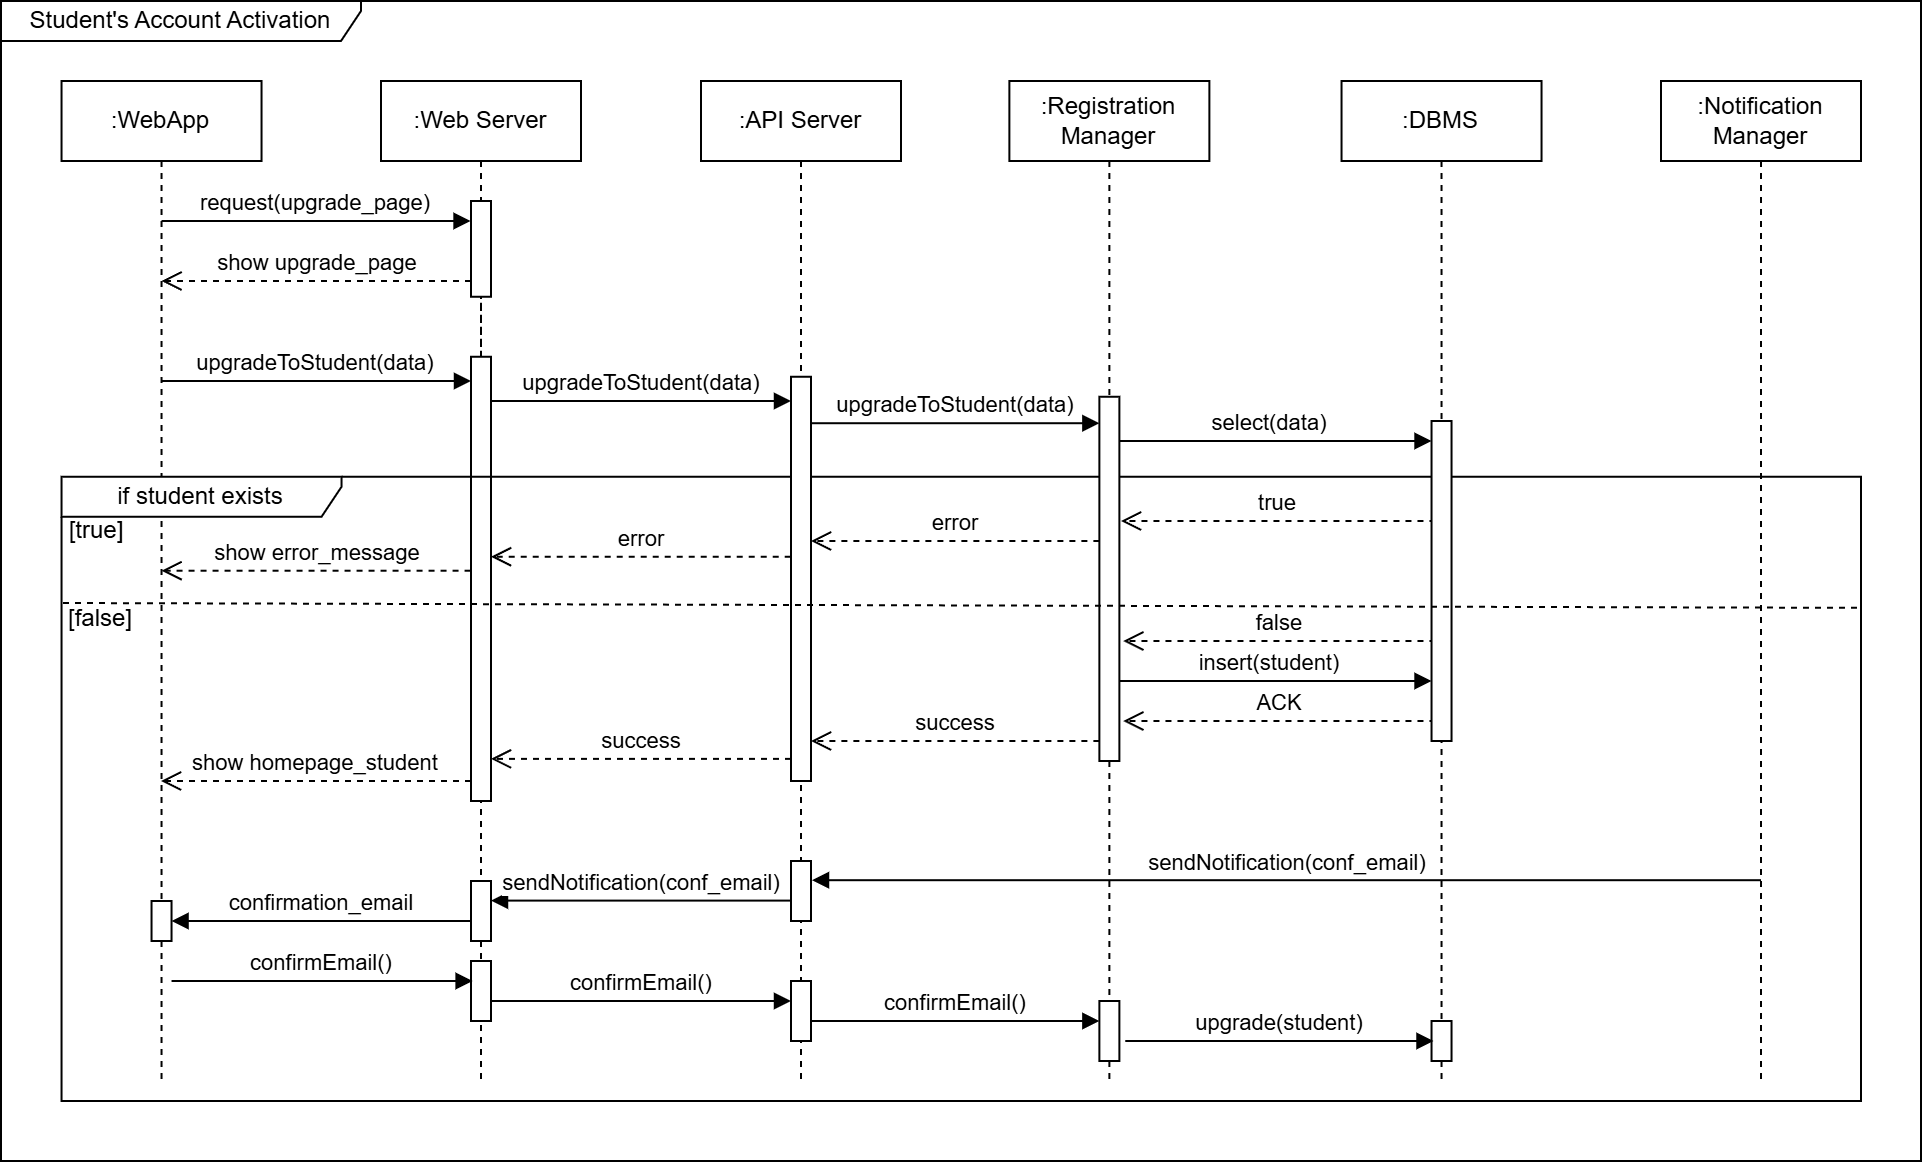
\includegraphics[width=1\linewidth]{Images/Sequence diagrams/UC3.png}
        \caption{Student's Account Activation}
        \label{fig:enter-label}
    \end{figure}
\end{center}


\textbf{UC\cuc\  - Student modifies their profile or updates their CV} \\
The diagram outlines the process for updating a student's profile. The WebApp sends requests to the Web Server and forwards them to the API Server. For CV updates or personal data changes, the Profile Manager processes the requests and updates the DBMS. Success or error messages are sent back to the WebApp for display.
\begin{center}
    \begin{figure}[H]
        \centering
        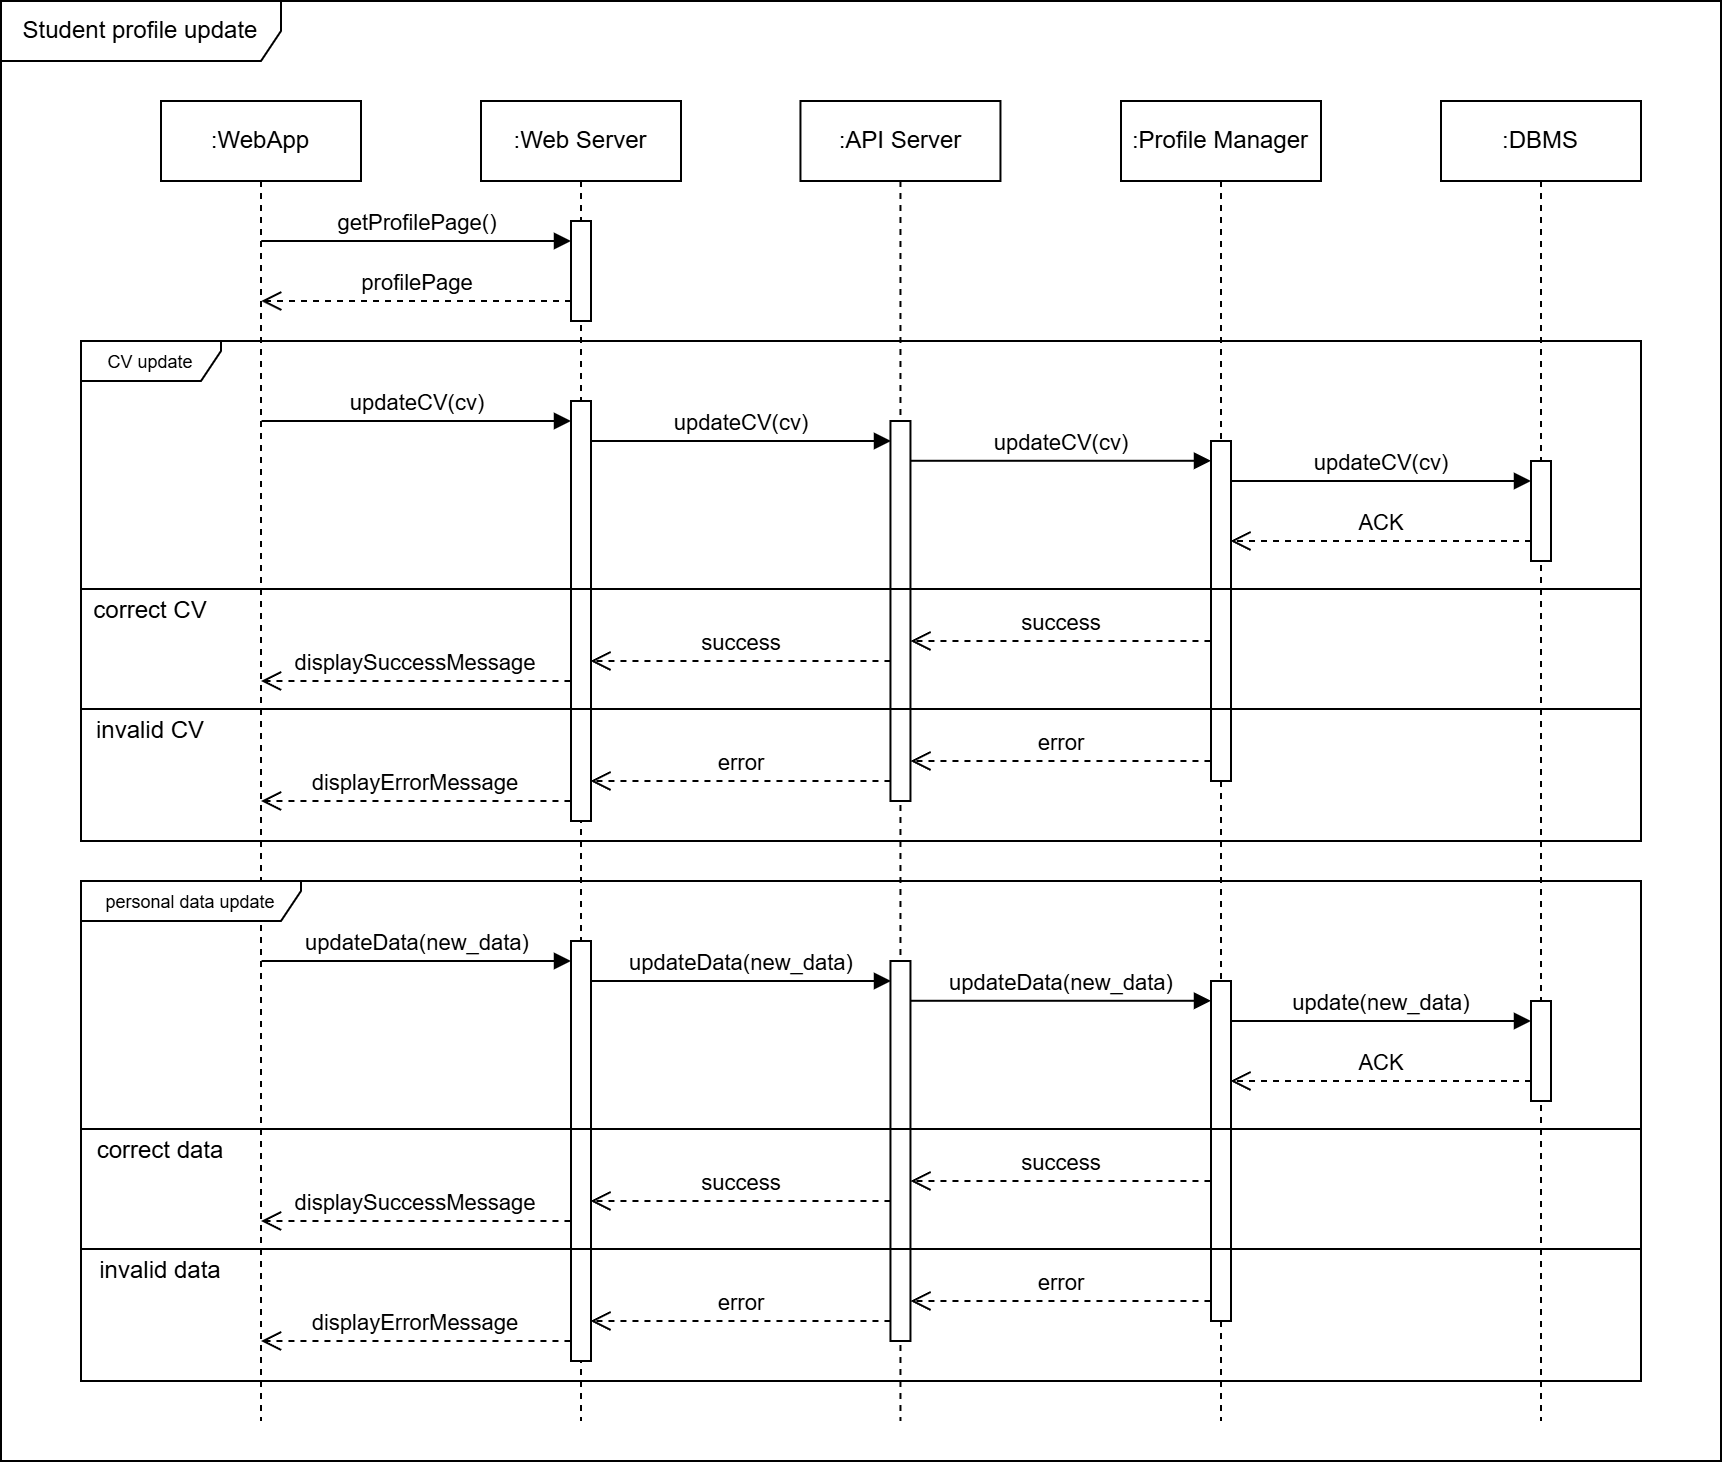
\includegraphics[width=1\linewidth]{Images/Sequence diagrams/UC4.png}
        \caption{Student's Profile Update}
        \label{fig:enter-label}
    \end{figure}
\end{center}

\textbf{UC\cuc\ - UC\cuc\ - UC\cuc\  - Student checks available offers, opens the details page of an internship post, and sends an application for it} \\
The diagram shows the application process for internships. The WebApp requests internship details through the Web Server, which retrieves them via the API Server from the Internship Manager and DBMS. After reviewing, the student sends an application, which is processed and stored. Feedback on success or errors is then displayed to the student.
\begin{center}
    \begin{figure}[H]
        \centering
        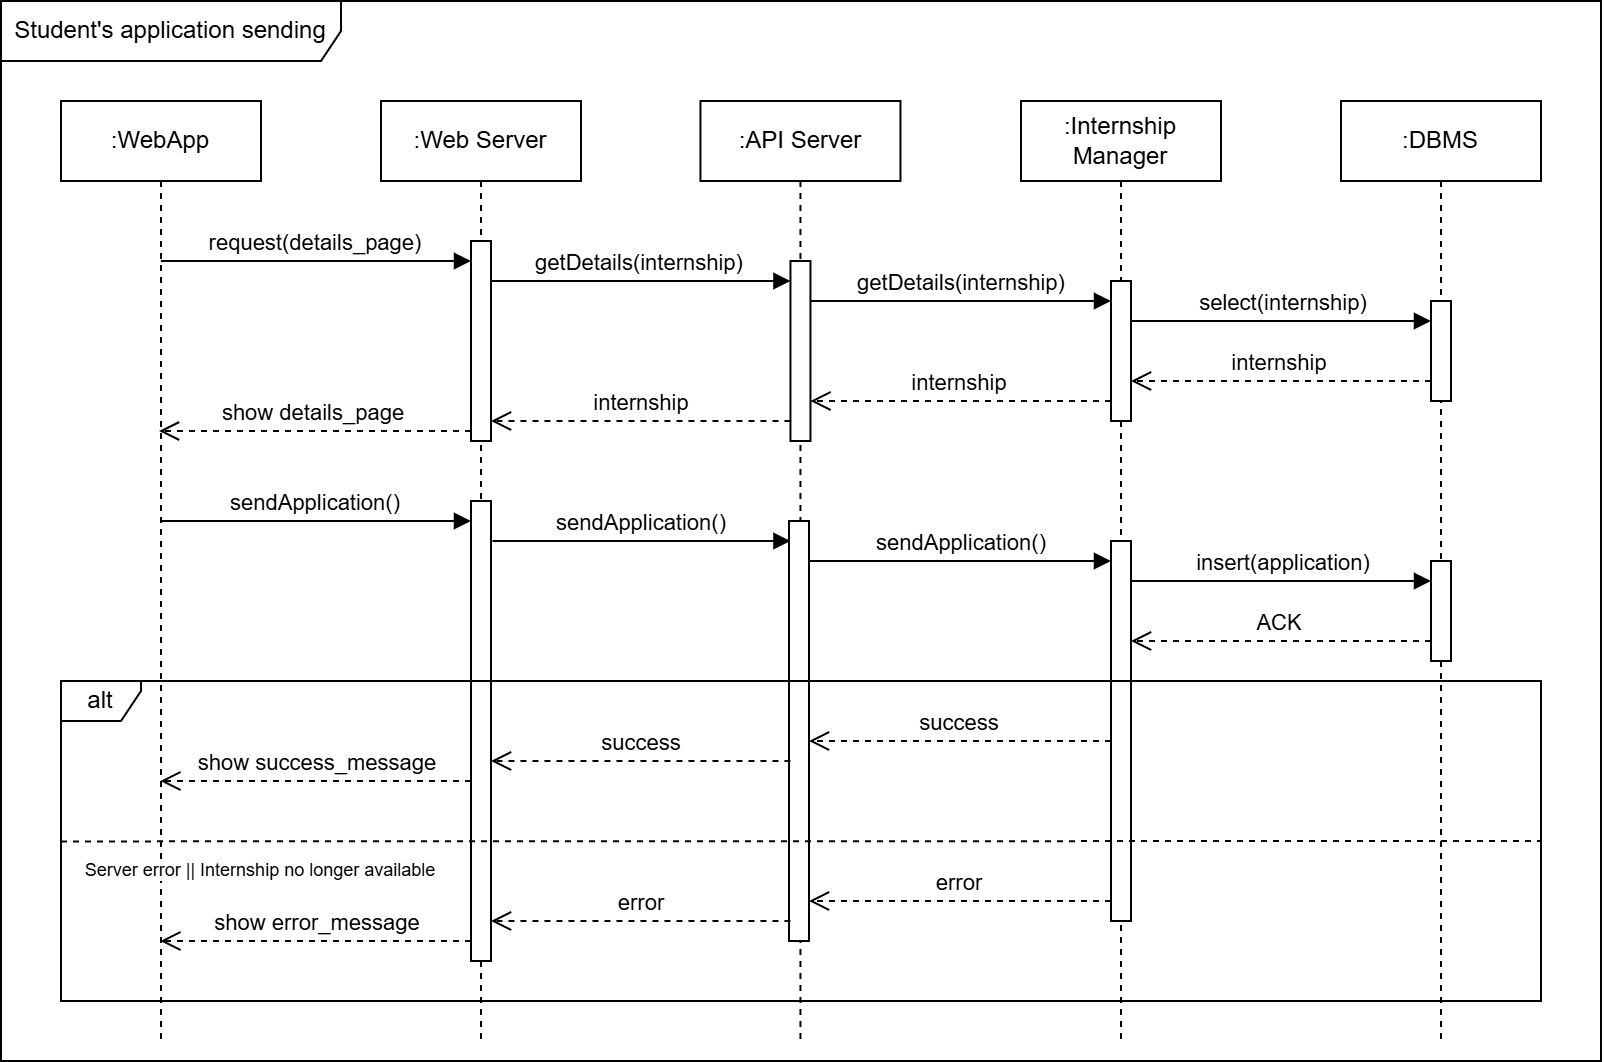
\includegraphics[width=1\linewidth]{Images/Sequence diagrams/UC567.png}
        \caption{Student's Application sending Update}
        \label{fig:enter-label}
    \end{figure}
\end{center}

\textbf{UC\cuc\ - Student accepts or denies an interview schedule proposal from the company} \\
The diagram illustrates the process for a student's schedule response. Notifications are sent from the Internship Manager through the API Server to the WebApp. The student can either accept or reject the schedule. The respective action triggers an action, processed by the Internship Manager and reflected in the DBMS. A confirmation message is then displayed to the student on the WebApp.
\begin{center}
    \begin{figure}[H]
        \centering
        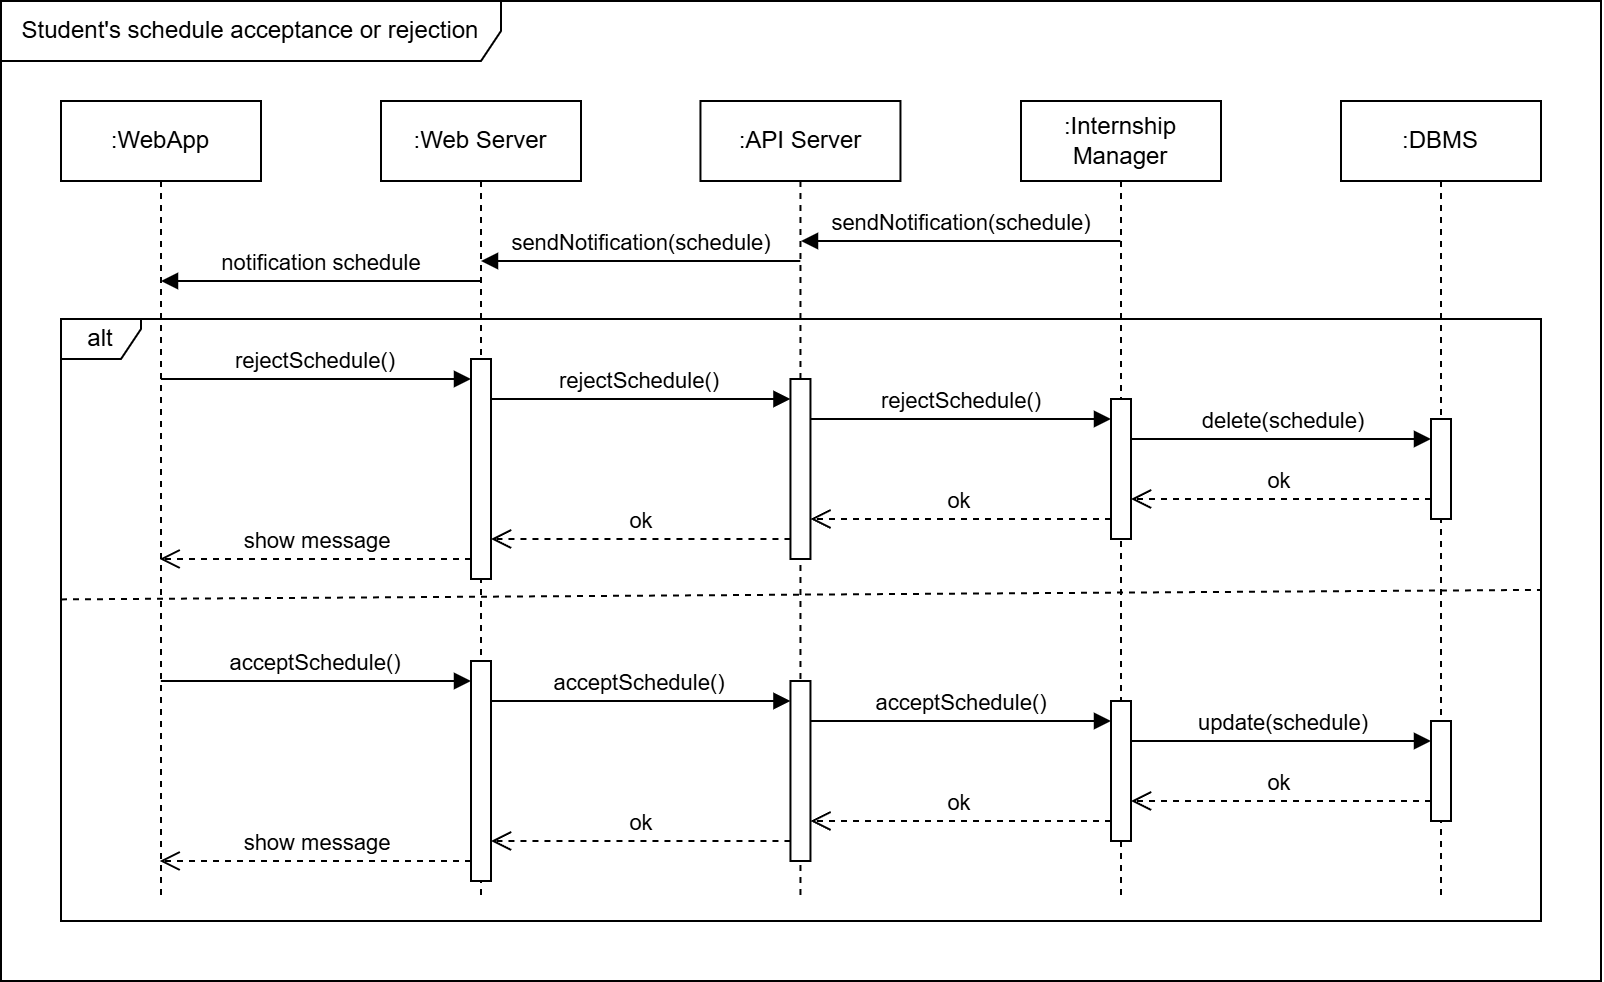
\includegraphics[width=1\linewidth]{Images/Sequence diagrams/UC8.png}
        \caption{Student's Application sending Update}
        \label{fig:enter-label}
    \end{figure}
\end{center}

\textbf{UC\cuc\ - Student accepts or denies the start of the internship} \\
The diagram illustrates the process for the final decision of a student. The student receives a notification to confirm or reject the start of the internship, following the positive decision of the company after the interview. If the student accepts, the confirmation is sent through the Web Server and API Server to the Internship Manager, which updates the database to finalize the start. If the student rejects, a similar process is followed to record the rejection in the database. In both scenarios, a success message is displayed.
\begin{center}
    \begin{figure}[H]
        \centering
        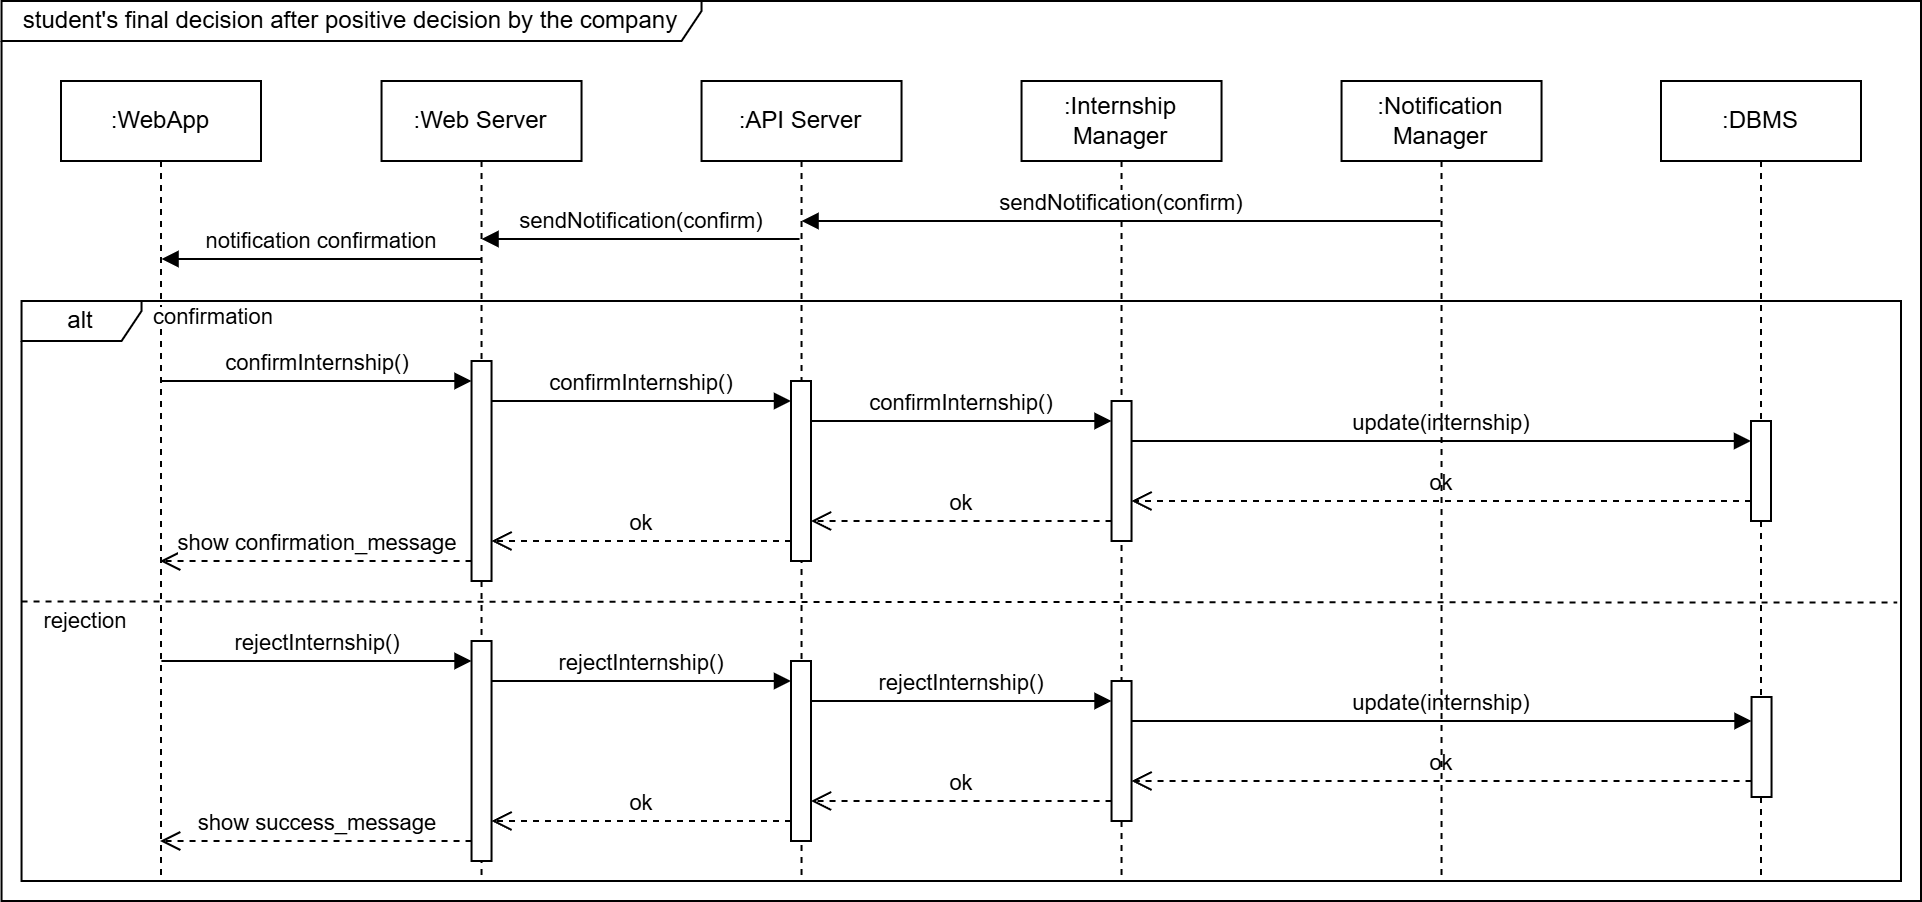
\includegraphics[width=1\linewidth]{Images/Sequence diagrams/UC9.png}
        \caption{Student's Application sending Update}
        \label{fig:enter-label}
    \end{figure}
\end{center}

\textbf{UC\cuc\  - Company’s account activation} \\
The figure shows the process of upgrading an account from standard registered user to a verified company account. The process consists of inserting the additional details required to do the upgrade correctly and checking that there are no other companies with the same credentials.
\begin{center}
    \begin{figure}[H]
        \centering
        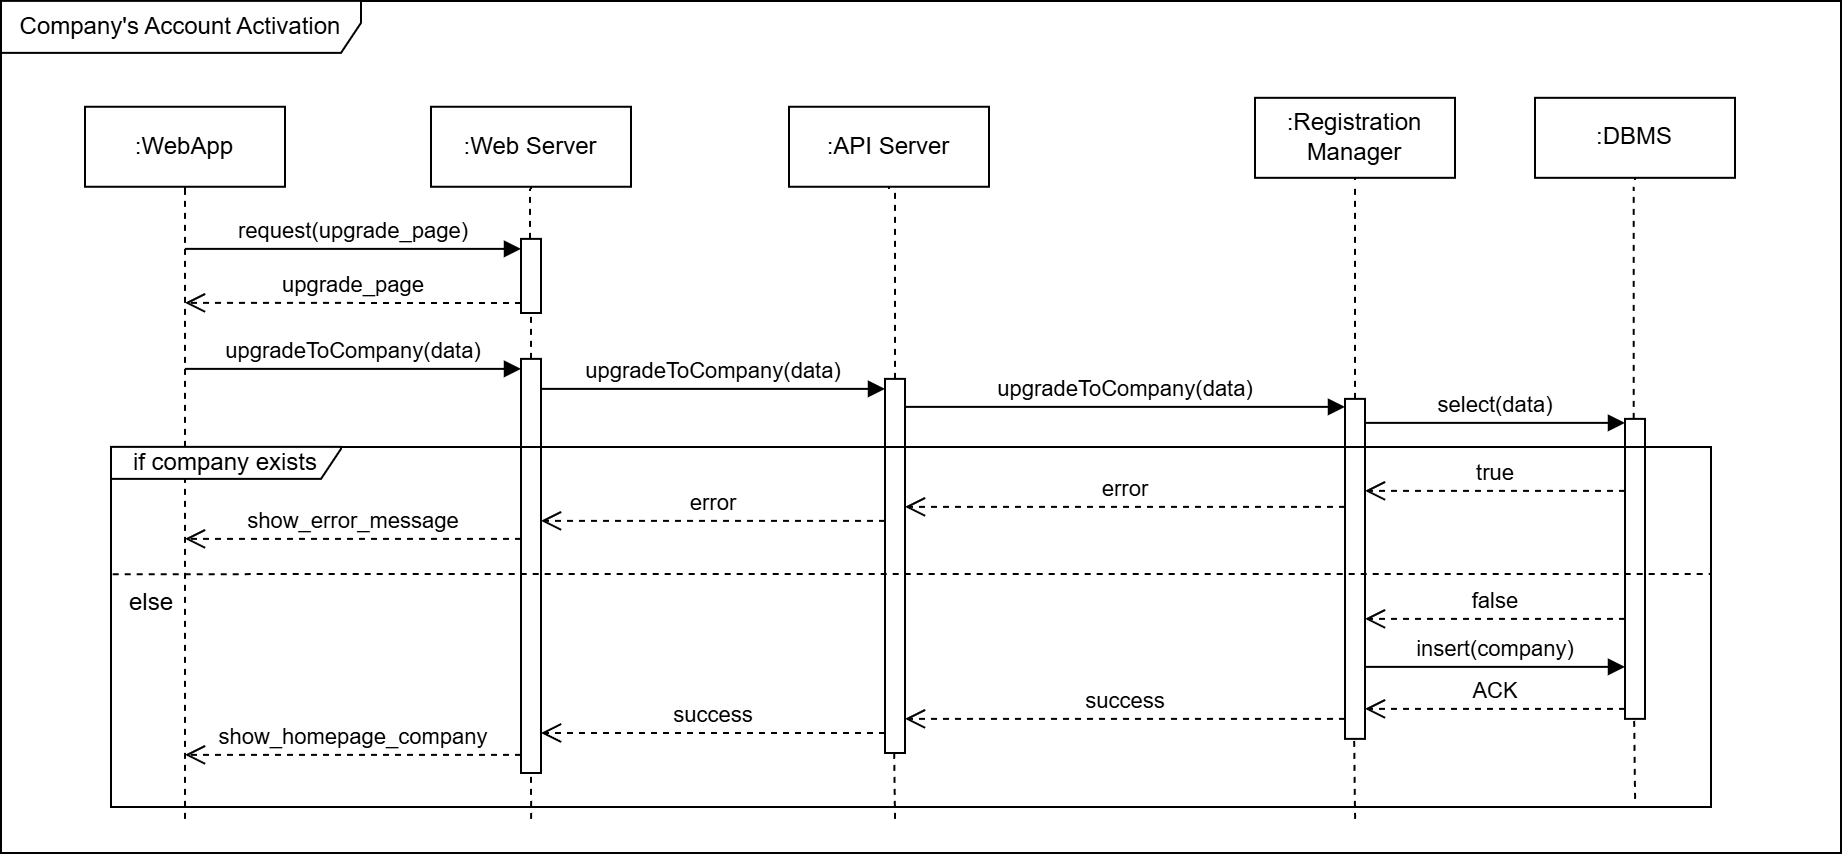
\includegraphics[width=1\linewidth]{Images/Sequence diagrams/UC10.png}
        \caption{Company Account Activation}
        \label{fig:enter-label}
    \end{figure}
\end{center}

\textbf{UC\cuc\  - Company's profile modification} \\
The diagram shows the process for updating a company's profile. The company accesses its profile page to modify its information. After making the desired changes, the updated data are sent through the Web Server and API Server to the Profile Manager. The Profile Manager validates the modifications and updates the database. In case of a successful completion, a confirmation message is displayed to the company. In case of errors, an error message is shown instead.
\begin{center}
    \begin{figure}[H]
        \centering
        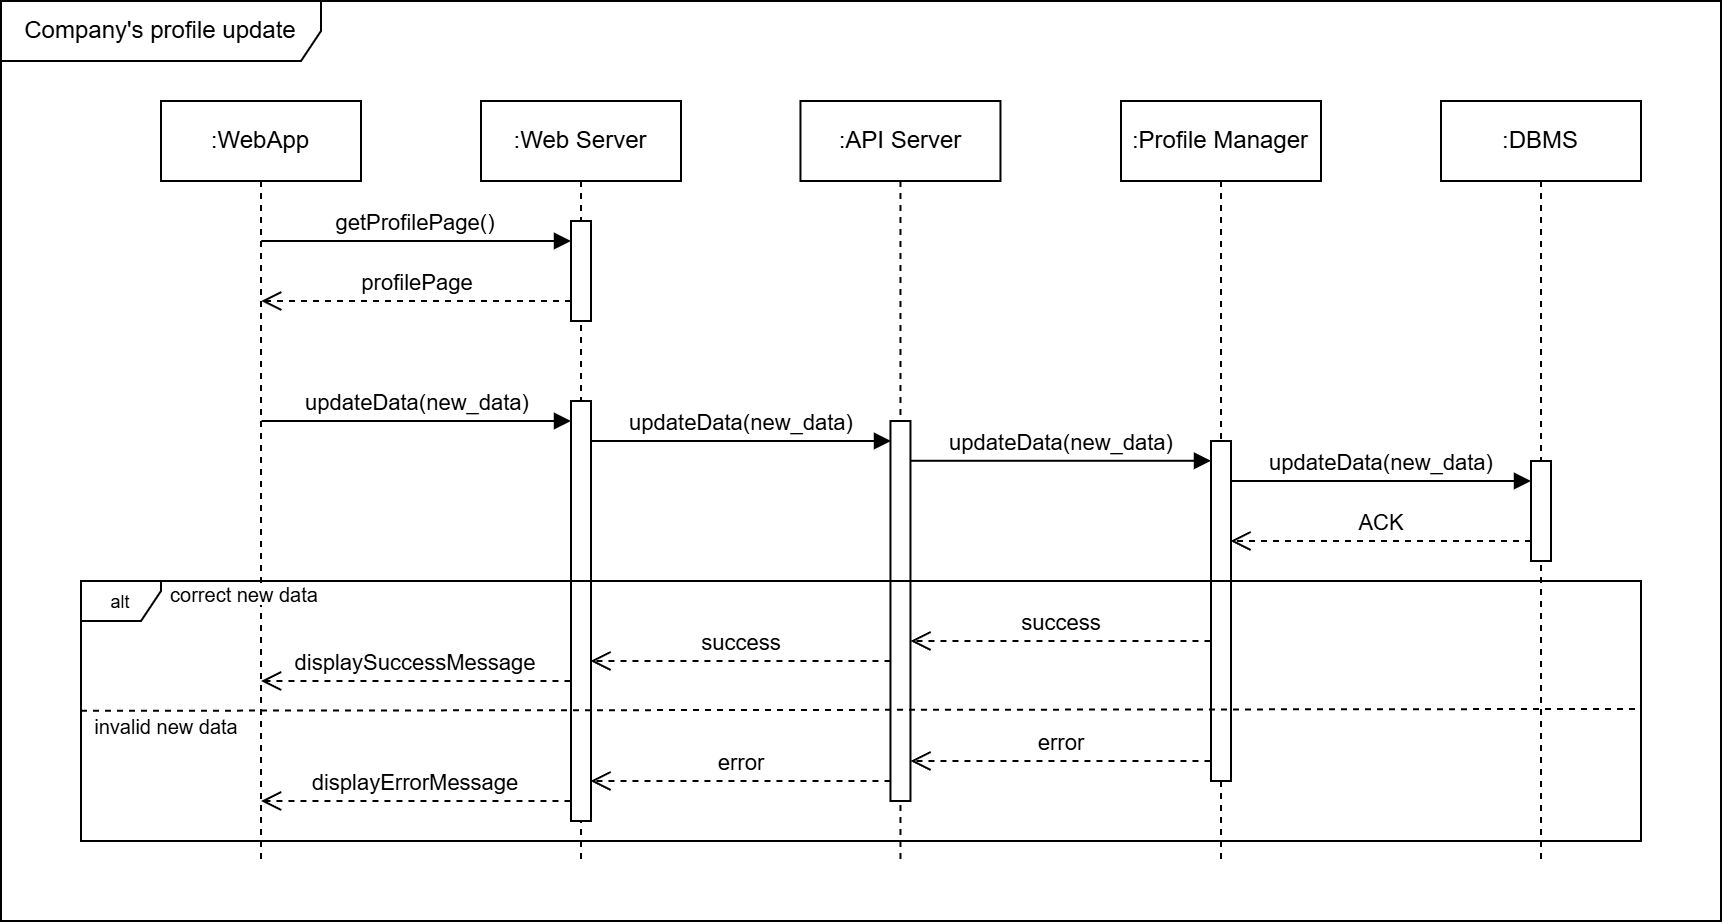
\includegraphics[width=1\linewidth]{Images/Sequence diagrams/UC11.png}
        \caption{Company's Profile Update}
        \label{fig:enter-label}
    \end{figure}
\end{center}

\textbf{UC\cuc\ - Company posts a new internship} \ The figure shows the process of posting a new internship offer by a company. The company accesses the dedicated page with a form, fills in all the fields, and submits the required data. After the request is submitted to the Web Server and API Server, it is forwarded to the Internship Manager. The Internship Manager validates the data and proceeds to insert it into the database. In case of successful completion, a confirmation message is displayed to the company. In case of errors, an error message is shown instead.
\begin{center}
    \begin{figure}[H]
        \centering
        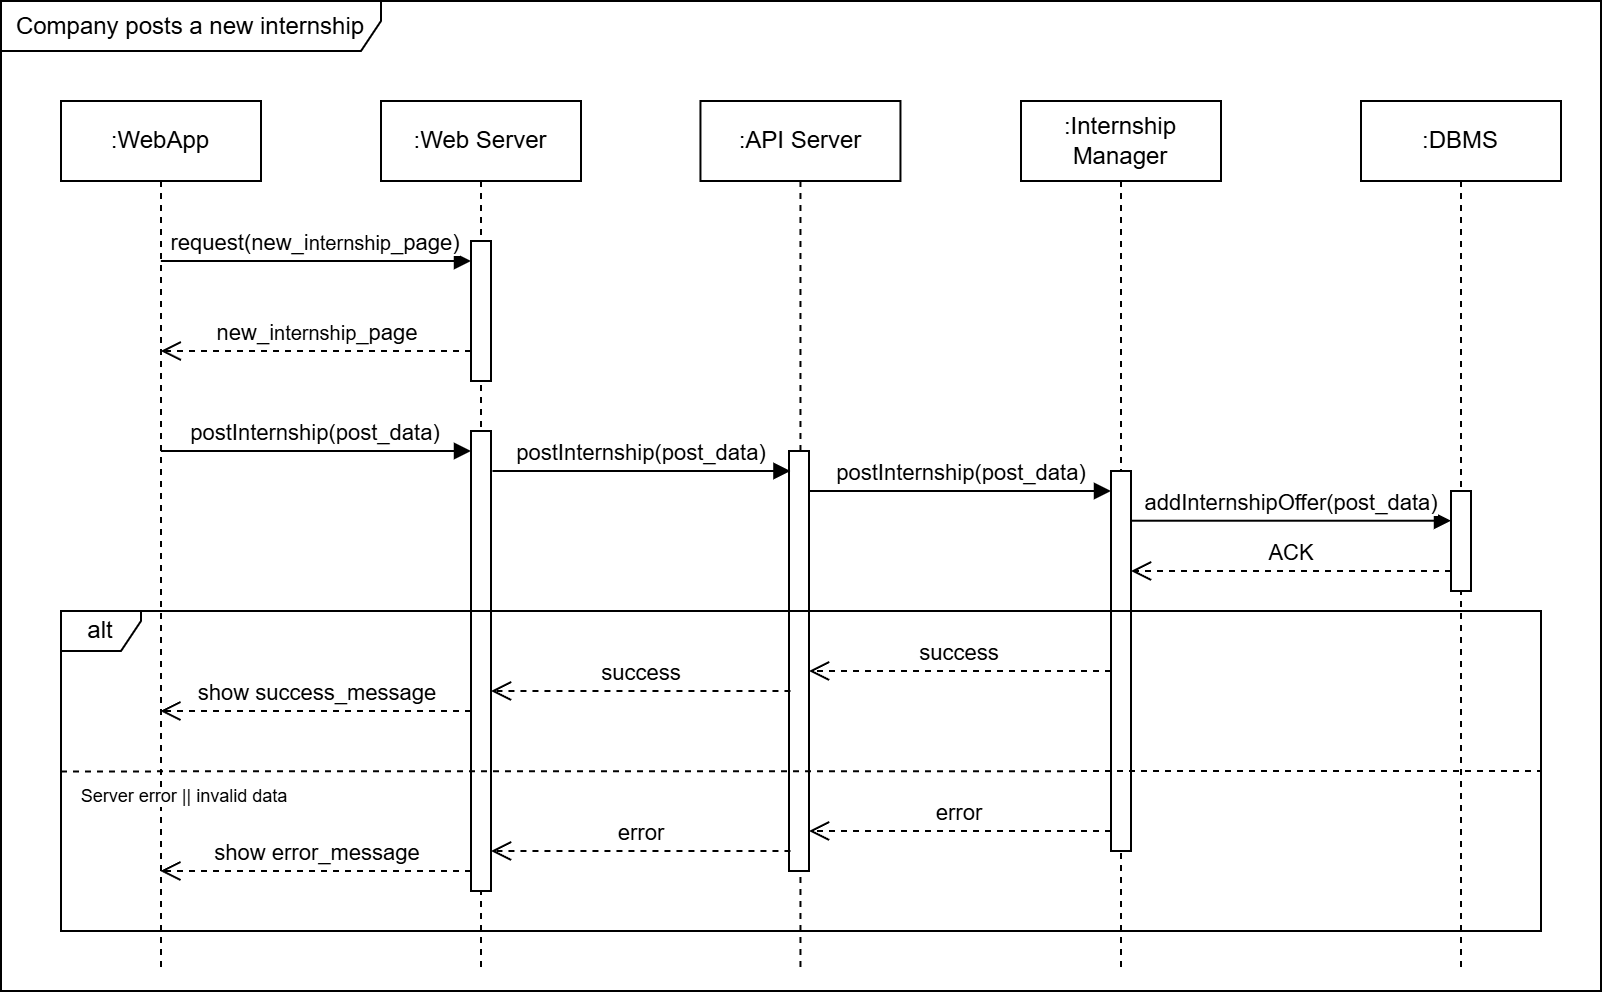
\includegraphics[width=1\linewidth]{Images/Sequence diagrams/UC12.png}
        \caption{Company new offer posting}
        \label{fig:enter-label}
    \end{figure}
\end{center}

\textbf{UC\cuc\  - The company accepts an application or identifies a promising student and
proposes a schedule for the interview} \\
The diagram illustrates the process where a company selects candidates for an internship, views a student's details, and proposes a schedule. The WebApp communicates with the Web Server, API Server, and respective managers (Matchmaking, Profile, Internship) to retrieve data and submit the schedule. Success or error messages are displayed based on the operation outcome.
\begin{center}
    \begin{figure}[H]
        \centering
        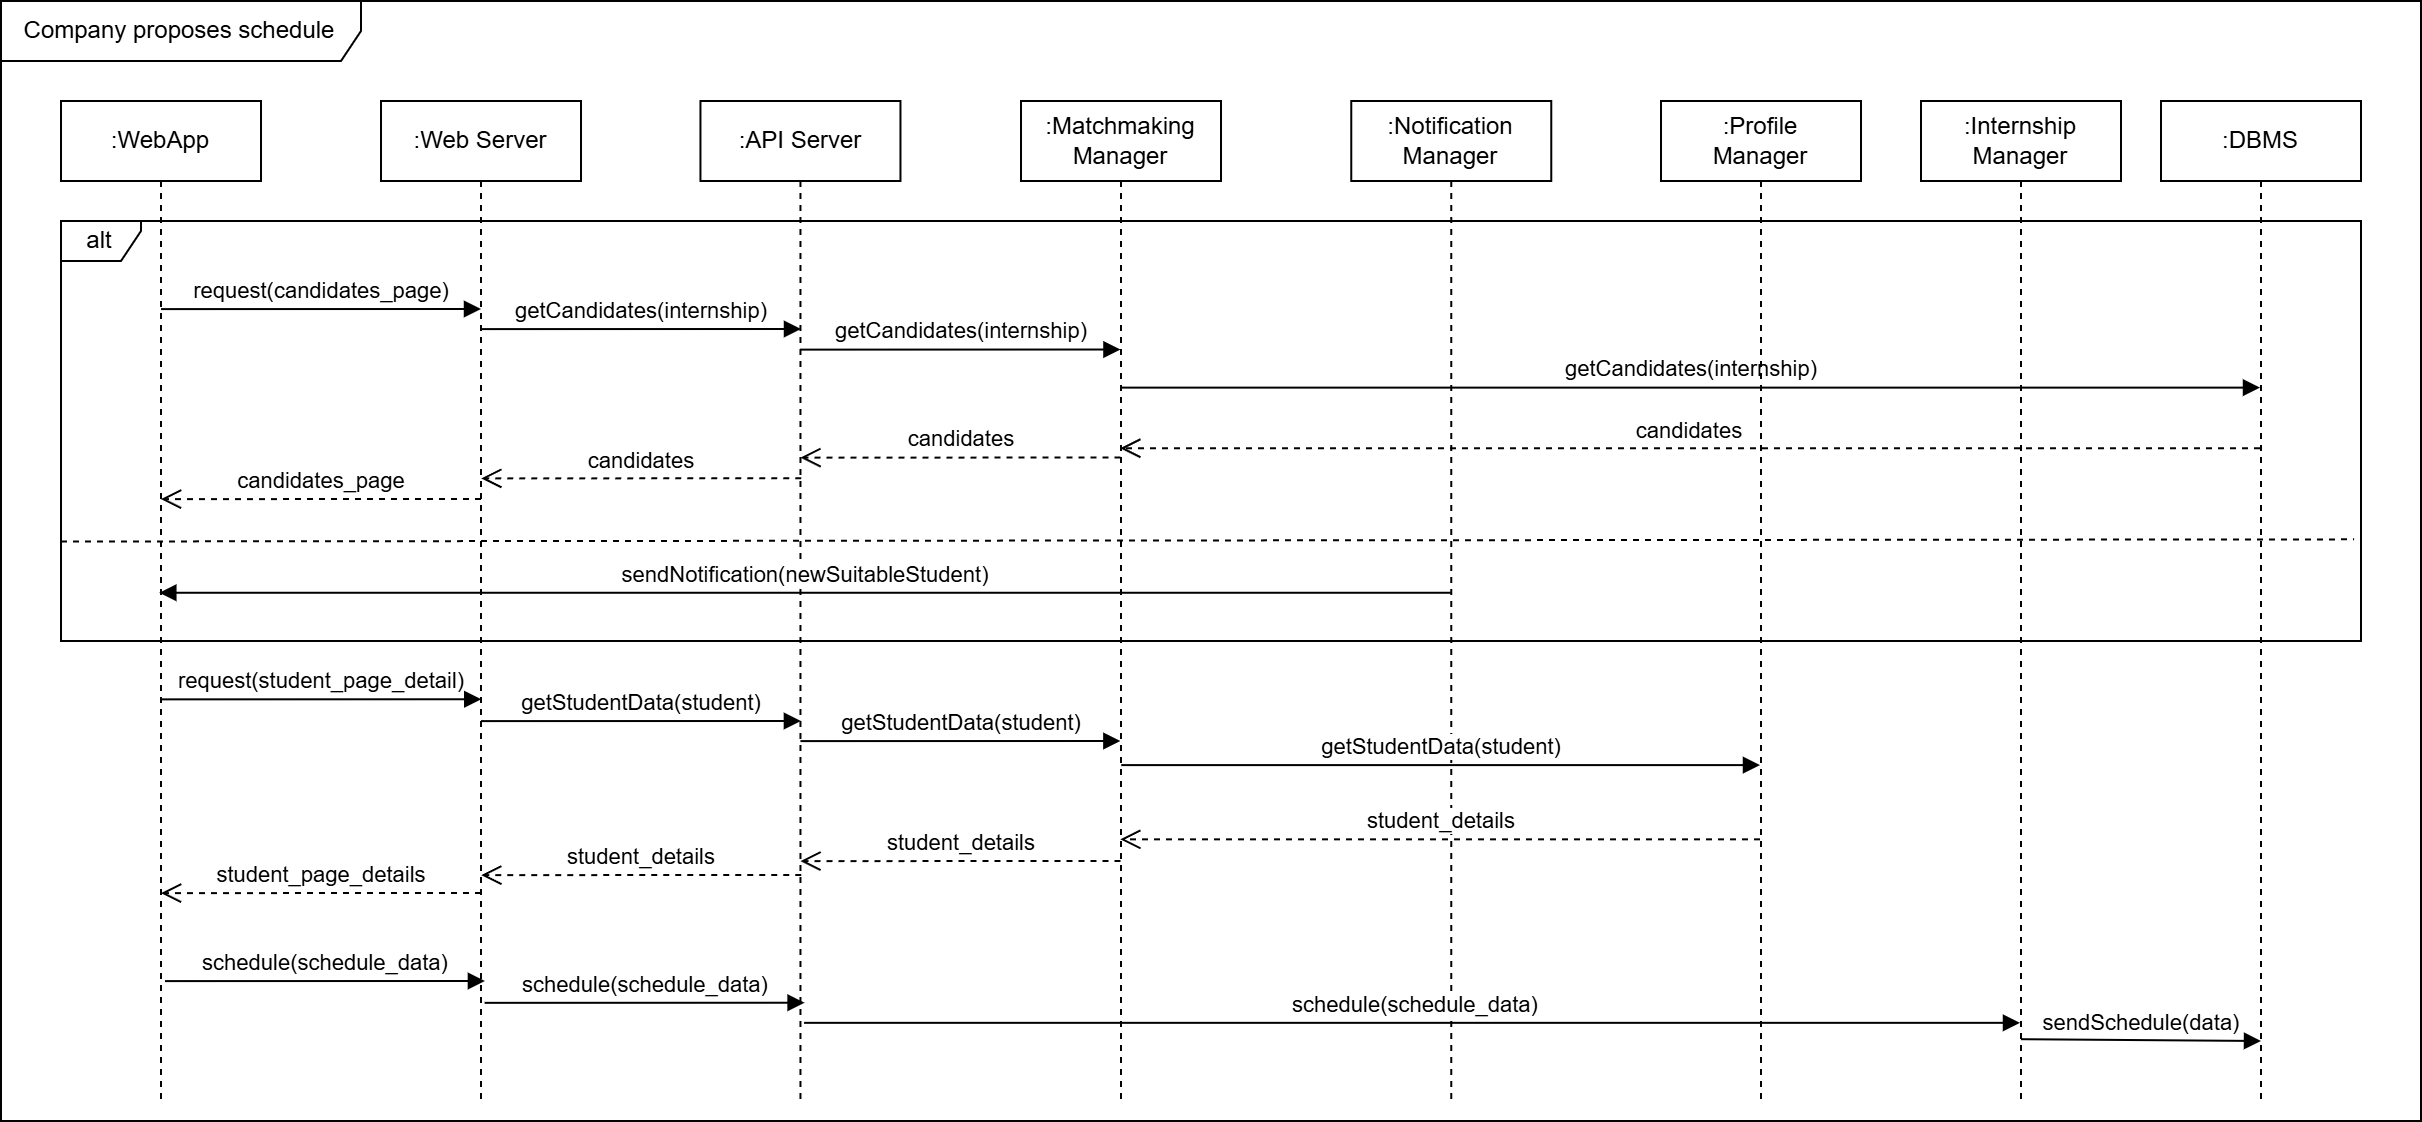
\includegraphics[width=1\linewidth]{Images/Sequence diagrams/UC13.png}
        \caption{Company schedule interview}
        \label{fig:enter-label}
    \end{figure}
\end{center}

\textbf{UC\cuc\  - Student or Company submits a complaint about an ongoing internship} \\
The figure shows the process of submitting a new complaint on an internship by a student or a company. The student or company submits it through the platform. The complaint is sent via the Web Server and API Server to the Complaint Manager, which logs the issue in the database. After the complaint is recorded, the Complaint Manager sends a notification through the Notification Manager to the student’s university to alert them about the new complaint. The system then confirms the submission with a success message or informs the user of any errors encountered during the process.
\begin{center}
    \begin{figure}[H]
        \centering
        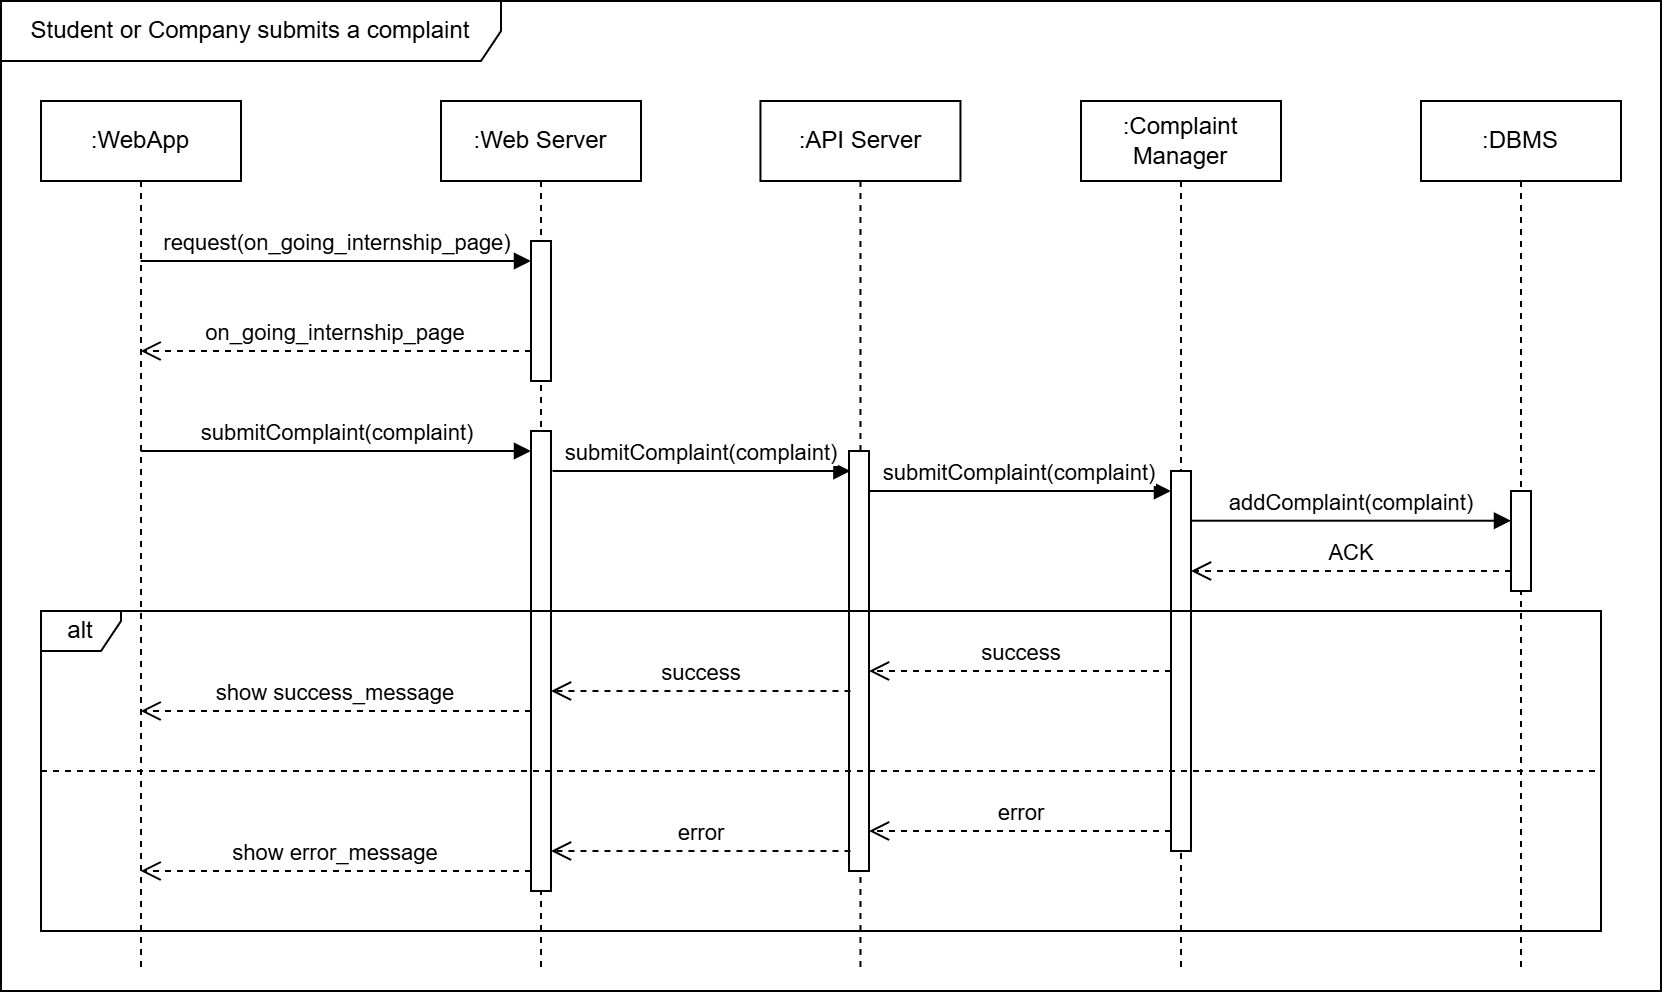
\includegraphics[width=1\linewidth]{Images/Sequence diagrams/UC14.png}
        \caption{Company new offer posting}
        \label{fig:enter-label}
    \end{figure}
\end{center}

\textbf{UC\cuc\  - Student or Company submits a feedback about a terminated internship} \\
The figure shows the process of submitting a feedback on a terminated internship by a student or a company. The student or company submits it through the platform. The feedback is processed via the Web Server and API Server and stored in the database by the Feedback Manager. After successfully recording the feedback, the system confirms the submission with a success message or informs the user of any errors. Additionally, the Feedback will be used for future analysis and reference.
\begin{center}
    \begin{figure}[H]
        \centering
        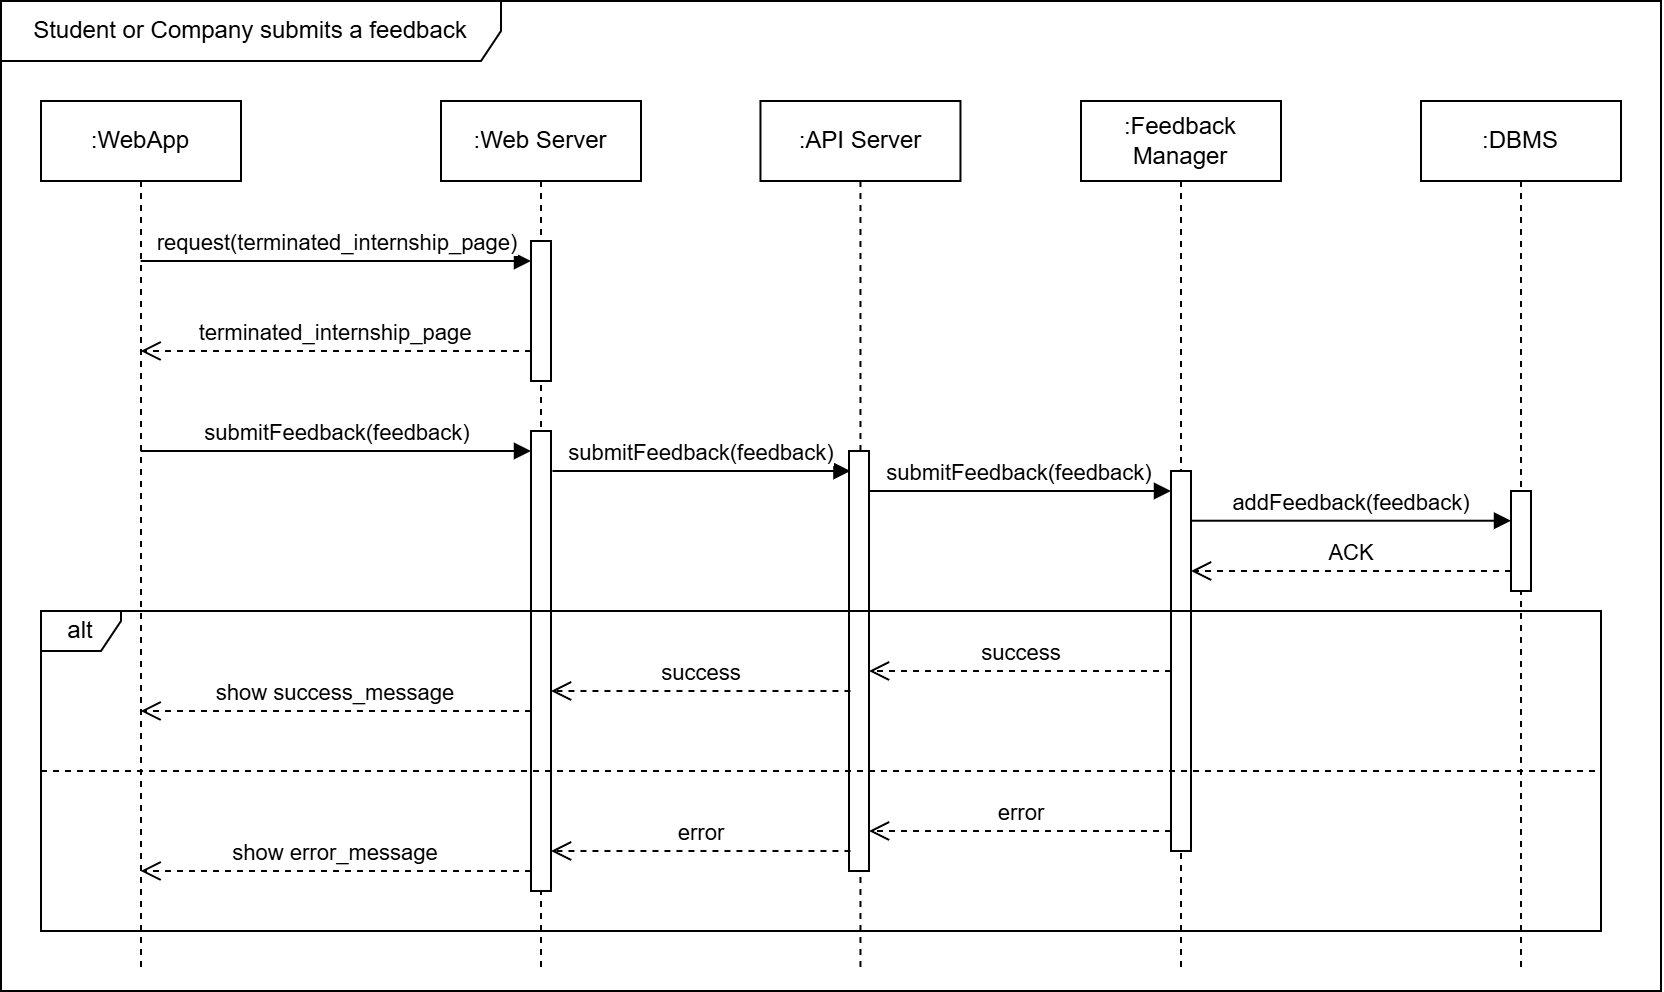
\includegraphics[width=1\linewidth]{Images/Sequence diagrams/UC15.png}
        \caption{Company new offer posting}
        \label{fig:enter-label}
    \end{figure}
\end{center}

\textbf{UC\cuc\  - University decides to interrupt an internship due to relevant complaints} \\
The figure shows the process of interrupting an internship. The university reviews relevant complaints about an ongoing internship and decides to interrupt it. The decision is submitted through the platform and processed via the Web Server and API Server. The Internship Manager updates the database to mark the internship as interrupted and notifies both the company and the student about the decision. A confirmation message is displayed to the university upon successful completion.
\begin{center}
    \begin{figure}[H]
        \centering
        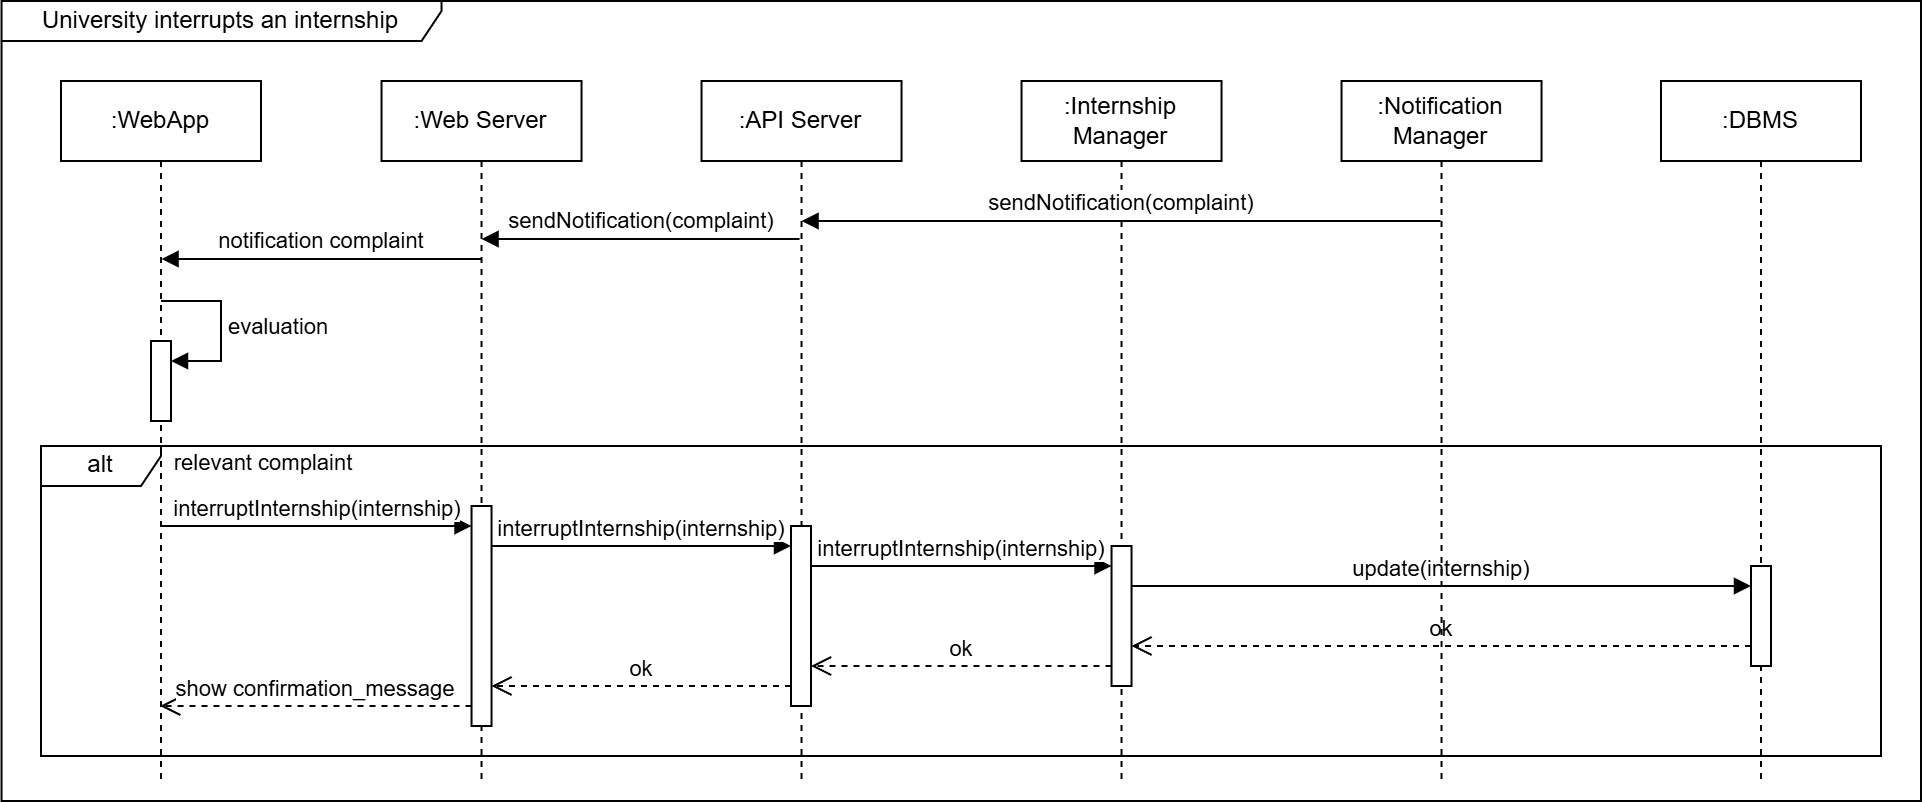
\includegraphics[width=1\linewidth]{Images/Sequence diagrams/UC16.png}
        \caption{Company new offer posting}
        \label{fig:enter-label}
    \end{figure}
\end{center}

% Add runtime view details here.

\section{Component Interfaces}
\label{sec:component_interfaces}
\textbf{Login manager}
\begin{itemize}
    \item \textit{login(String username, String password): boolean}
\end{itemize}
\textbf{Registration manager}
\begin{itemize}
\item \textit{register(String name, String surname, String email) : Boolean}
    \item \textit{upgradeToStudentAccount(User user, String name, String surname, String academicEmail, String phoneNumber, String postalCode, File CV, List<String> goals): boolean}
    \item u\textit{pgradeToCompanyAccount(User user, String fullName, String phoneNumber, String officeAddress): boolean}
\end{itemize}
\textbf{Profile manager}
\begin{itemize}
    \item \textit{getStudentData(Student student): Student}
    \item \textit{updateStudentData(Student student, String name, String surname, String academicEmail, String phoneNumber, String postalCode, List<String> goals): boolean}
    \item \textit{updateStudentCV(Student student, File CV): boolean}
    \item \textit{getCompanyData(Company company): Company}
    \item \textit{updateCompanyData(Company company, String fullName, String phoneNumber, String officeAddress): boolean}
\end{itemize}
\textbf{Internship manager}
\begin{itemize}
    \item \textit{addInternshipOffer(Company company, String projectDescription, String role, String address, Float salary, Int numberOfStudents, List<String> skills, String weeklySchedule, List<String> benefits): boolean}
    \item \textit{updateInternshipOffer(Internship internship, String projectDescription, String role, String address, Float salary, Int numberOfStudents, List<String> skills, String weeklySchedule, List<String> benefits): boolean}
    \item \textit{deleteInternshipOffer(Internship internship): boolean}
    \item \textit{acceptApplication(Application application): boolean}
    \item \textit{sendSchedule(Internship internship, Student student, String schedule): boolean}
    \item \textit{rejectApplication(Application application): boolean}
    \item \textit{confirmInternship(Internship internship, Student student): boolean}
    \item \textit{rejectInternship(Internship internship, Student student): boolean}
\end{itemize}
\textbf{Matchmaking manager}
\begin{itemize}
    \item \textit{generateRecommendationsForStudent(Student student): List<Internship>}
    \item \textit{generateRecommendationsForStudent(Internship internship): List<Student>}
    \item \textit{findBestMatch(Student student): Internship}
    \item \textit{findBestMatch(Internship internship): Student}
    \item \textit{getCandidates(Internship internship): List<Student>}
\end{itemize}
\textbf{Complaint manager}
\begin{itemize}
    \item \textit{submitComplaint(Internship internship, Student student, String complaintText): boolean}
    \item \textit{submitComplaint(Internship internship, Company company, String complaintText): boolean}
    \item \textit{getComplaintStatus(Complaint complaint): ComplaintStatus}
    \item \textit{getCompliantsByInternship(Internship internship): List<Complaint>}
    \item \textit{interruptInternship(Internship internship, String reason): boolean}
\end{itemize}
\textbf{Feedback manager}
\begin{itemize}
    \item \textit{submitFeedback(Internship internship, Student student, String feedbackText): boolean}
    \item \textit{submitFeedback(Internship internship, Company company, String feedbackText): boolean}
    \item \textit{getFeedbackByInternship(Internship internship): List<Feedback>}
    \item \textit{analyzeFeedback(Feedback feedback): boolean}
\end{itemize}
\textbf{Notification manager}
\begin{itemize}
    \item \textit{sendNotification(User user, NotificationType type, String message): boolean}
    \item \textit{getNotifications(User user): List<Notification>}
\end{itemize}

% Describe the component interfaces here.

\section{Selected Architectural Styles and Patterns}
\label{sec:architectural_styles_patterns}
\subsection{3-tiered Architecture}
The architectural style chosen is 3-tiered architecture, which provides significant benefits such as modularization into three distinct layers:
\begin{itemize}
    \item Web and Mobile Client : This is the presentation tier and gives access to the user interface. The web application provides the user interface through a browser, utilizing technologies like HTML, CSS, and JavaScript for dynamic and interactive content. The mobile application delivers a native or hybrid experience, optimized for smaller screens and supporting additional functionalities like push notifications.
    \item The S\&C API server : This is the middle tier, responsible for implementing the business logic of the system. It handles tasks such as user authentication, internship matching, and processing of user actions. The application server communicates with the database server and ensures the seamless operation of system workflows.
    \item The database server : This is the backend of the application, powered by a Database Management System (DBMS) like MySQL. It stores and manages all system data, including user profiles, internship postings, applications, complaints and feedback, ensuring data integrity and quick retrieval for the application server.
\end{itemize}
% Add information about architectural styles and patterns here.

\section{Other Design Decisions}
\label{sec:other_design_decisions}
This section is focused on explaining the design decisions  that have been implemented in order to make the system work correctly.
\subsection{Availability}
Load balancing is implemented to create a system with a high availability and capable of handling a large amount of concurrent requests efficiently. In addition to this, it is crucial to incorporate replication mechanism in order to eliminate single points of failure and enhance system reliability.
\subsection{Data Storage}
Data storage is managed through the use of a database to store the personal information of users, students, universities and companies. Additionally, auxiliary data structures are used in order to make query performance better. 


    \chapter{User Interface Design}
    \label{ch:user_interface_design}%
    In this section, an overview of the user interface of the S\&C system is presented.
The focus is primarily on the user experience, with secondary attention given to the user interface. Although the interface has been carefully designed, it remains subject to refinement based on feedback from usability testing and focus groups.
The mock-ups shown below include both the desktop browser version and the mobile application version, allowing us to showcase the interface for both Student and Company users. The desktop version provides full access to all functionalities, while the mobile version, designed to be fully responsive, ensures a seamless experience across devices regardless of screen size or user type.

\section{General overview}
The image below illustrates the structure of the pages accessible within the S\&C application.
All pages are accessible only after logging into the main login page, which serves as a gateway separating Student, Company and University dashboards.

\begin{figure}[H]
    \centering
        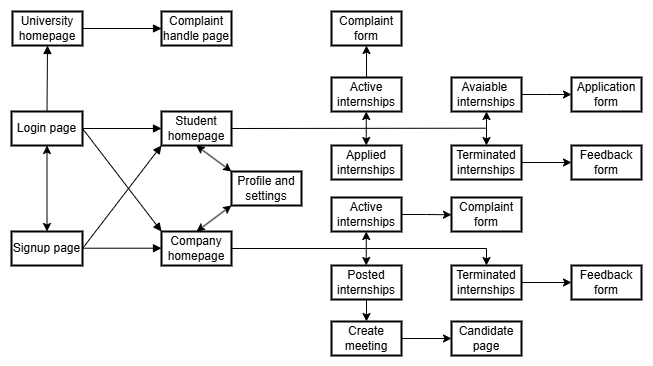
\includegraphics[width=1\linewidth]{Images/Mock-up/User interface overview.png}
    \caption{S\&C overview}
    \label{fig:homepage-design}
\end{figure}

As previously mentioned, the login section is the entry point for users, allowing them, upon successful authentication, to access their respective dashboards and interact with the system’s features. In S\&C, there are three primary types of dashboards corresponding to the three main user roles involved in the system’s processes: Students, Companies and Universities.

While the dashboards slightly in their aesthetic choices (such as color schemes), they maintain a consistent structure and layout. This design decision was made to optimize development by relying on reusable components, ensuring a scalable and maintainable interface that can be efficiently updated over time.

From the Company dashboard, the following pages can be accessed:
\begin{itemize}
    \item Company Profile Management – For updating and managing company information
    \item Post a New Internship and Manage Existing Internships – To create internship opportunities and oversee the ones already posted.
    \item View Applications and Contact Students – To review applications submitted by students and/or initiate communication with potential candidates.
    \item Submit a Complaint for Active Internships – A page dedicated to reporting issues related to ongoing internships. 
    \item Submit Feedback for Terminated Internships – A page for providing feedback on completed internships.
\end{itemize}

From the Student dashboard, the following pages can be accessed:
\begin{itemize}
    \item Student Profile Management – To update personal details, academic information, and preferences.
    \item Internship Search and Application – To browse available internships and submit applications.
    \item Submit a Complaint for Active Internships – To report issues or challenges encountered during an ongoing internship.
    \item Submit Feedback for Terminated Internships – To provide feedback about completed internship experiences.
\end{itemize}

From the University dashboard, the following page can be accessed:
\begin{itemize}
    \item Complaint Management – To review and handle complaints submitted by students enrolled at the university regarding their ongoing internships.
\end{itemize}

Additionally, both dashboards provide users with targeted notifications relevant to their role. All the pages outlined above will be described in greater detail in the following sections. \\

\begin{figure}[H]
    \centering
    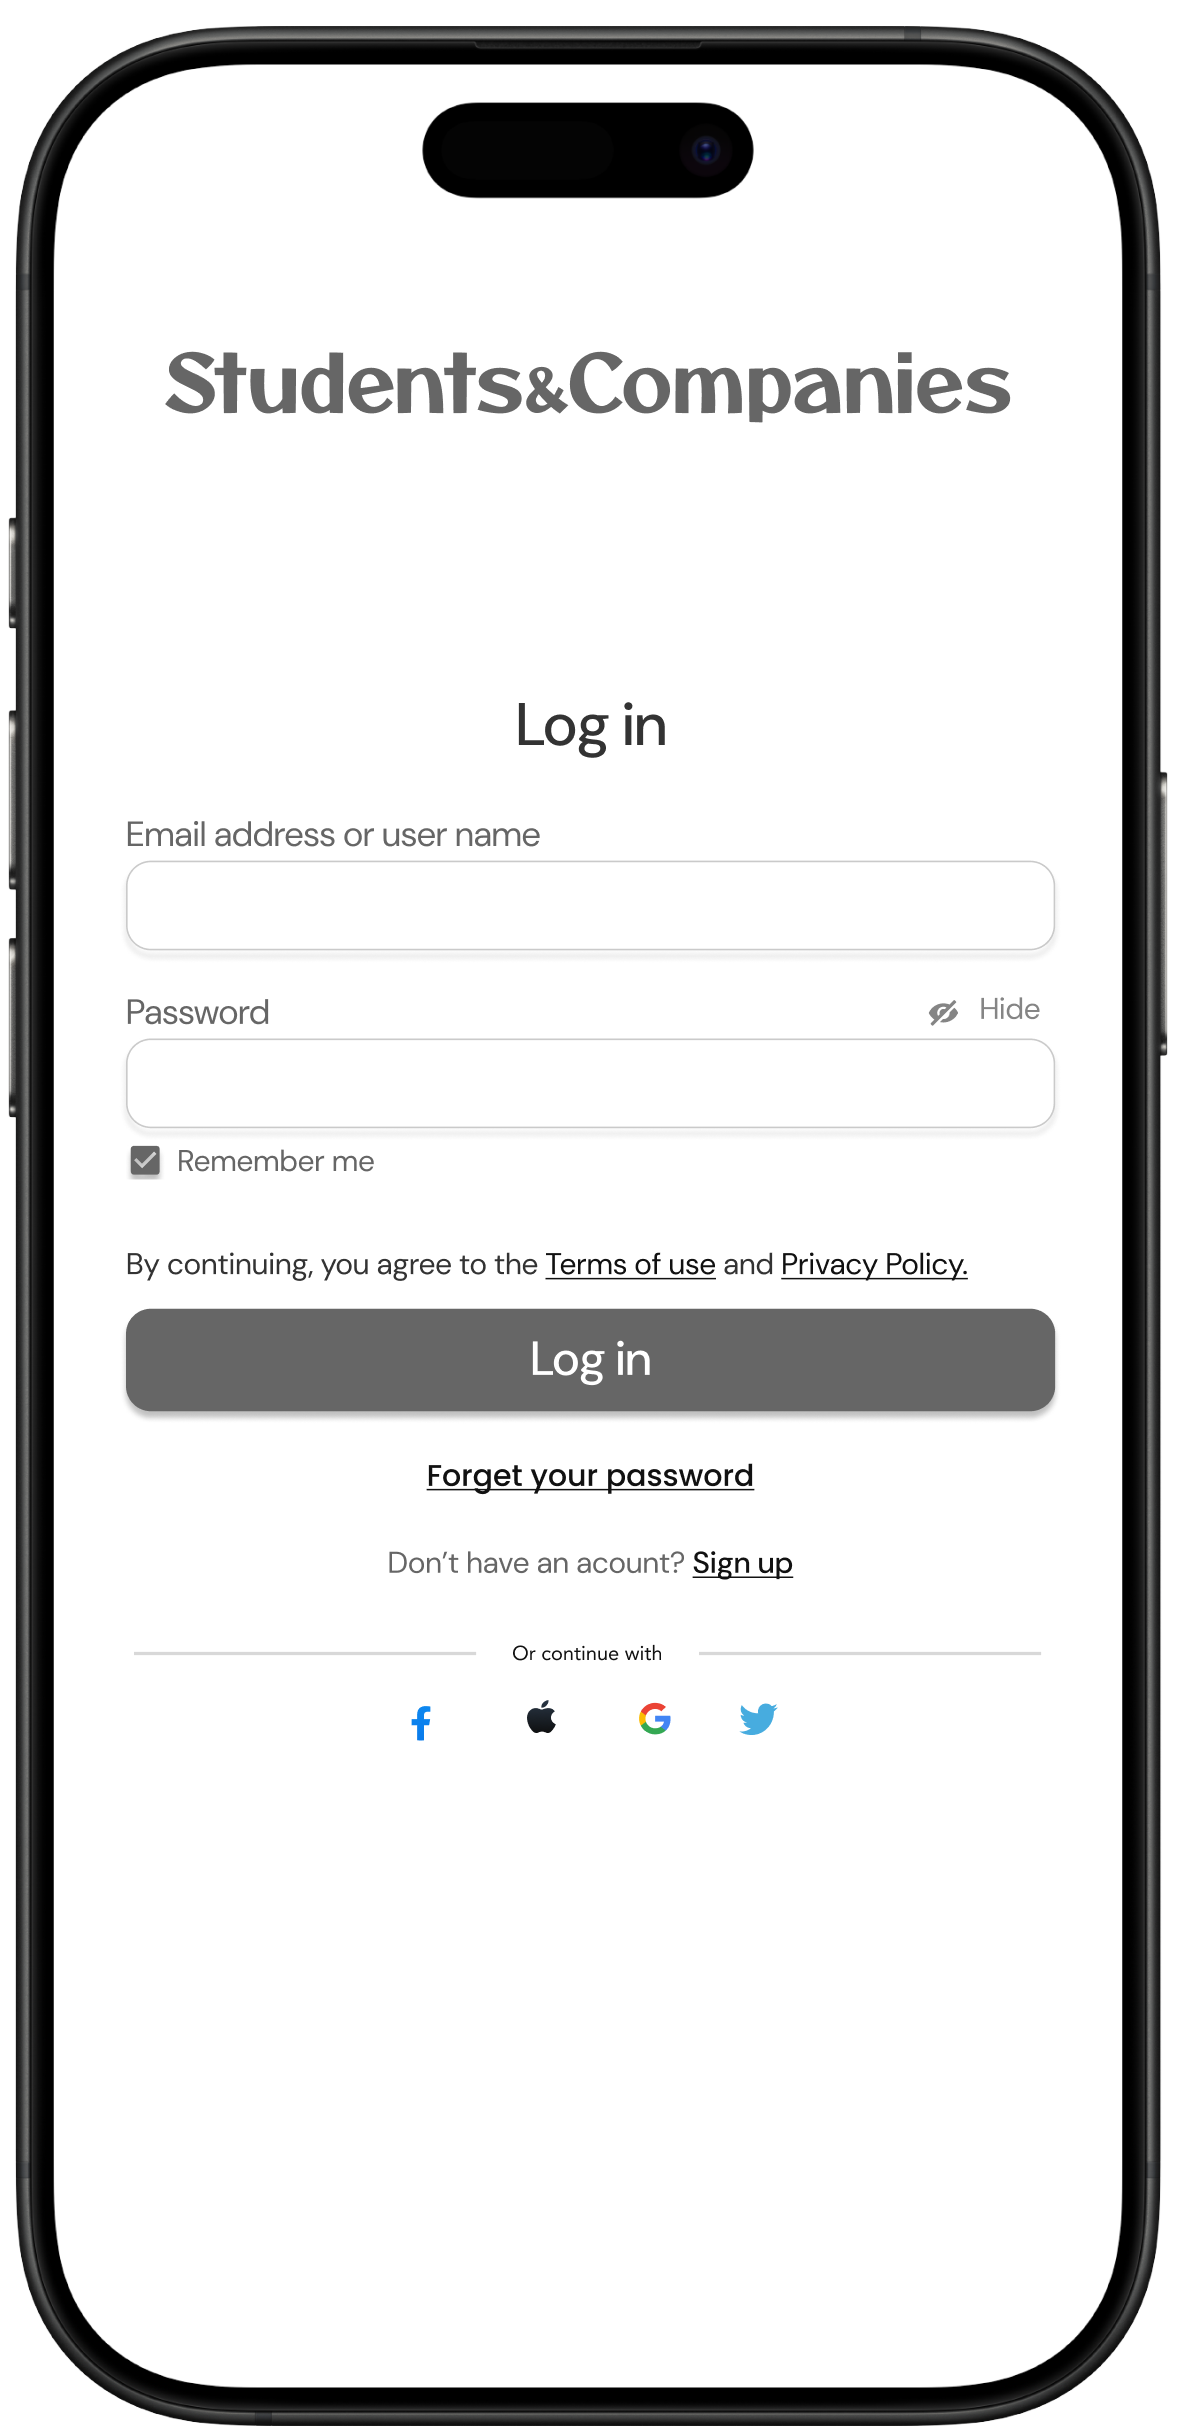
\includegraphics[width=0.2\linewidth]{Images/Mock-up/LoginInterfaceMobile.png}
    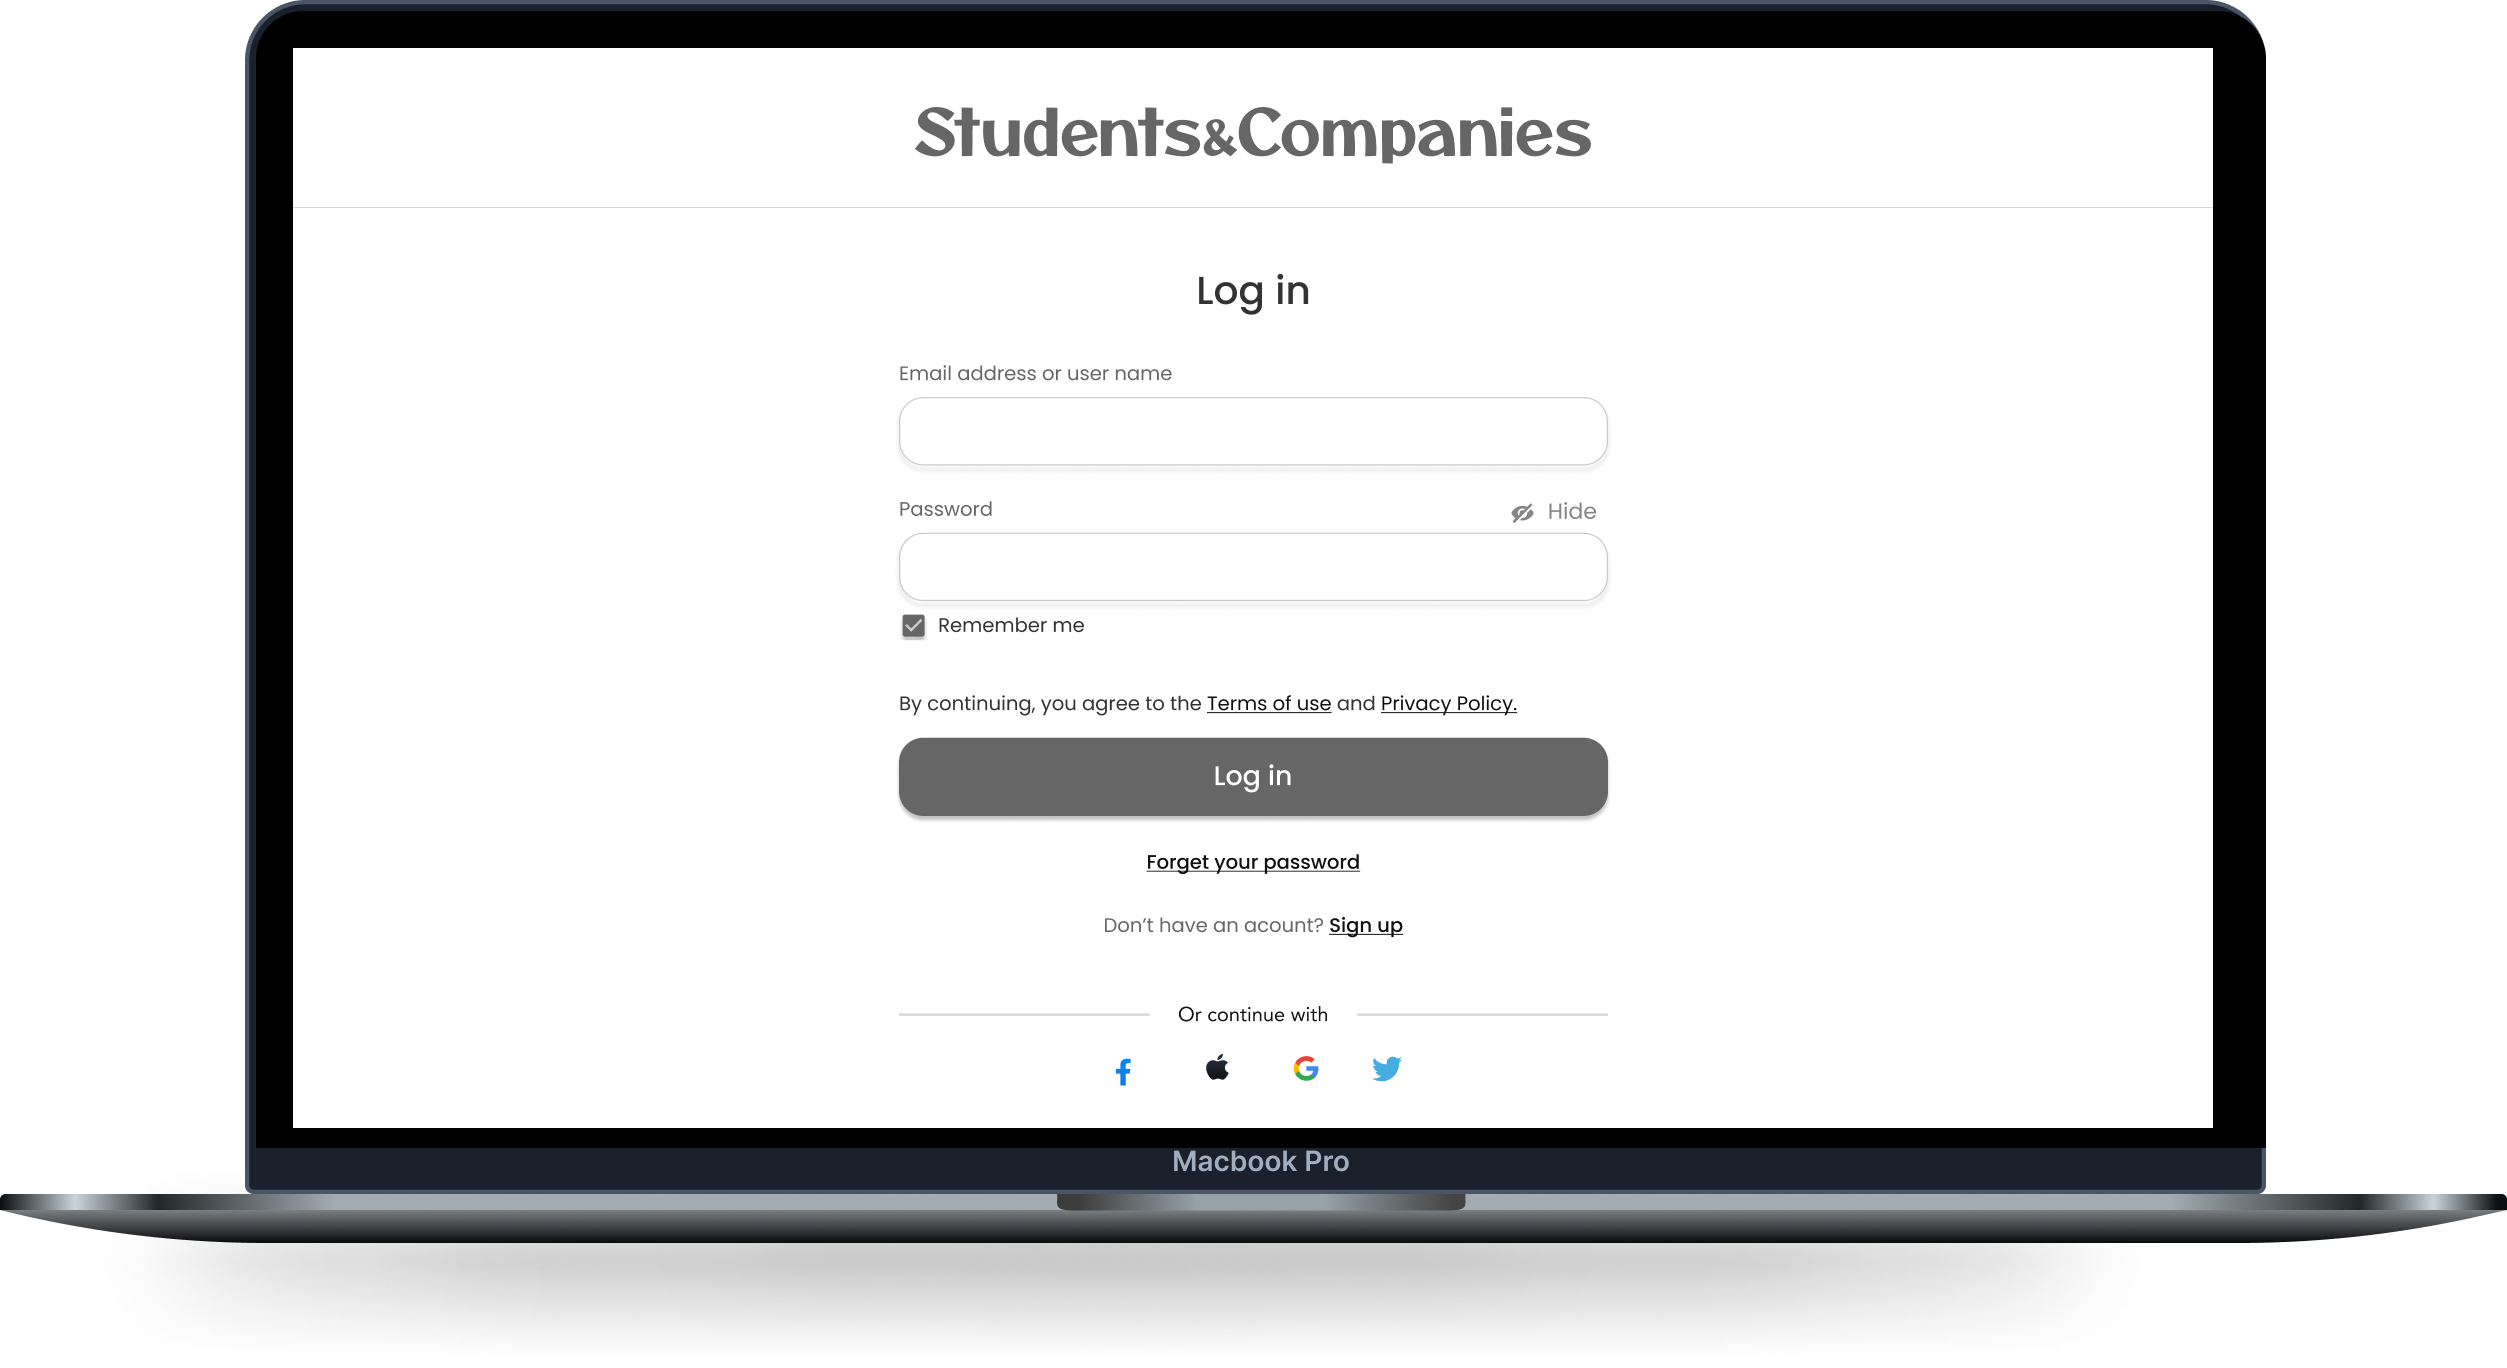
\includegraphics[width=0.75\linewidth]{Images/Mock-up/LoginPagePC.png}
    \caption{S\&C Login Page Design}
    \label{fig:homepage-design}
\end{figure}

\subsection{Registration Interface}
The registration interface is designed to allow users, whether students or companies, to create an account on the S\&C platform. The mockup showcases a simple and intuitive form where users are required to input their email address and choose a secure password, which must be confirmed by re-entering it. To proceed, users must also agree to the platform’s Terms and Conditions and Privacy Policy by selecting the appropriate checkboxes.

Once the form is submitted, the system sends a confirmation email to the address provided by the user. This email contains a unique link that, when clicked, activates the user’s account. \\

\begin{figure}[H]
    \centering
    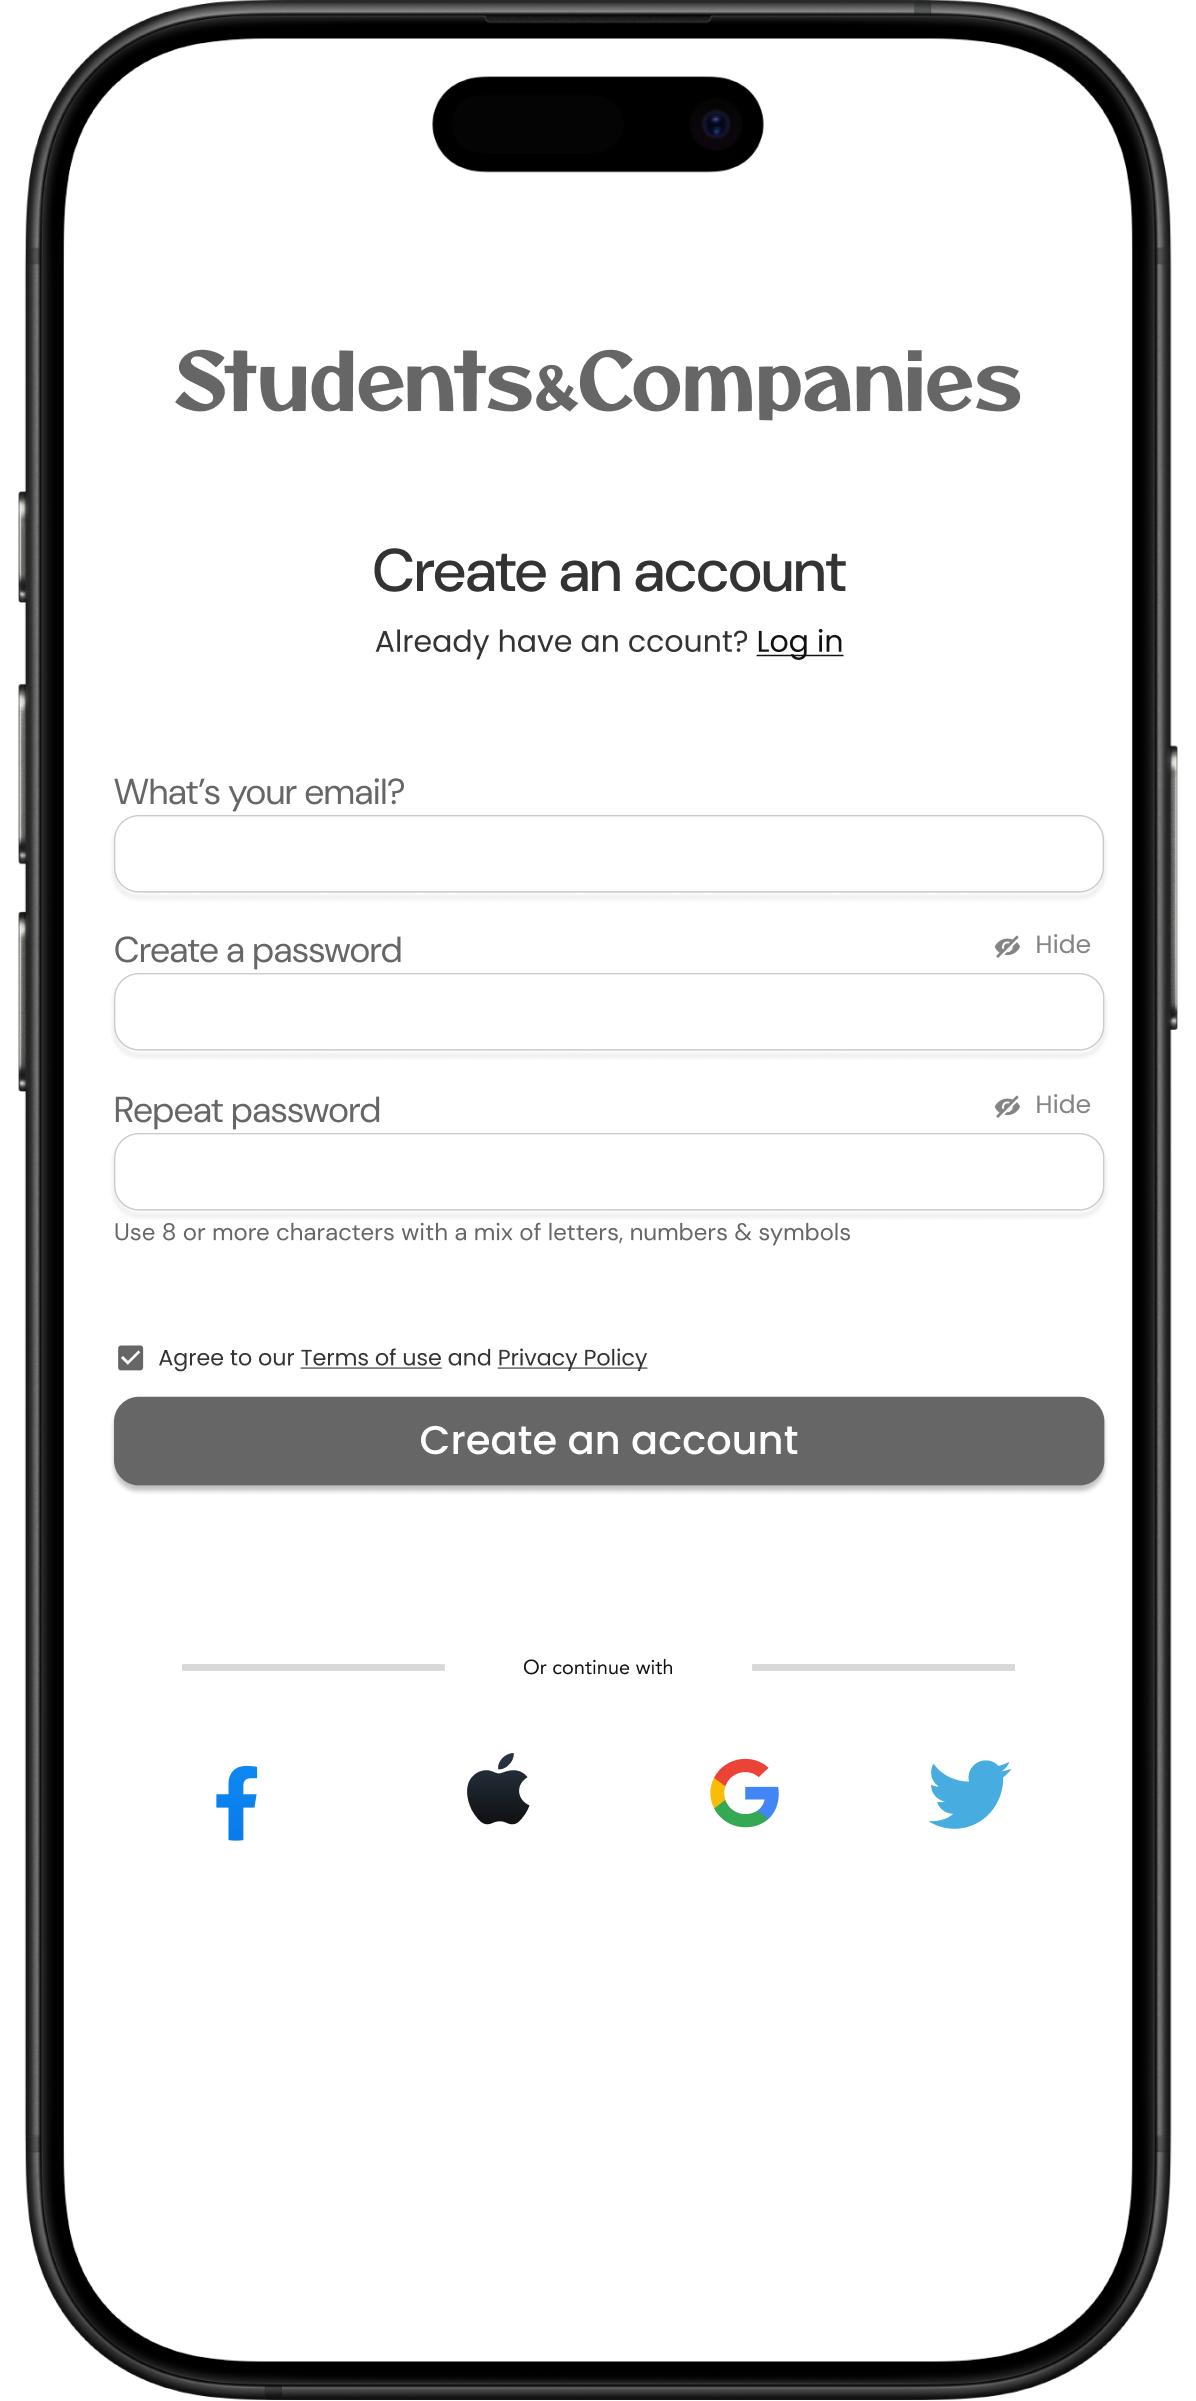
\includegraphics[width=0.2\linewidth]{Images/Mock-up/RegistrationMobile.png}
    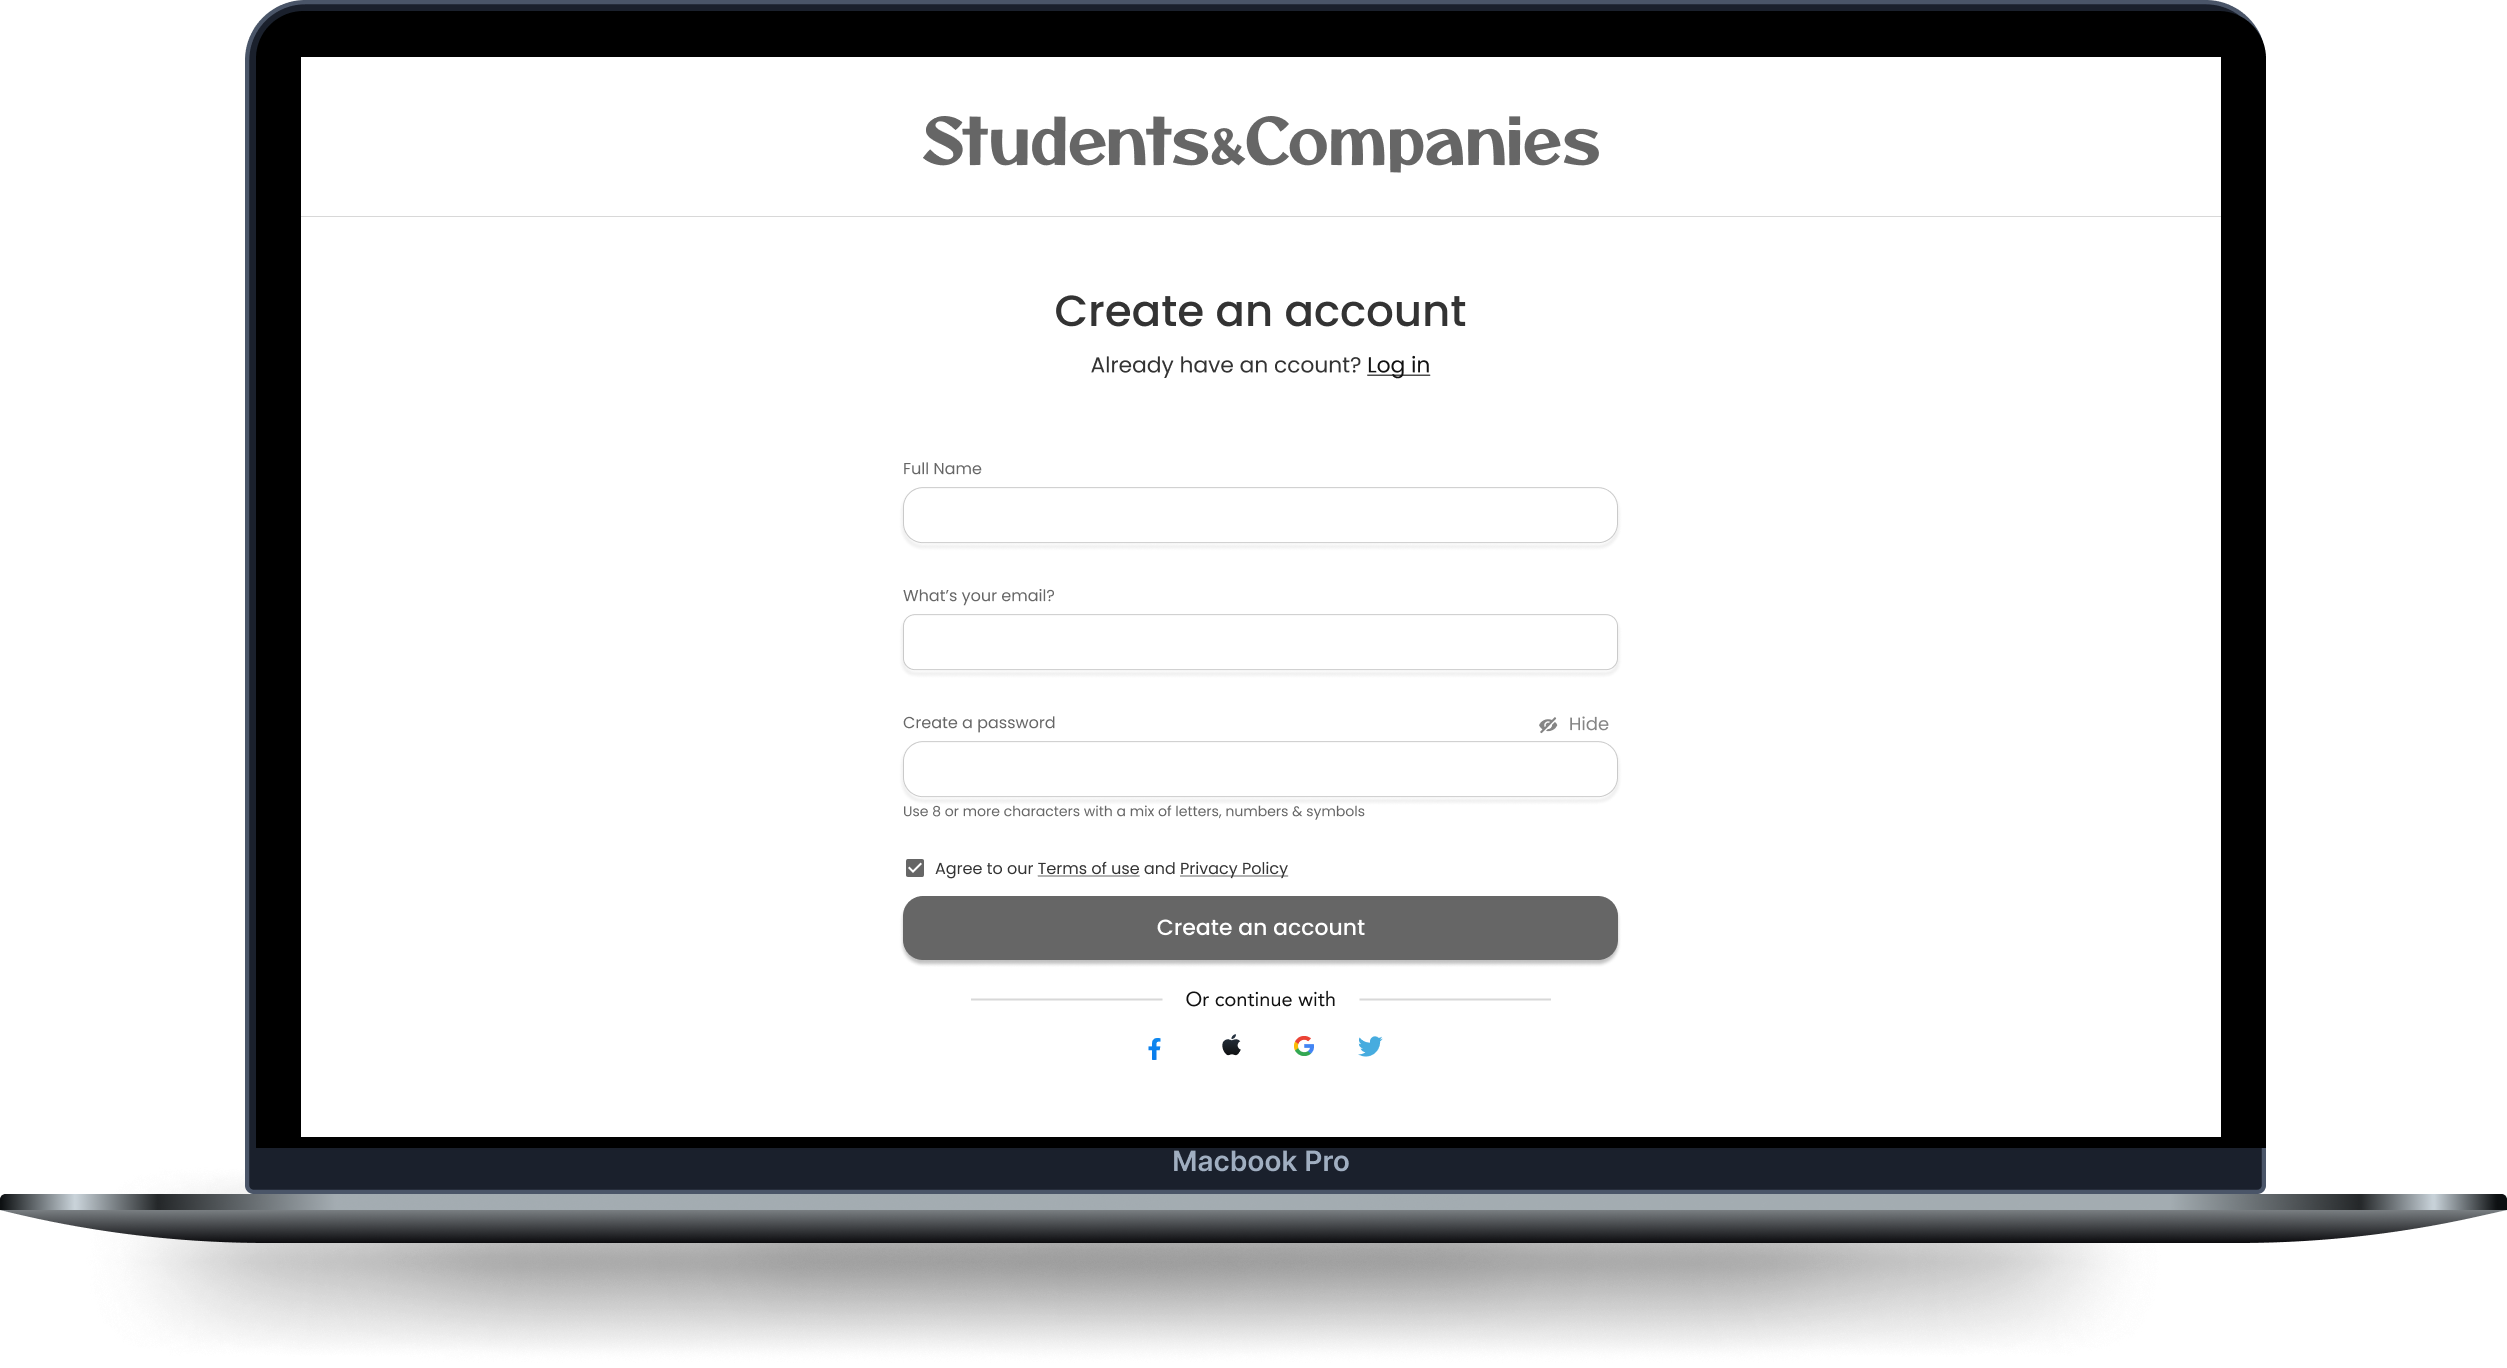
\includegraphics[width=0.75\linewidth]{Images/Mock-up/RegistrationPagePC.png}
    \caption{S\&C Registration Page Design}
    \label{fig:homepage-design}
\end{figure}

\subsection{Upgrade to Student Account Interface}

Registered users who have not yet selected a role can access this page by clicking "Upgrade account" on the generic homepage and then selecting "Upgrade to student." Here, they can complete the registration by filling out all the required fields, as personal data, goals and uploading their CV, in the form or return to the homepage without completing the action. \\

\begin{figure}[H]
    \centering
    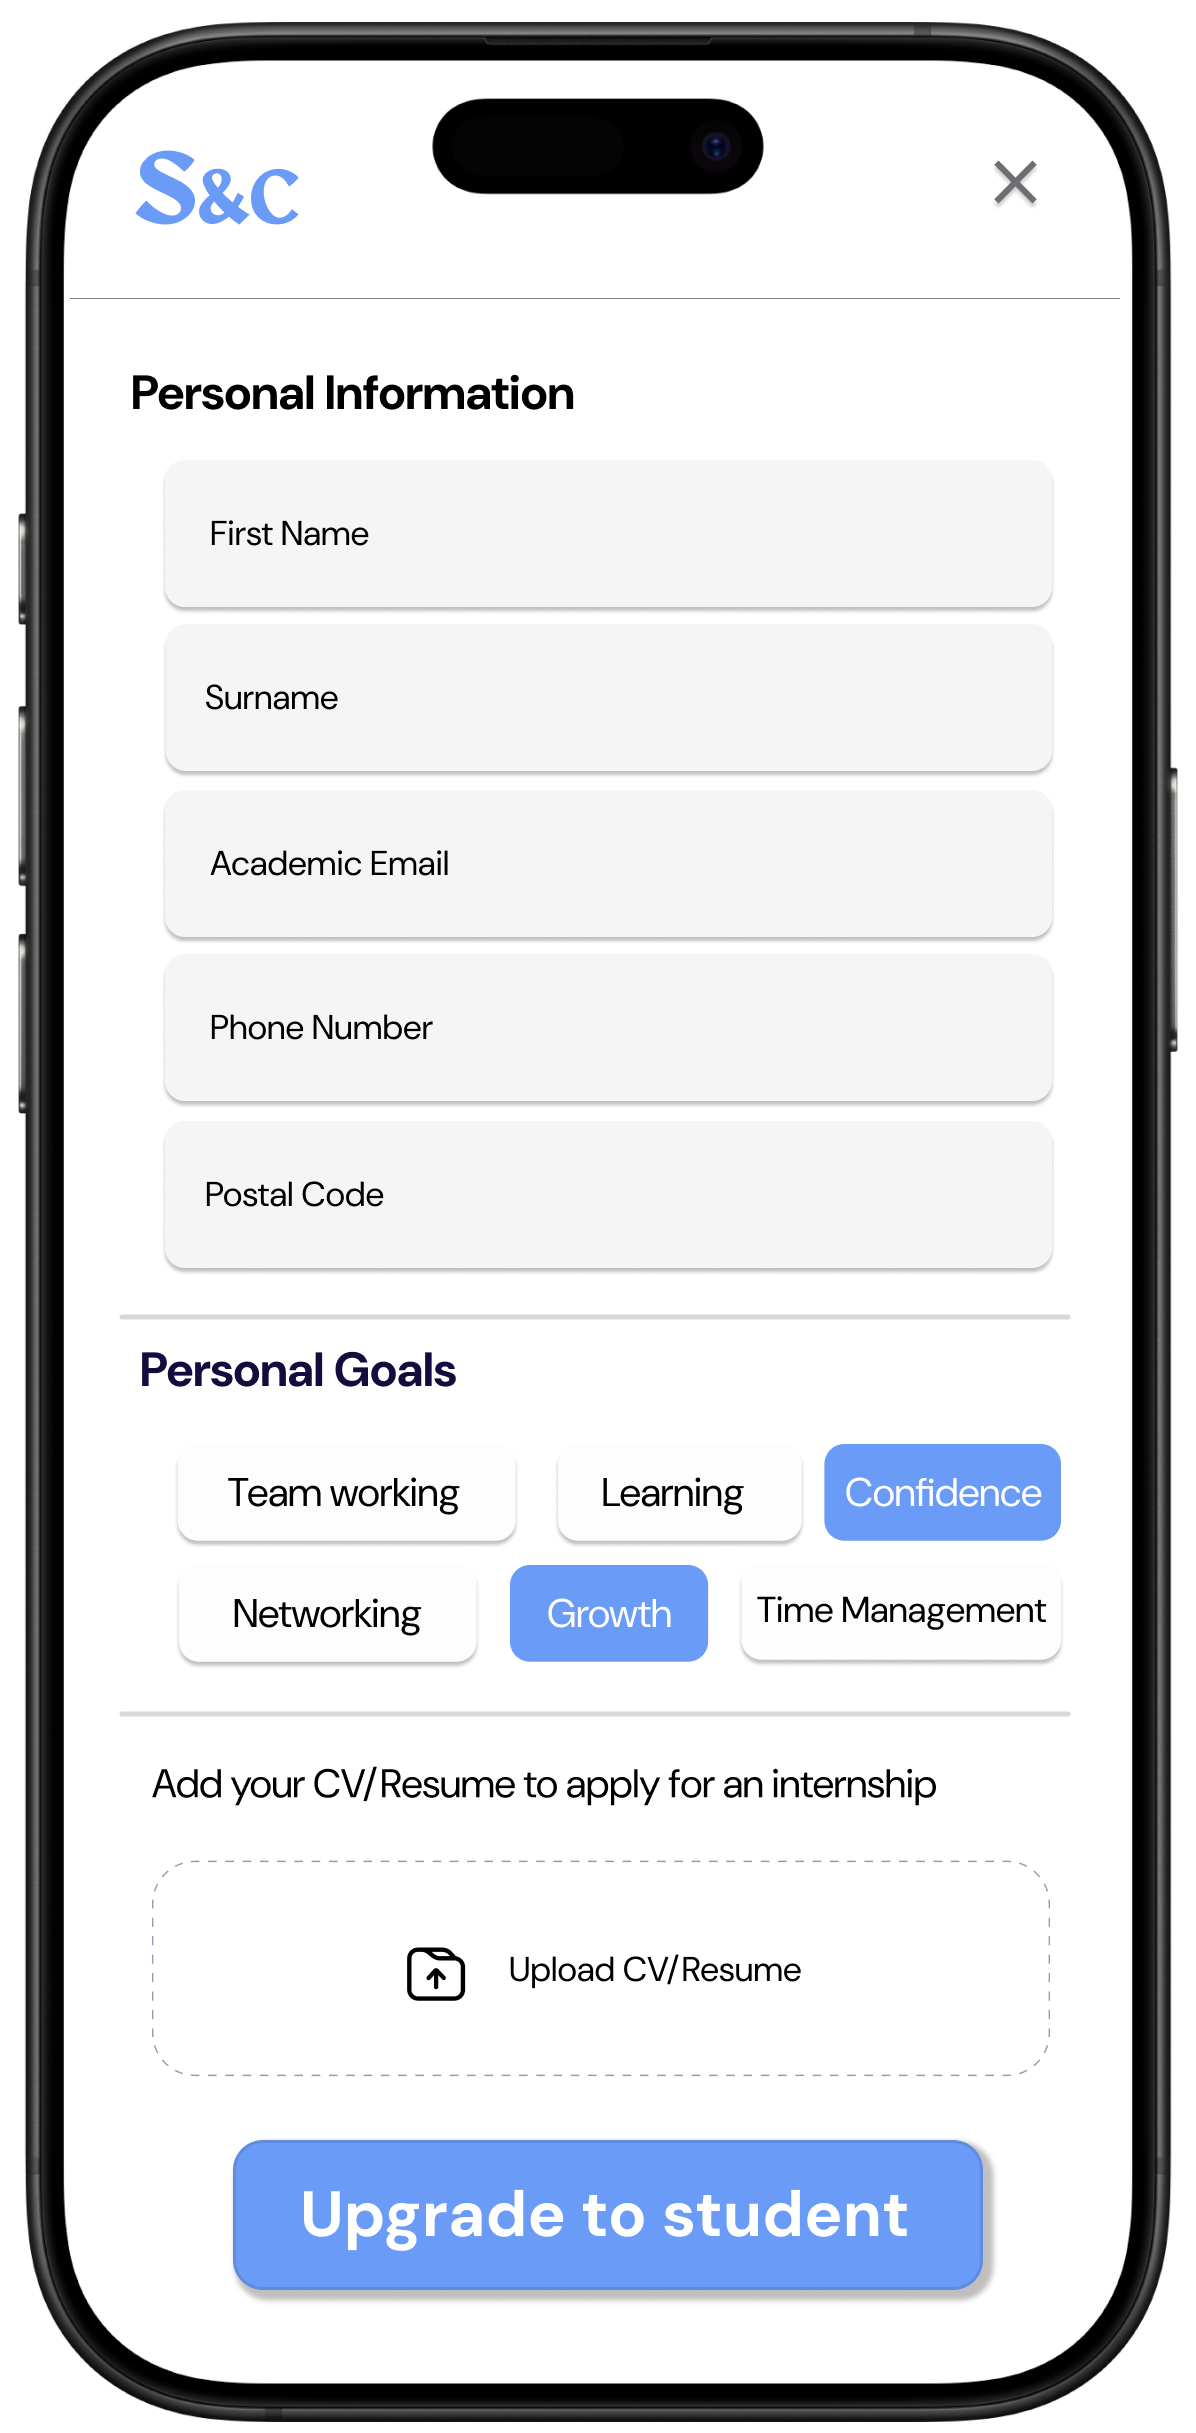
\includegraphics[width=0.2\linewidth]{Images/Mock-up/mobile upgrade to student.png}
    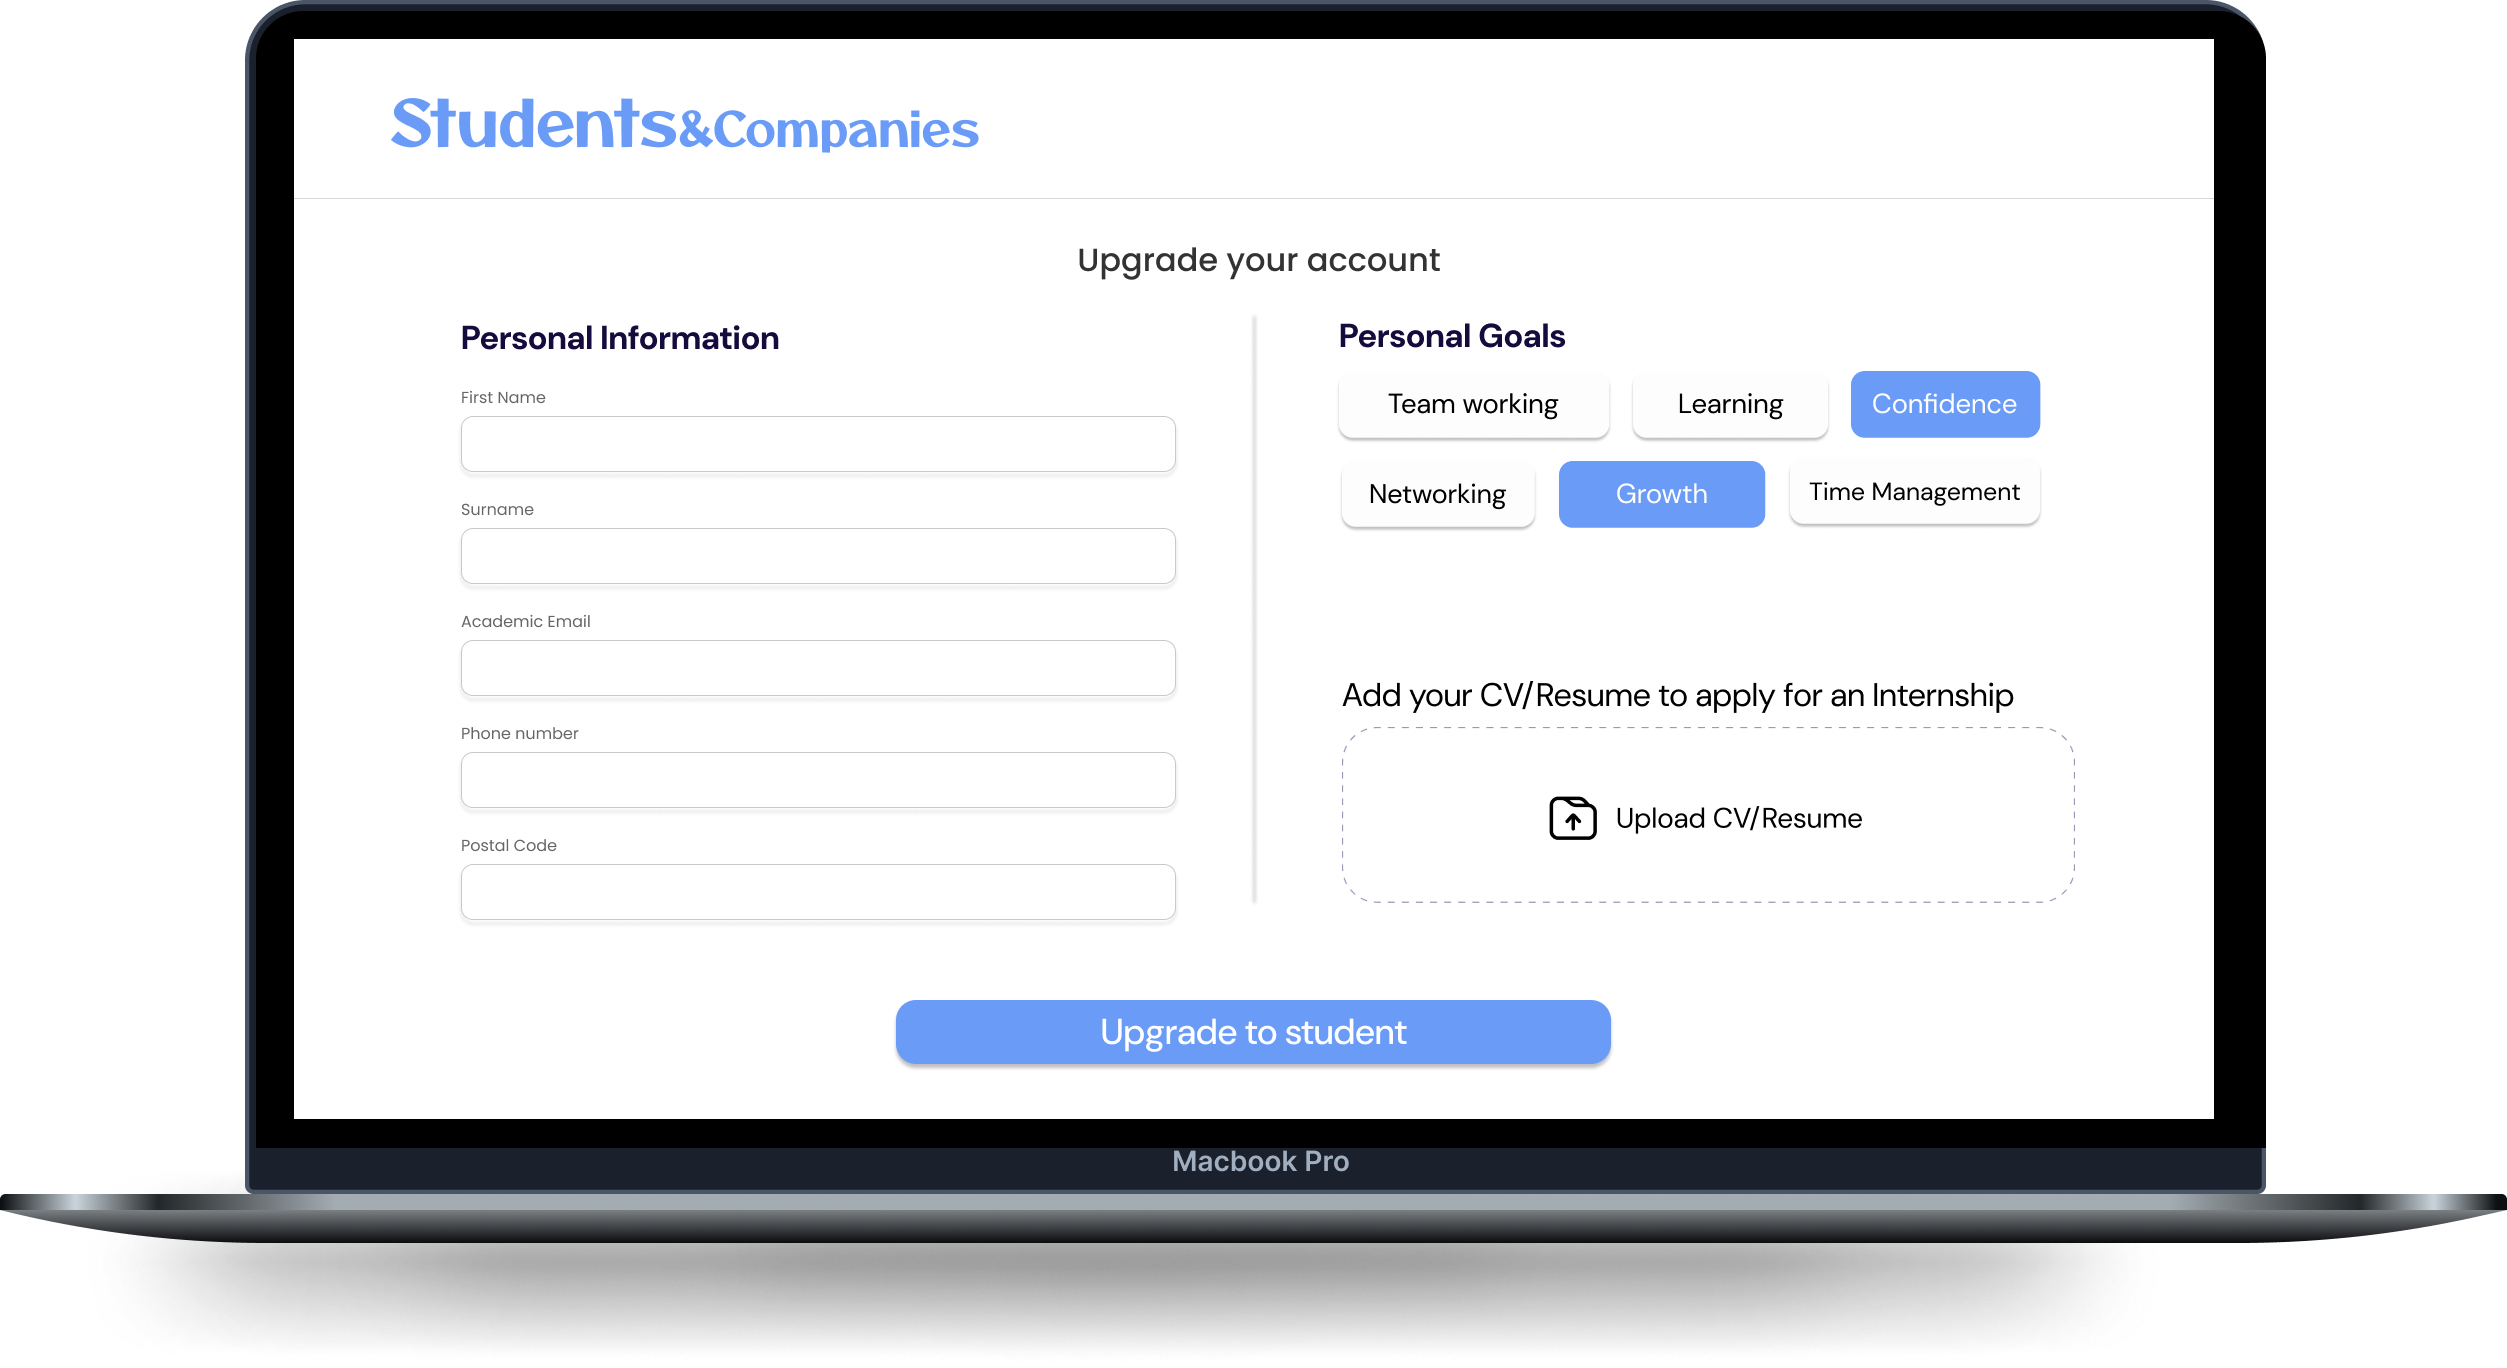
\includegraphics[width=0.75\linewidth]{Images/Mock-up/Upgrade to student.png}
    \caption{S\&C Student Account Activation Page Design}
    \label{fig:homepage-design}
\end{figure}

\subsection{Upgrade to Company Account Interface}

Registered users who have not yet selected a role can access this page by clicking "Upgrade account" on the generic homepage and then selecting "Upgrade to company." Here, they can complete the registration by filling out all the required fields about company's data in the form or return to the homepage without completing the action. \\

\begin{figure}[H]
    \centering
    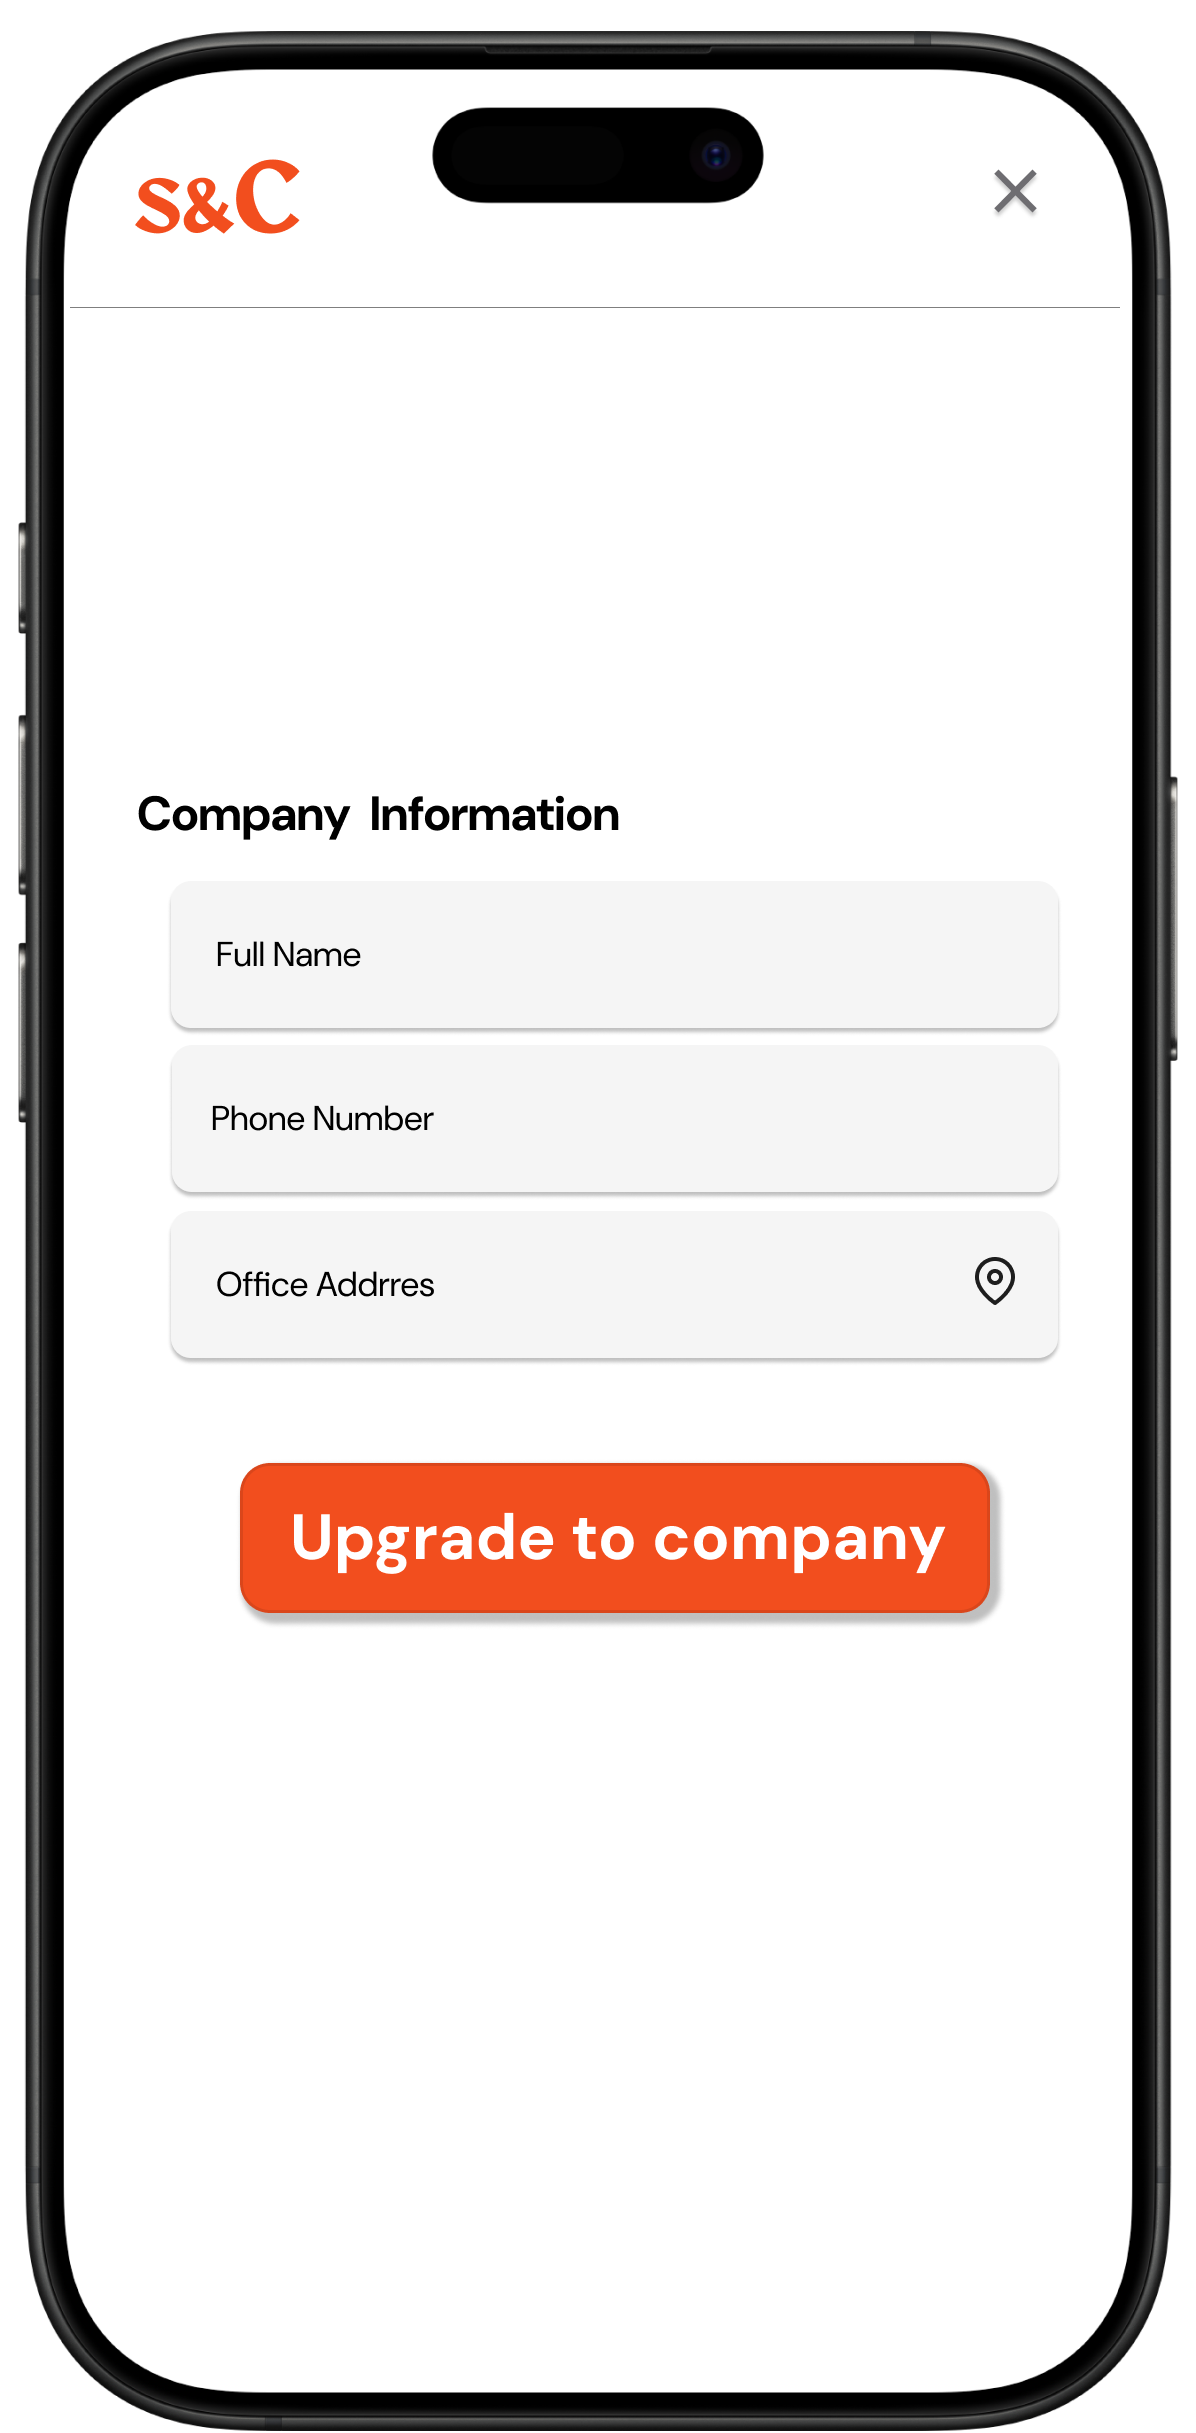
\includegraphics[width=0.2\linewidth]{Images/Mock-up/UpgradeToCompanyMobile.png}
    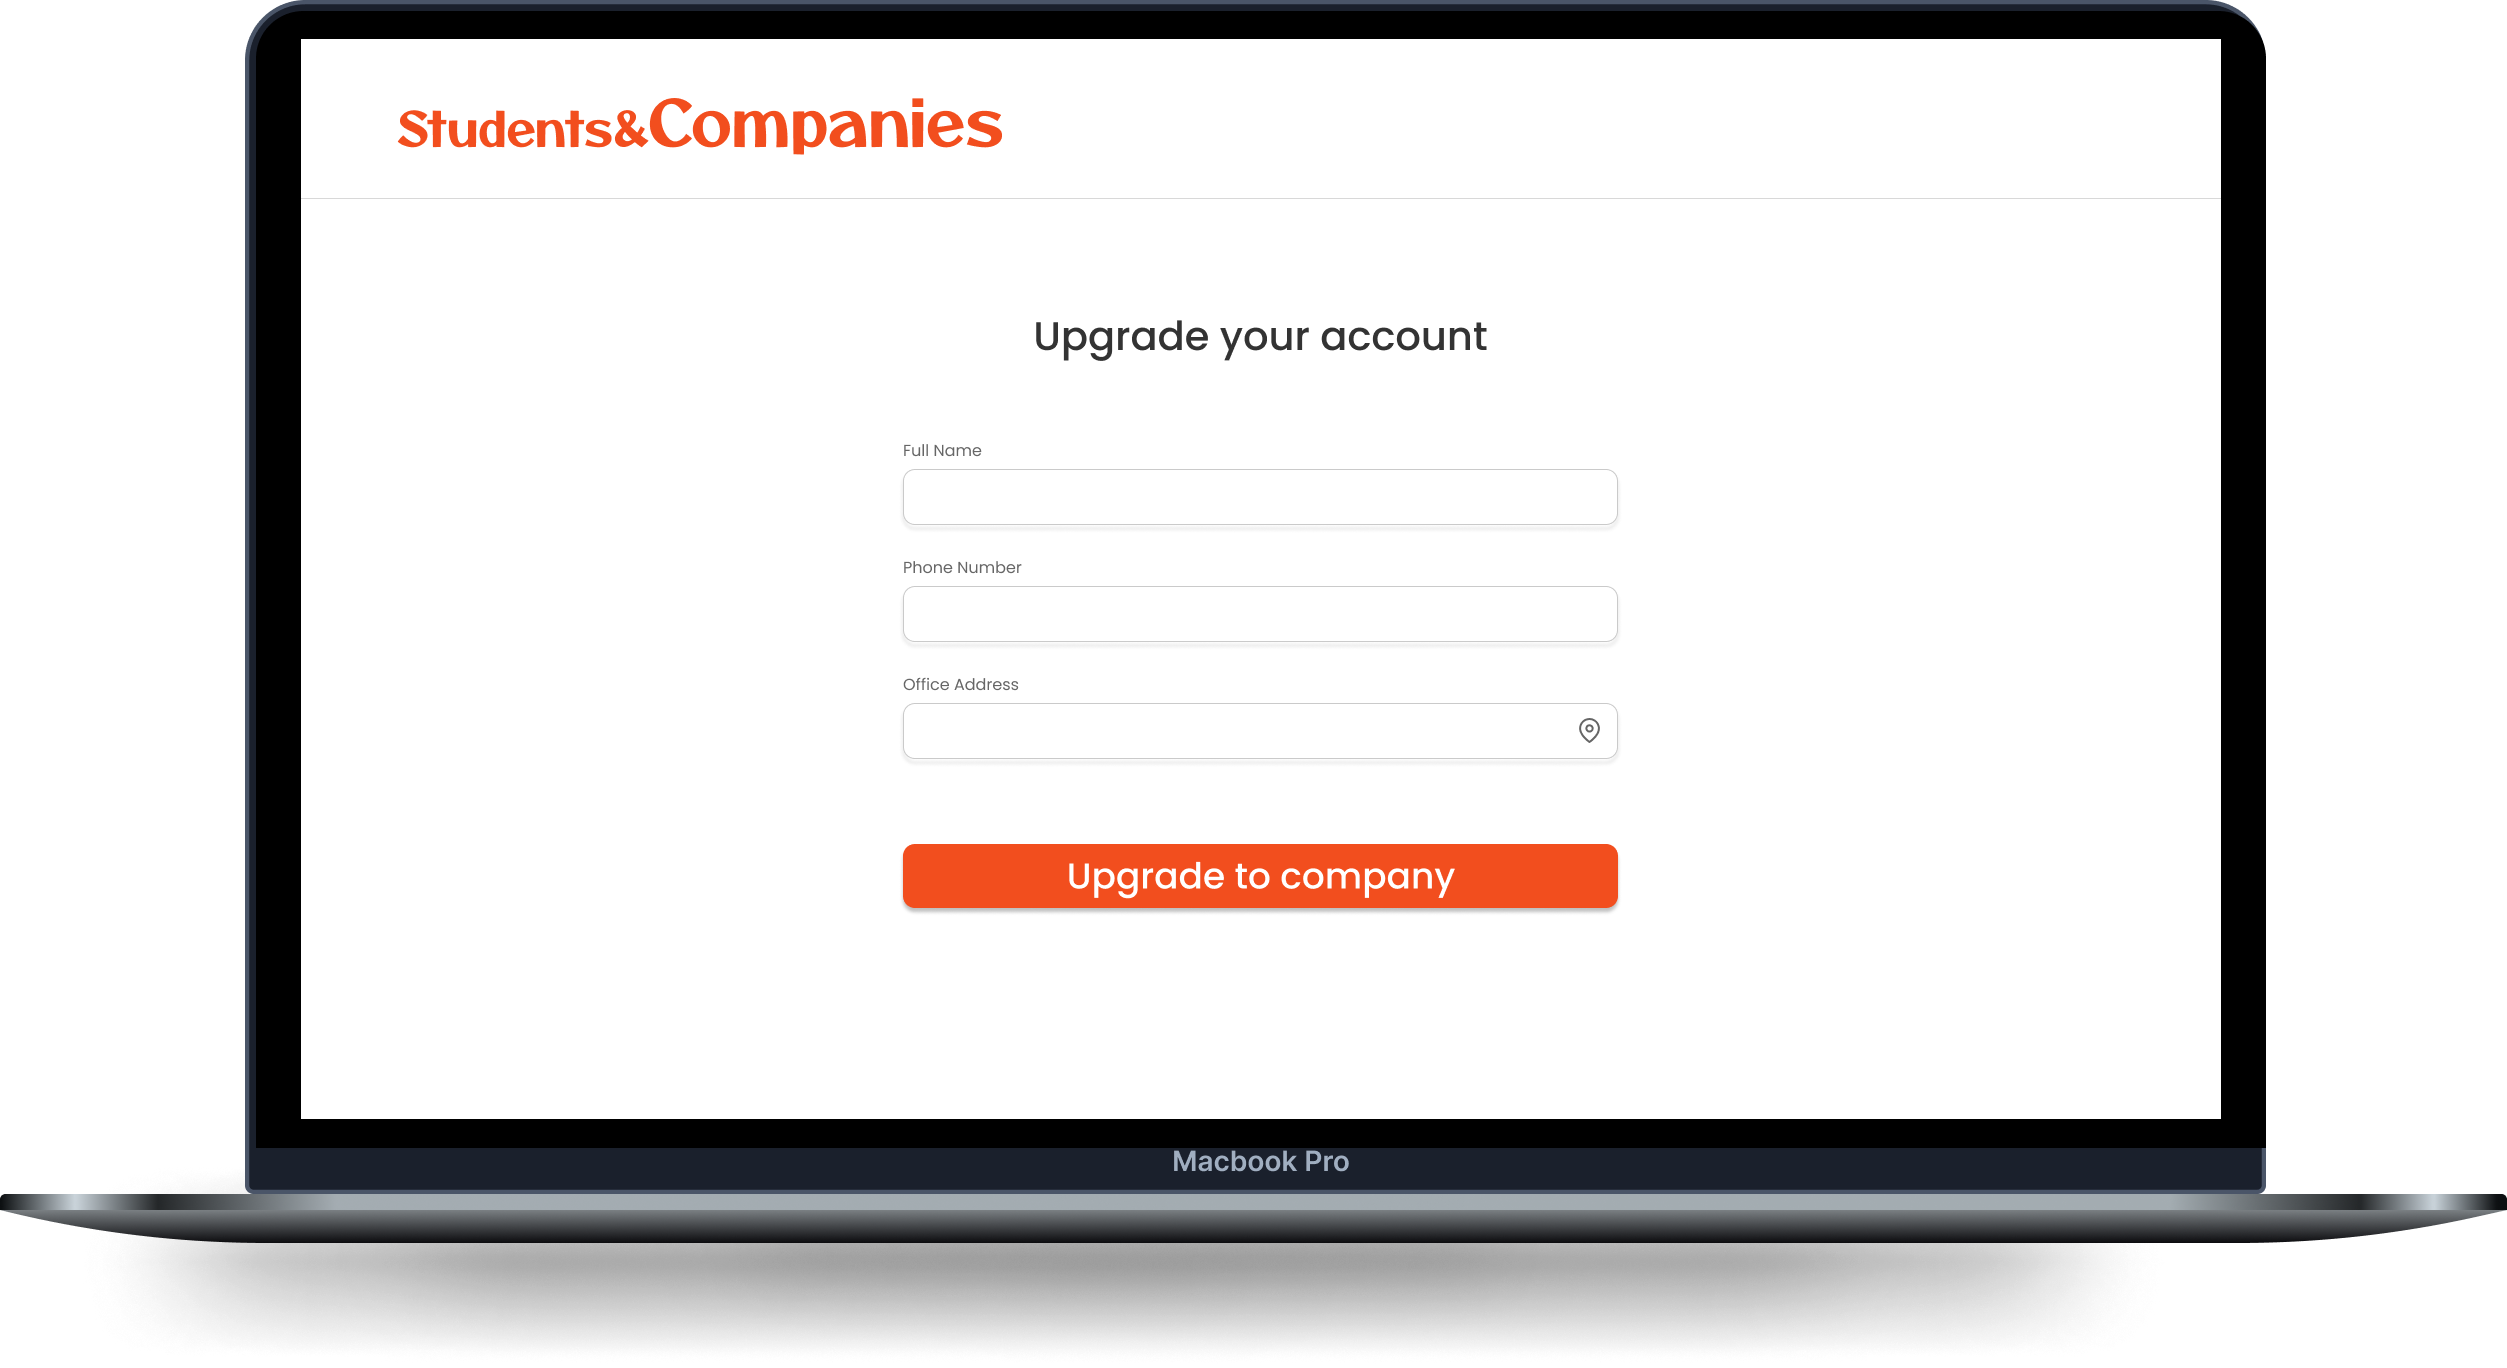
\includegraphics[width=0.75\linewidth]{Images/Mock-up/UpgradeToCompanyPC.png}
    \caption{S\&C Company Account Activation Page Design}
    \label{fig:homepage-design}
\end{figure}

\section{Student Dashboard Interface}

Students can access this page after logging in or activating their student account. On this page, they can browse all available internships. By default, internships are displayed in order of the highest compatibility, quantified by a score out of 10. The highest score, shown first, represents the best match. On this page the student can:

\begin{itemize}
    \item Open the Internship's details page by clicking an internship tab.
    \item Switch between available, active, applied, or terminated internships by using the sub-menu bar.
    \item Change the listing order (e.g., by distance or highest salary) by clicking the "sort" button.
    \item Apply filters to exclude posts based on specific characteristics (e.g., distance range, salary range) by clicking the "filter" button.
    \item Search for companies by name or requested role by typing it in the search bar.
    \item See all notifications by clicking on notification button.
    \item Open the edit profile page by clicking the profile picture or "profile" text. \\
\end{itemize}

\begin{figure}[H]
    \centering
    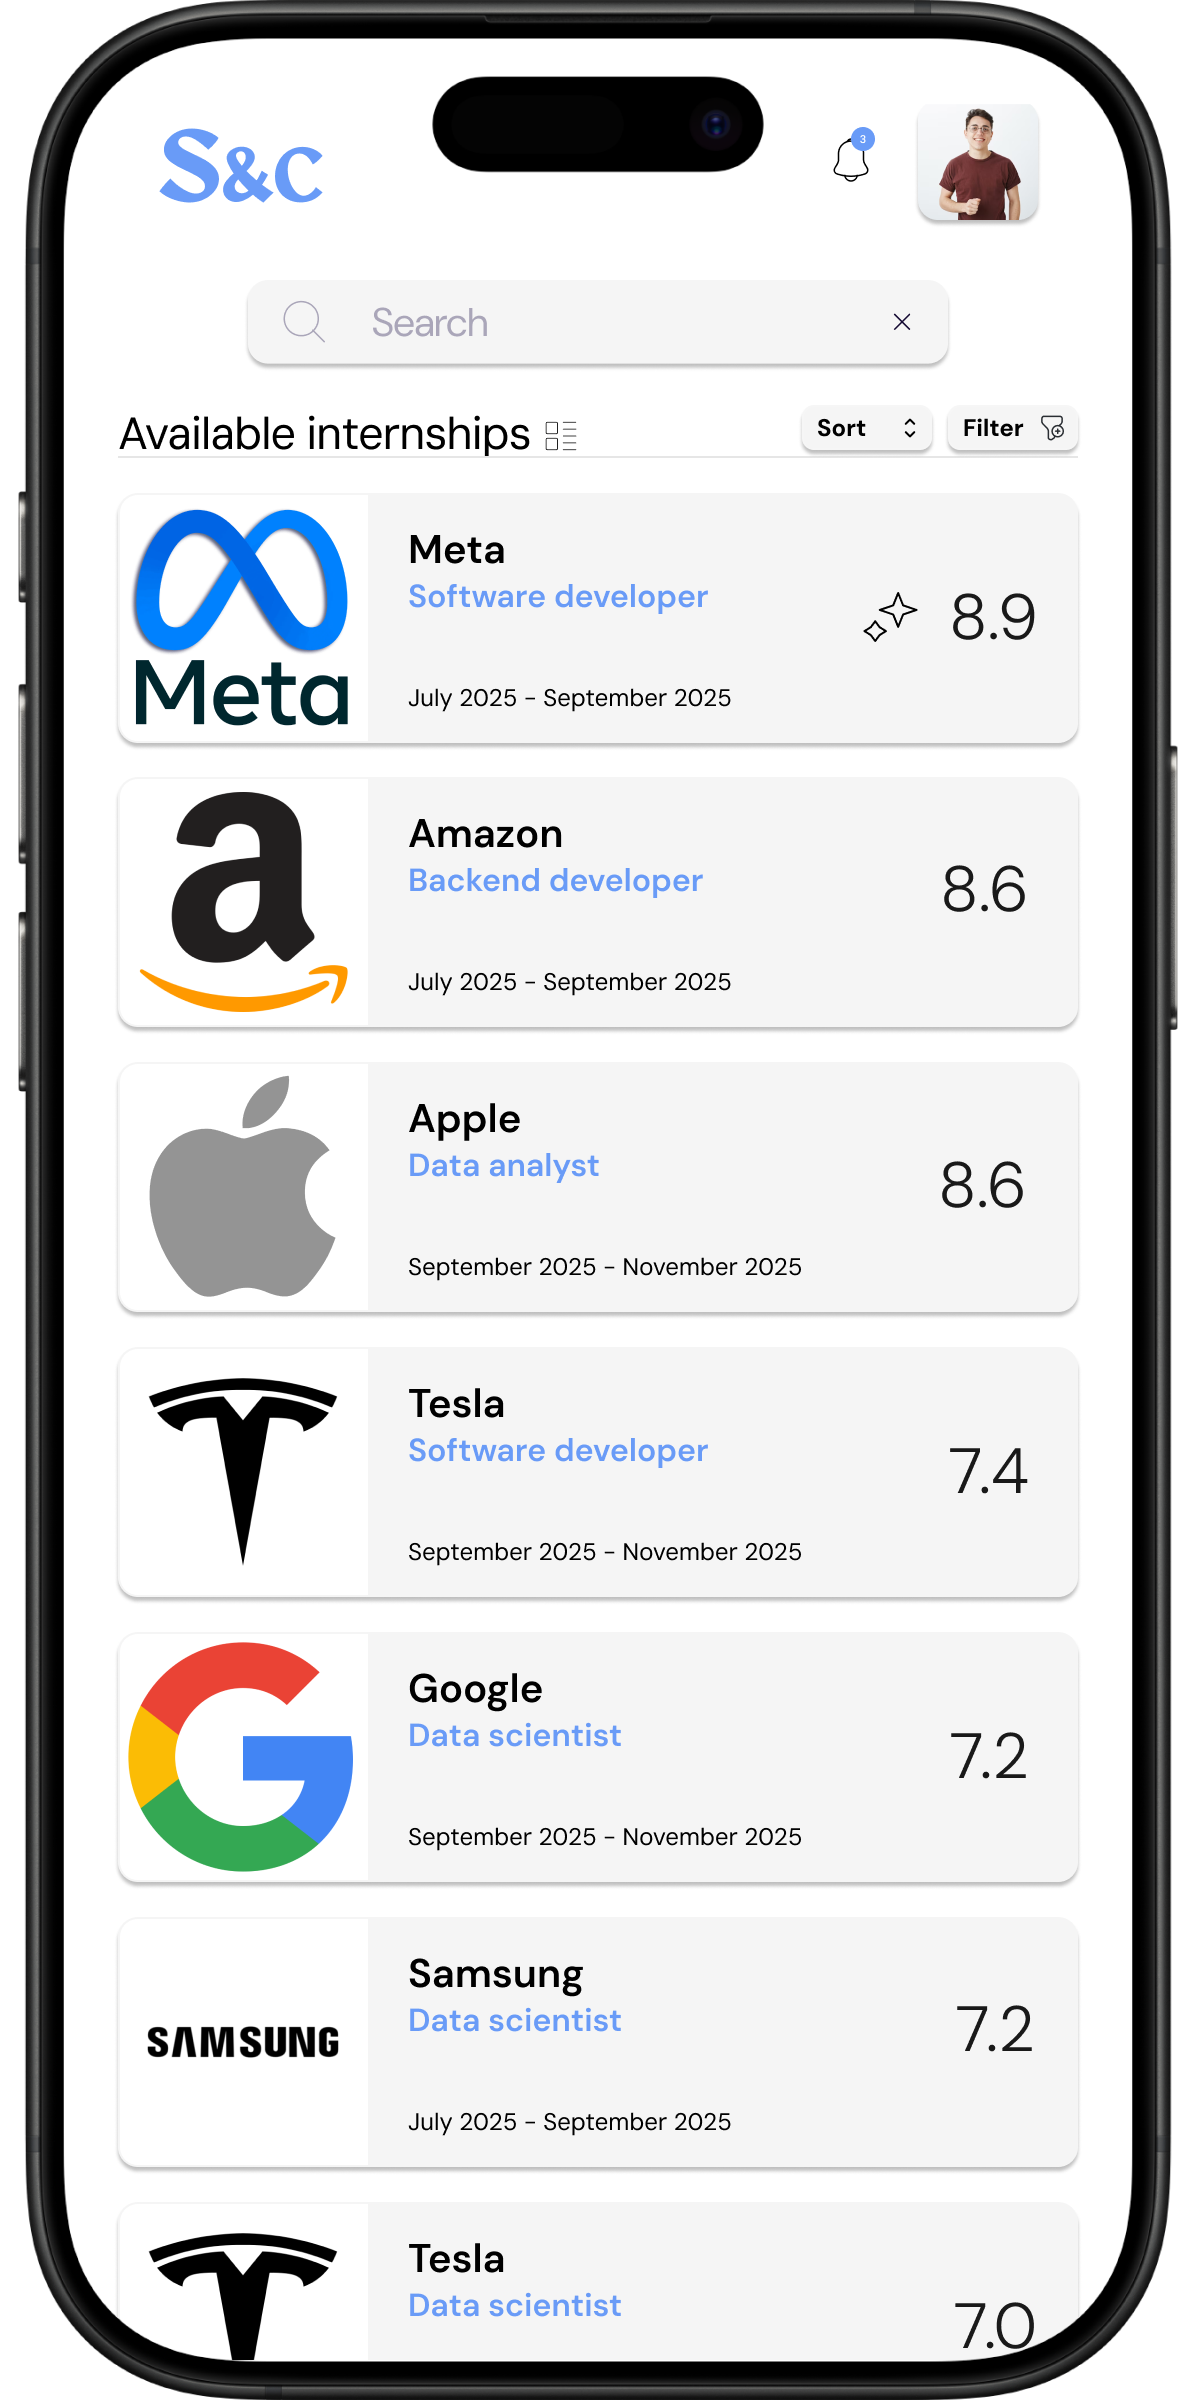
\includegraphics[width=0.2\linewidth]{Images/Mock-up/mobile homepage student.png}
    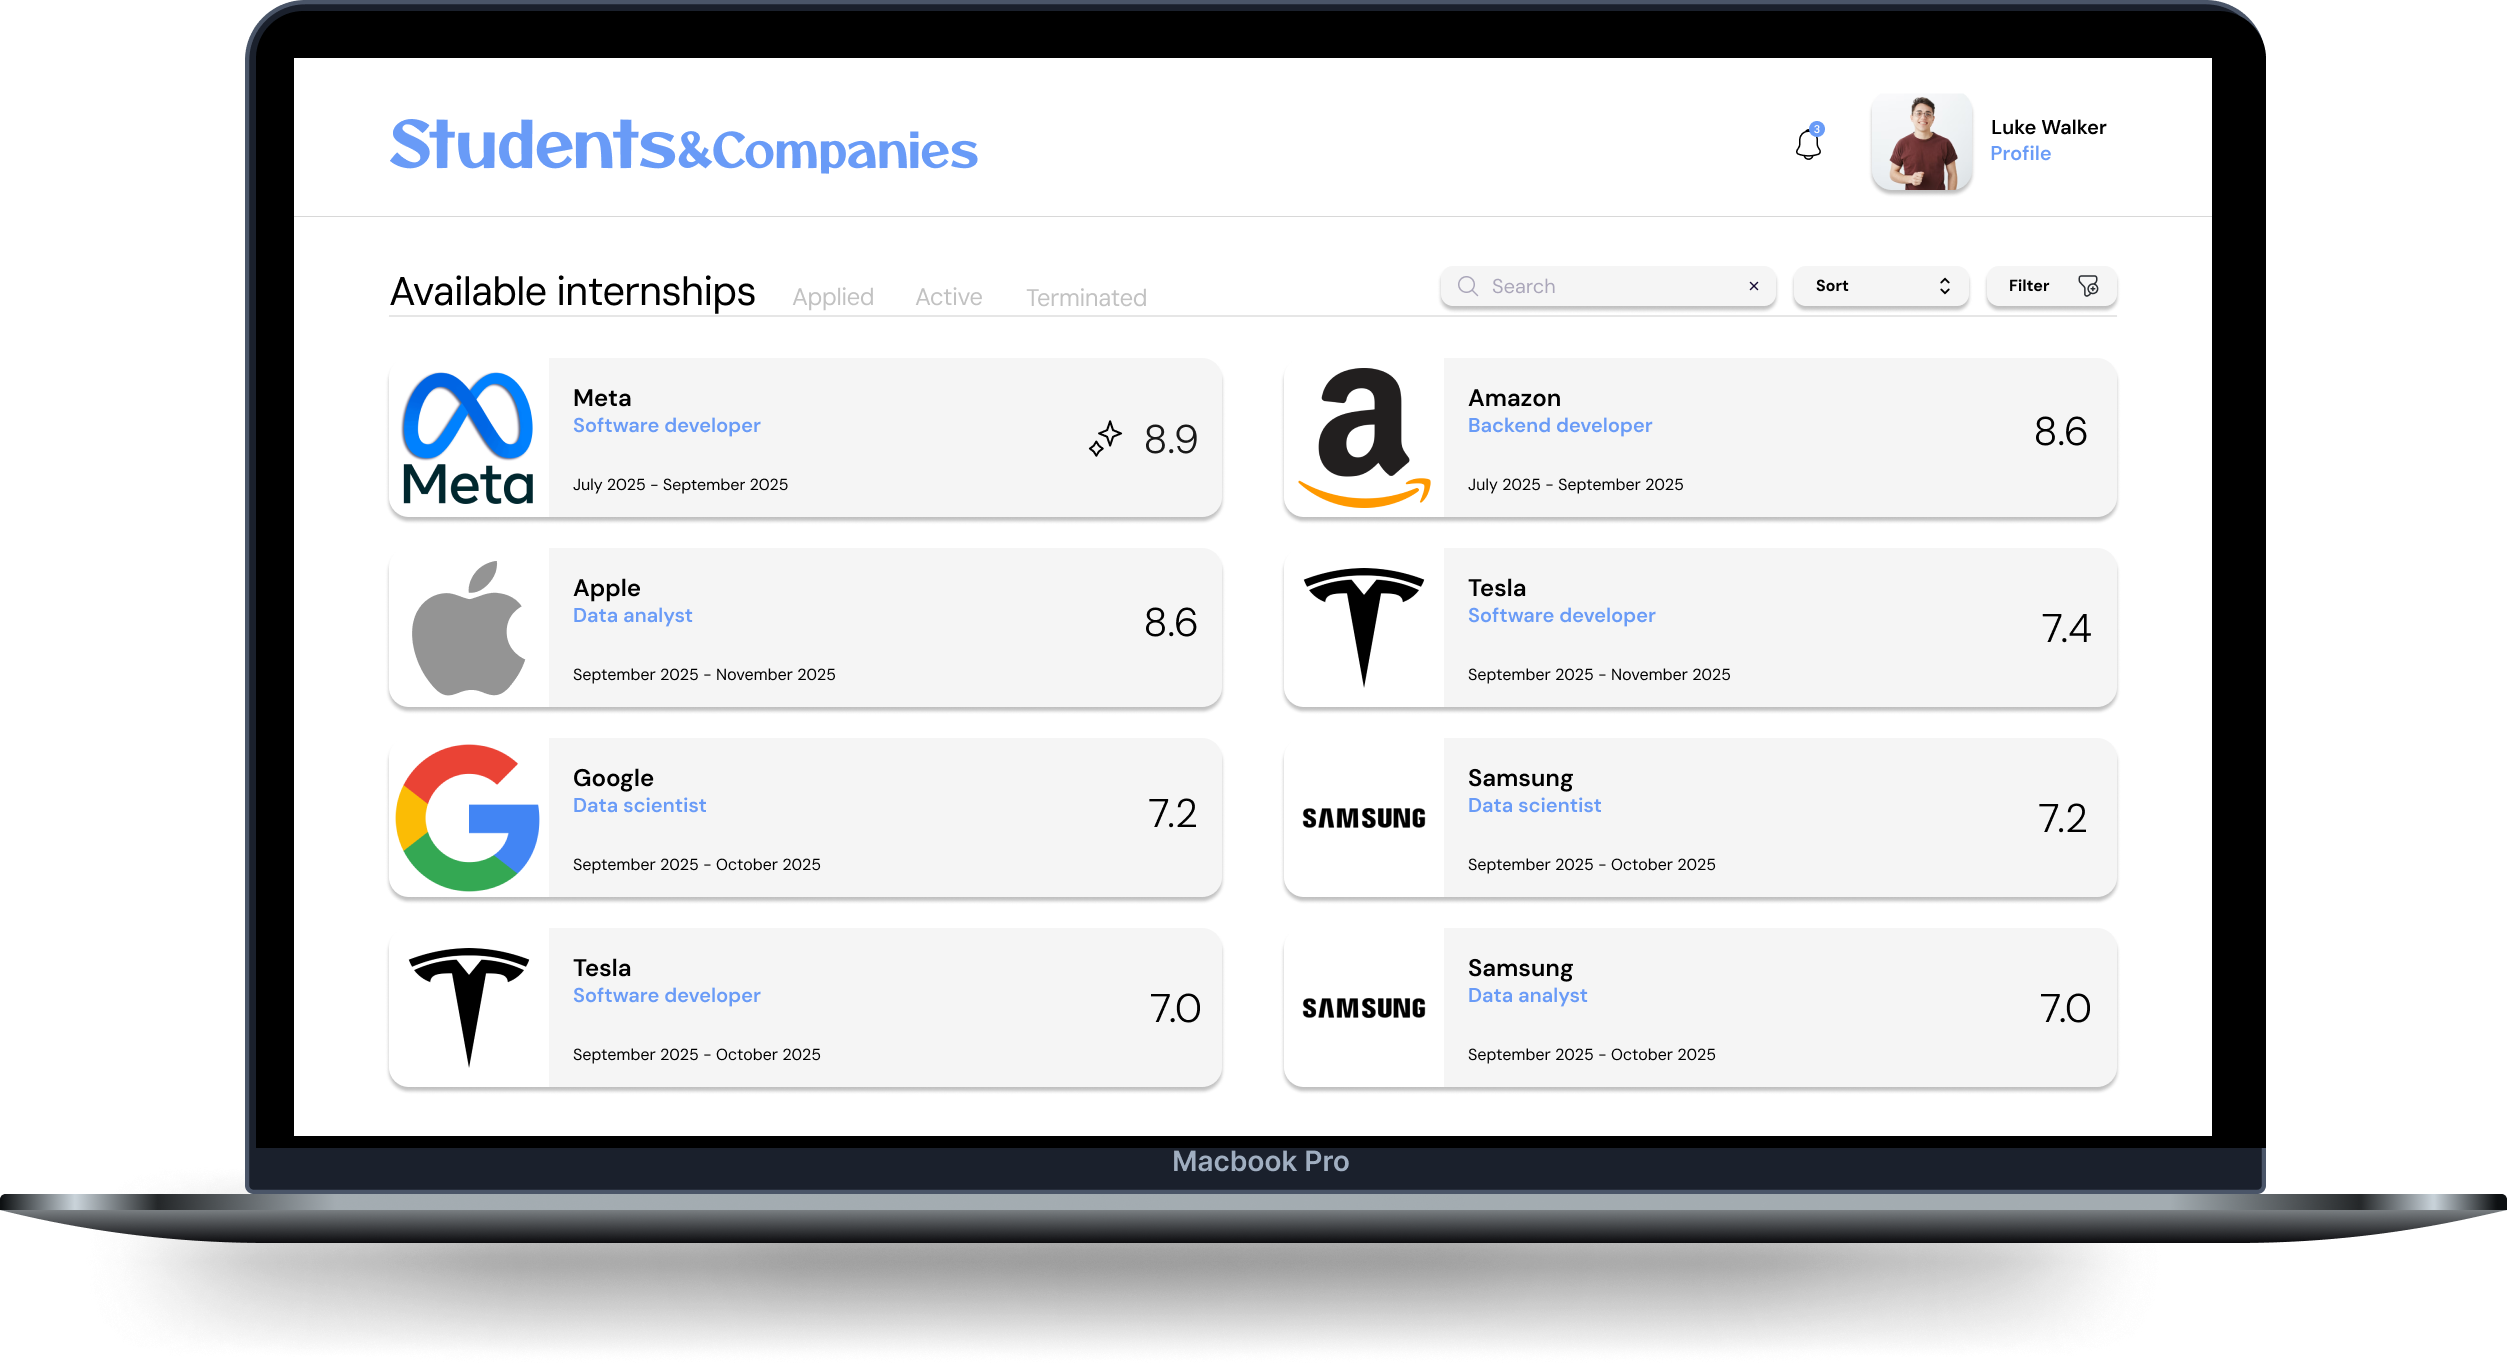
\includegraphics[width=0.75\linewidth]{Images/Mock-up/homepage student.png}
    \caption{S\&C Student Homepage Design}
    \label{fig:homepage-design}
\end{figure}
    

\subsection{Edit Profile Interface}

Students can access this page by clicking the profile picture or "Profile" text on their homepage. On this page, they can update their personal information by completing the desired fields in the form or upload a new CV file using the dedicated input field. The system provides personalized suggestions based on the current CV to enhance its appeal to companies and improve compatibility with the matching algorithm. Updating personal information and uploading a new CV are independent actions. Changes are submitted to the system only after clicking the confirmation button. Students can also navigate back to the homepage without saving any changes. \\

\begin{figure}[H]
    \centering
    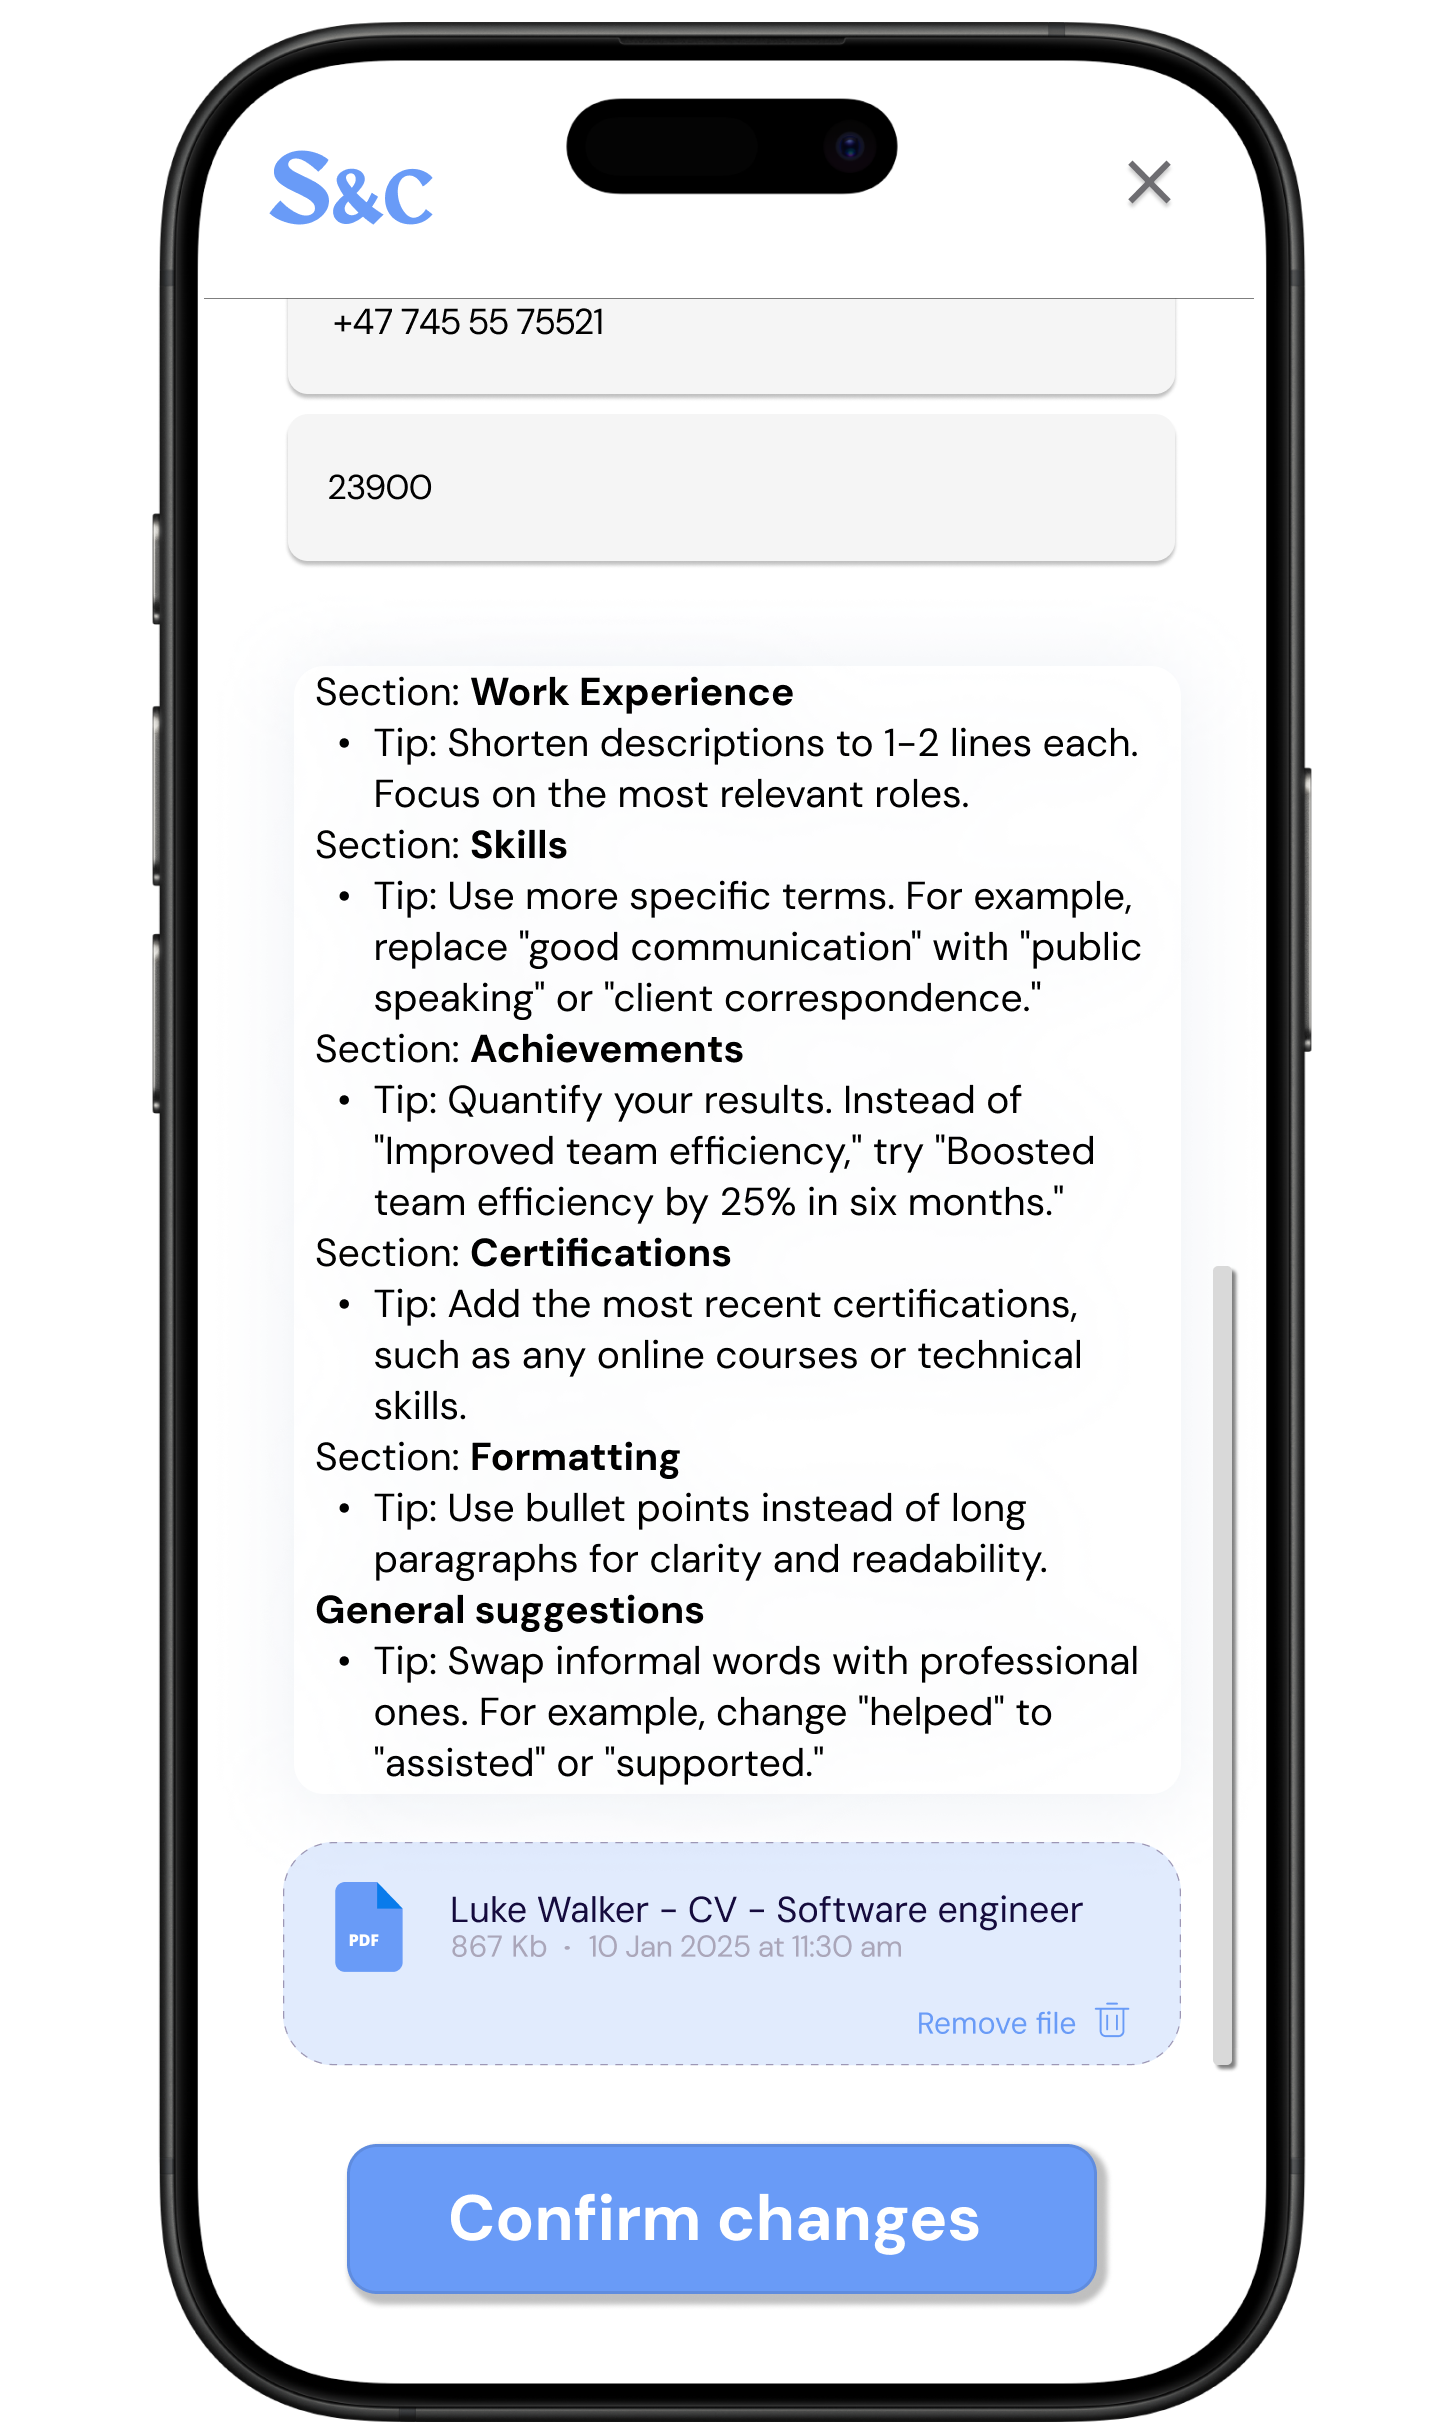
\includegraphics[width=0.2\linewidth]{Images/Mock-up/EditProfileMobile.png}
    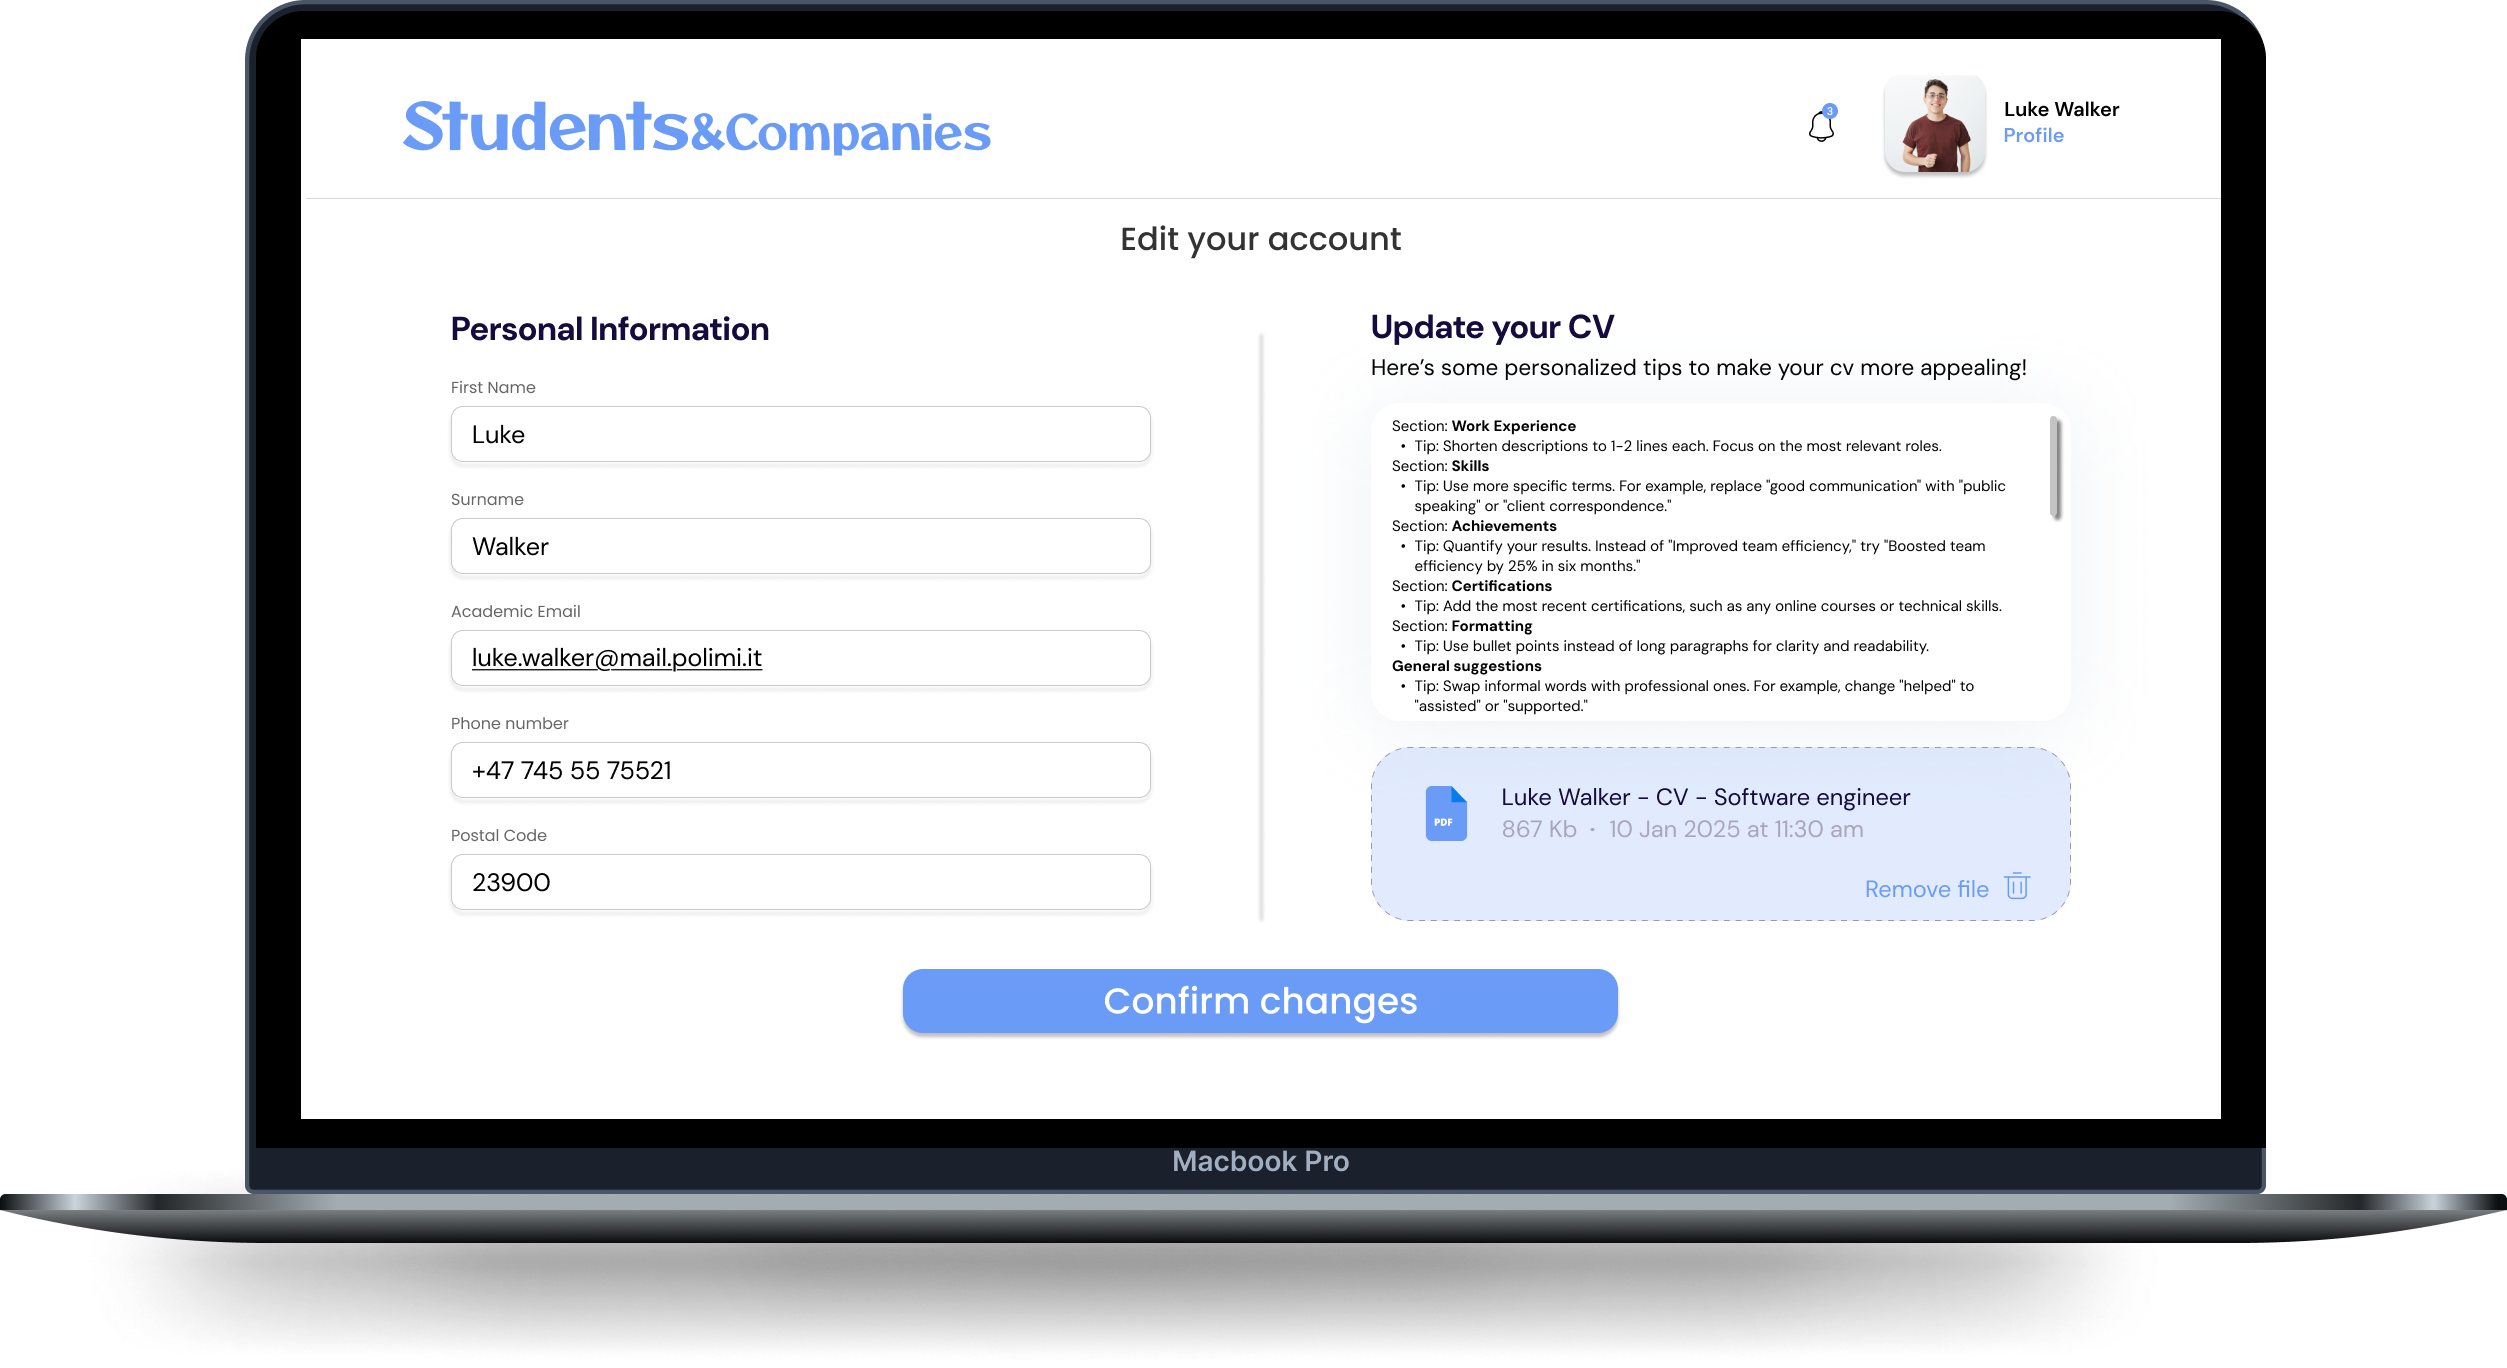
\includegraphics[width=0.75\linewidth]{Images/Mock-up/EditProfilePC.png}
    \caption{S\&C Internship Details Design}
    \label{fig:homepage-design}
\end{figure}

\subsection{Internship Details Interface}
Students can access this page by clicking on one of the internship offer boxes on their homepage. On this page, they can read all the details about the internship and, if interested, decide to submit their application by clicking the respective button. This action will send a notification to the company, which can then choose whether to accept it or not. The details are displayed on the right half of the page, so students can directly view other internship offers by clicking on another box, as their list remains open on the left half. After clicking the submit application button, the student is brought back to their homepage. \\

\begin{figure}[H]
    \centering
    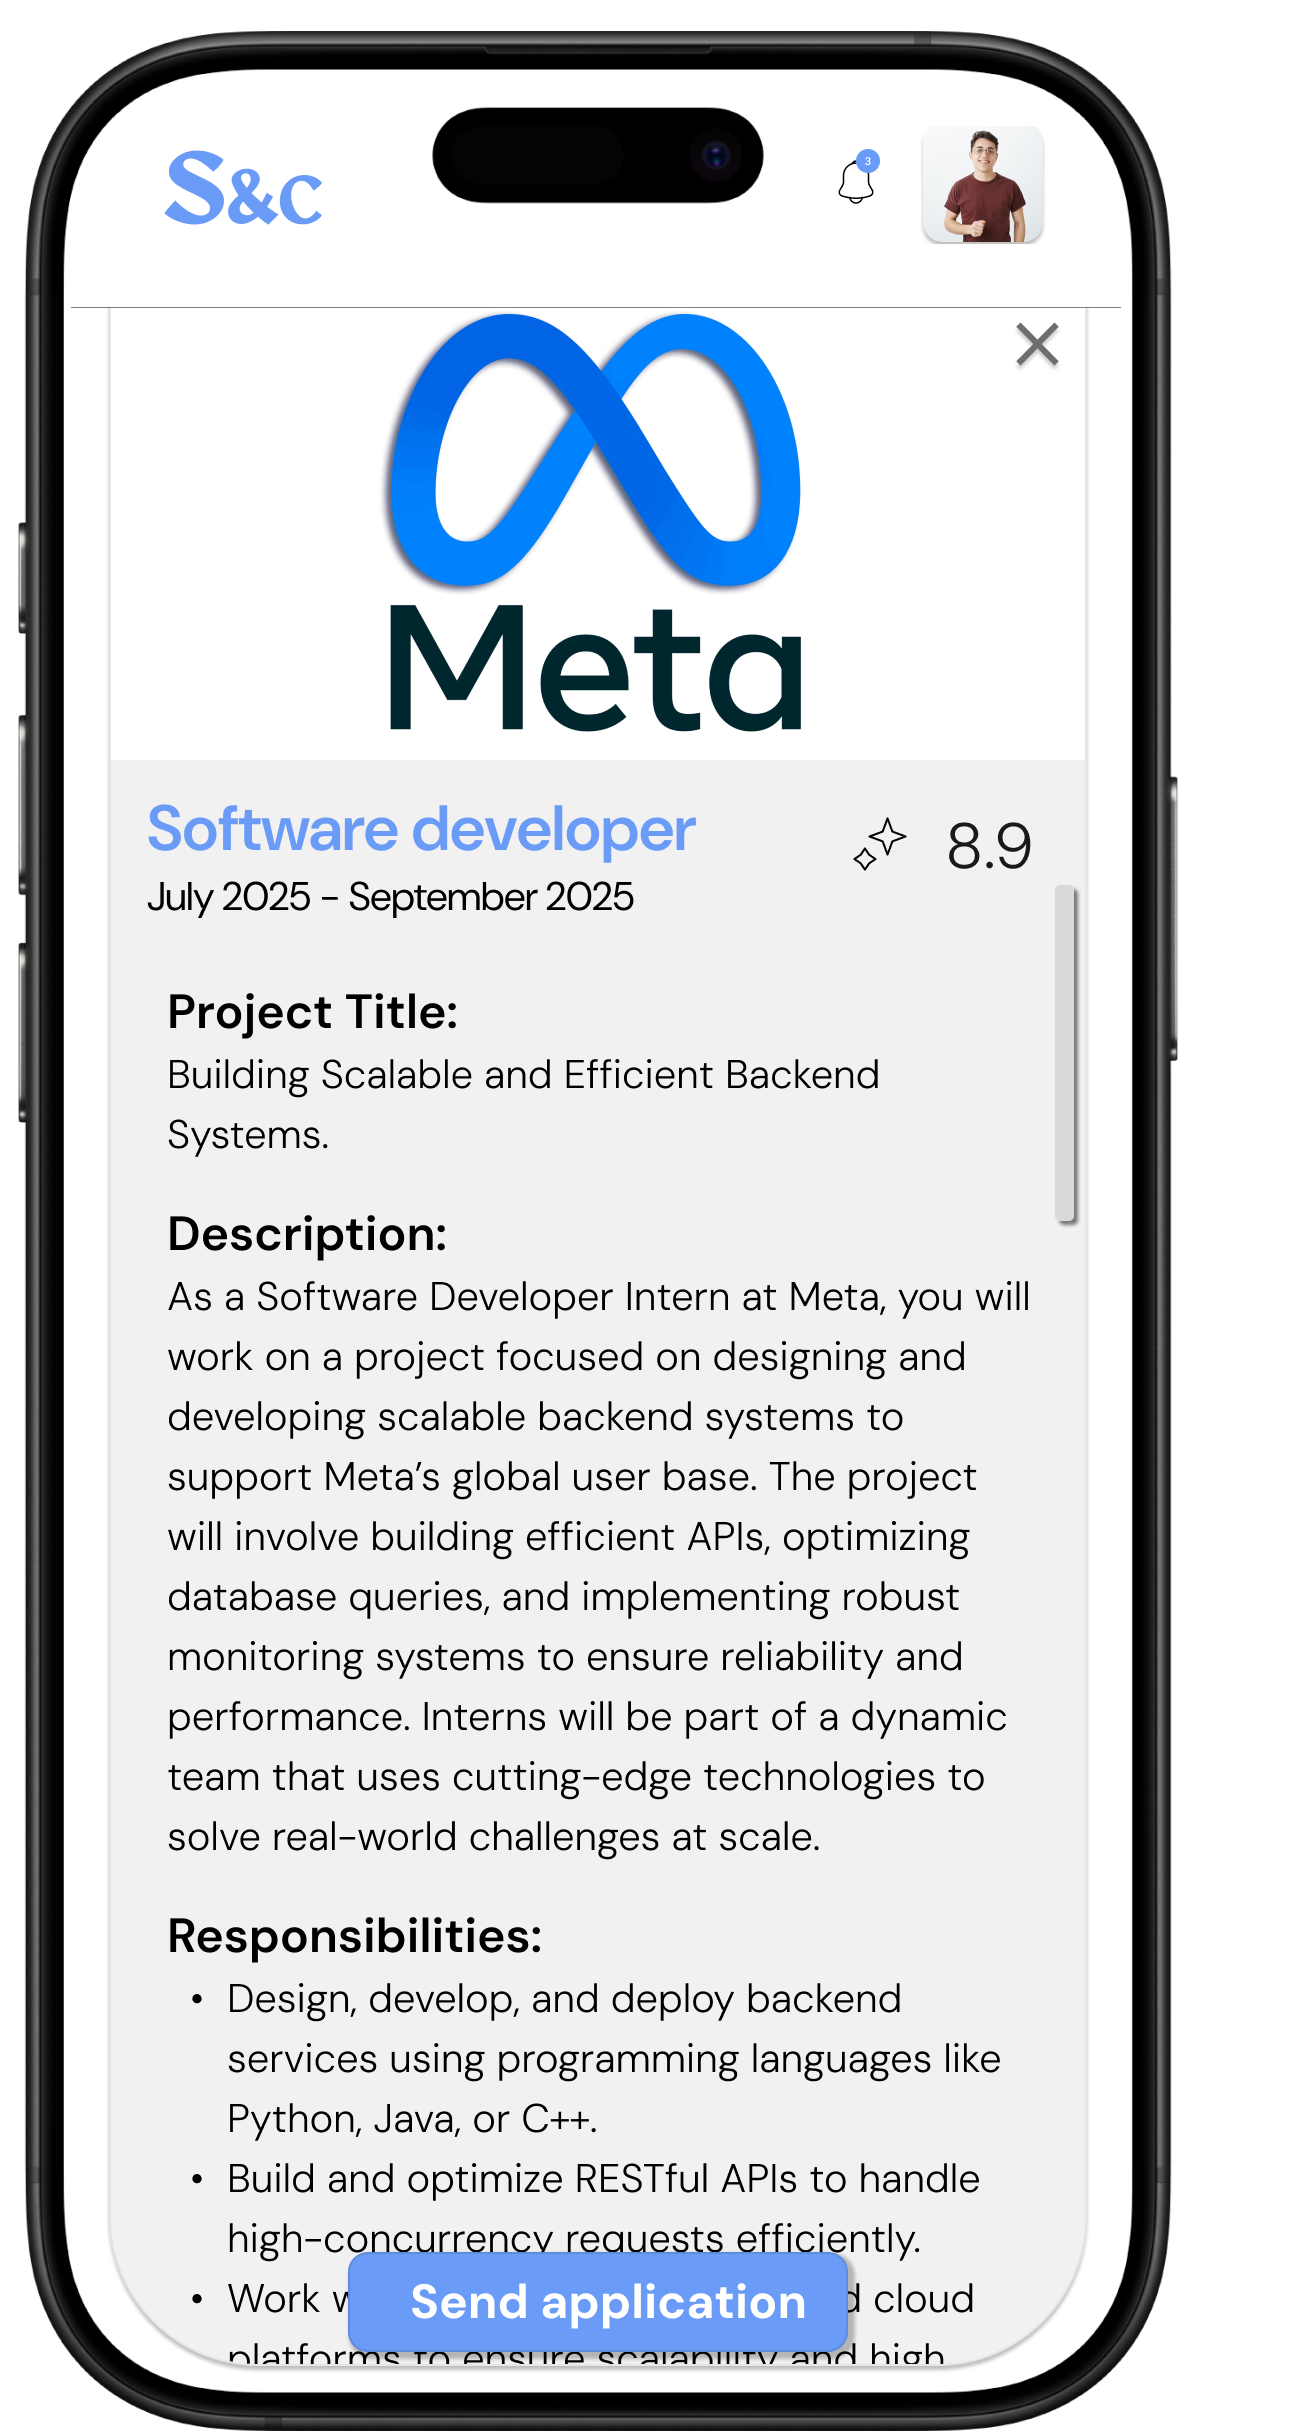
\includegraphics[width=0.2\linewidth]{Images/Mock-up/mobile nternship details.png}
    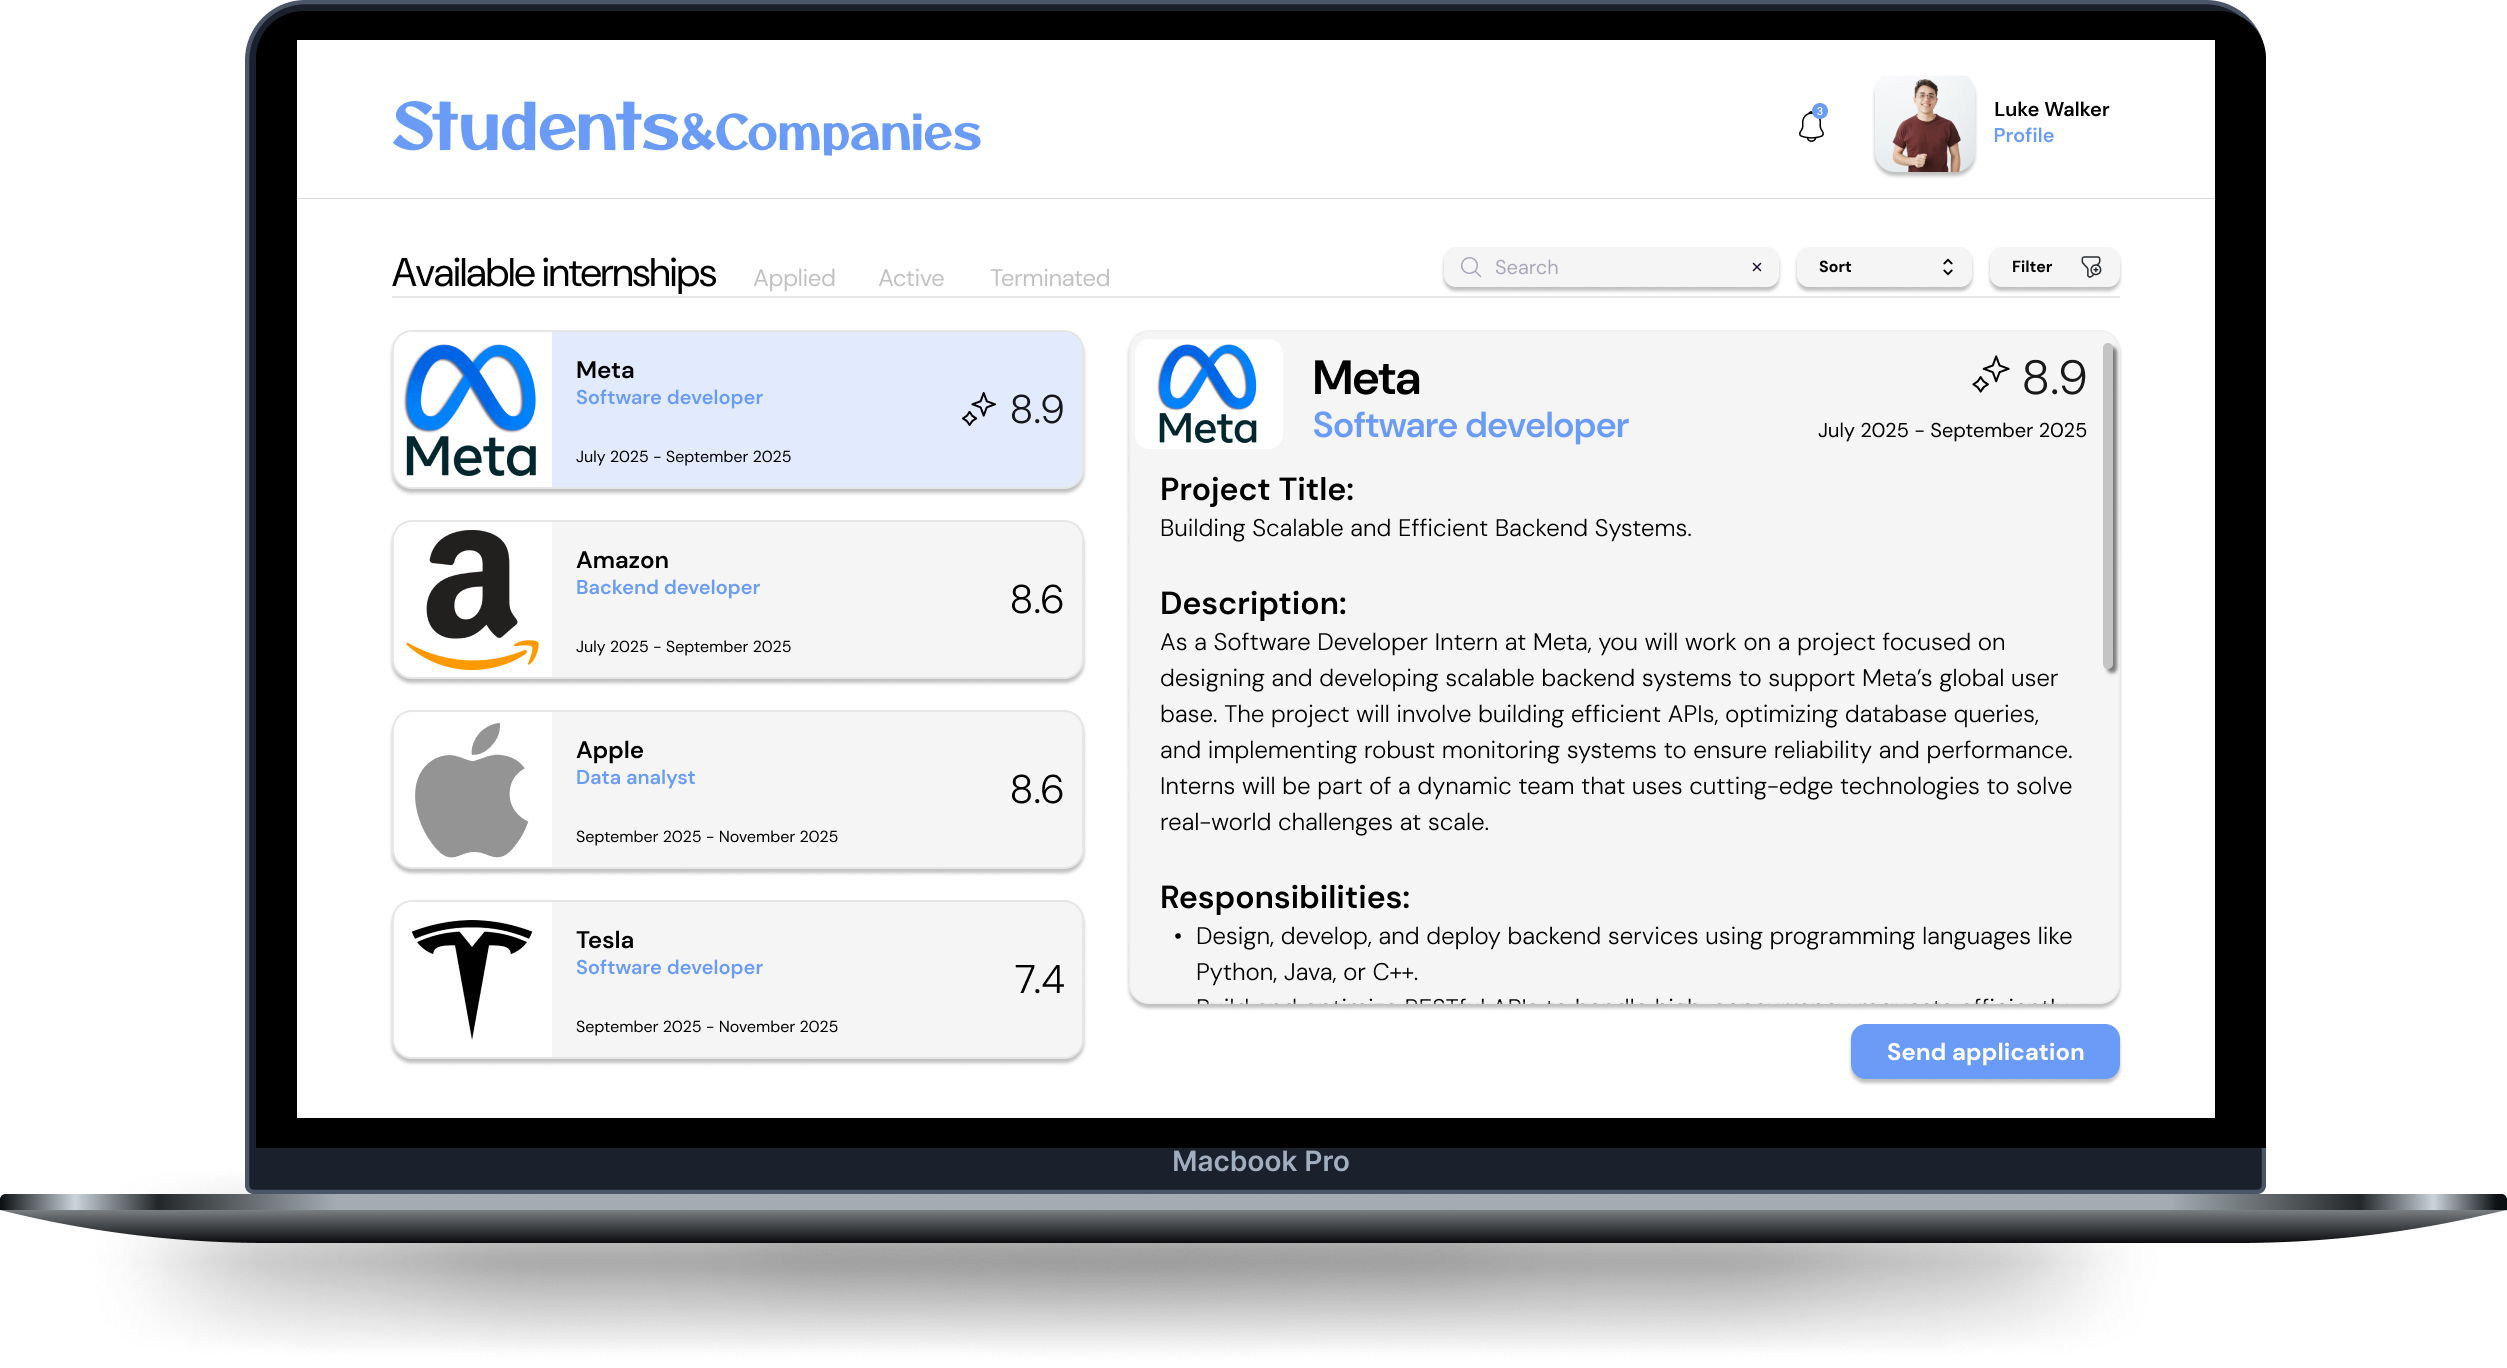
\includegraphics[width=0.75\linewidth]{Images/Mock-up/internship details.png}
    \caption{S\&C internship details design}
    \label{fig:homepage-design}
\end{figure}

\subsection{Submit a Complaint/Feedback Interface}

Students can access this page by clicking the "Make a Complaint" button after opening the details of an ongoing Internship in the "Active Internships" section of their homepage. On this page, they can review the internship details agreed upon before starting and submit a complaint by completing all the required fields in the form. Alternatively, they can return to the homepage without taking any action. \\

\begin{figure}[H]
    \centering
    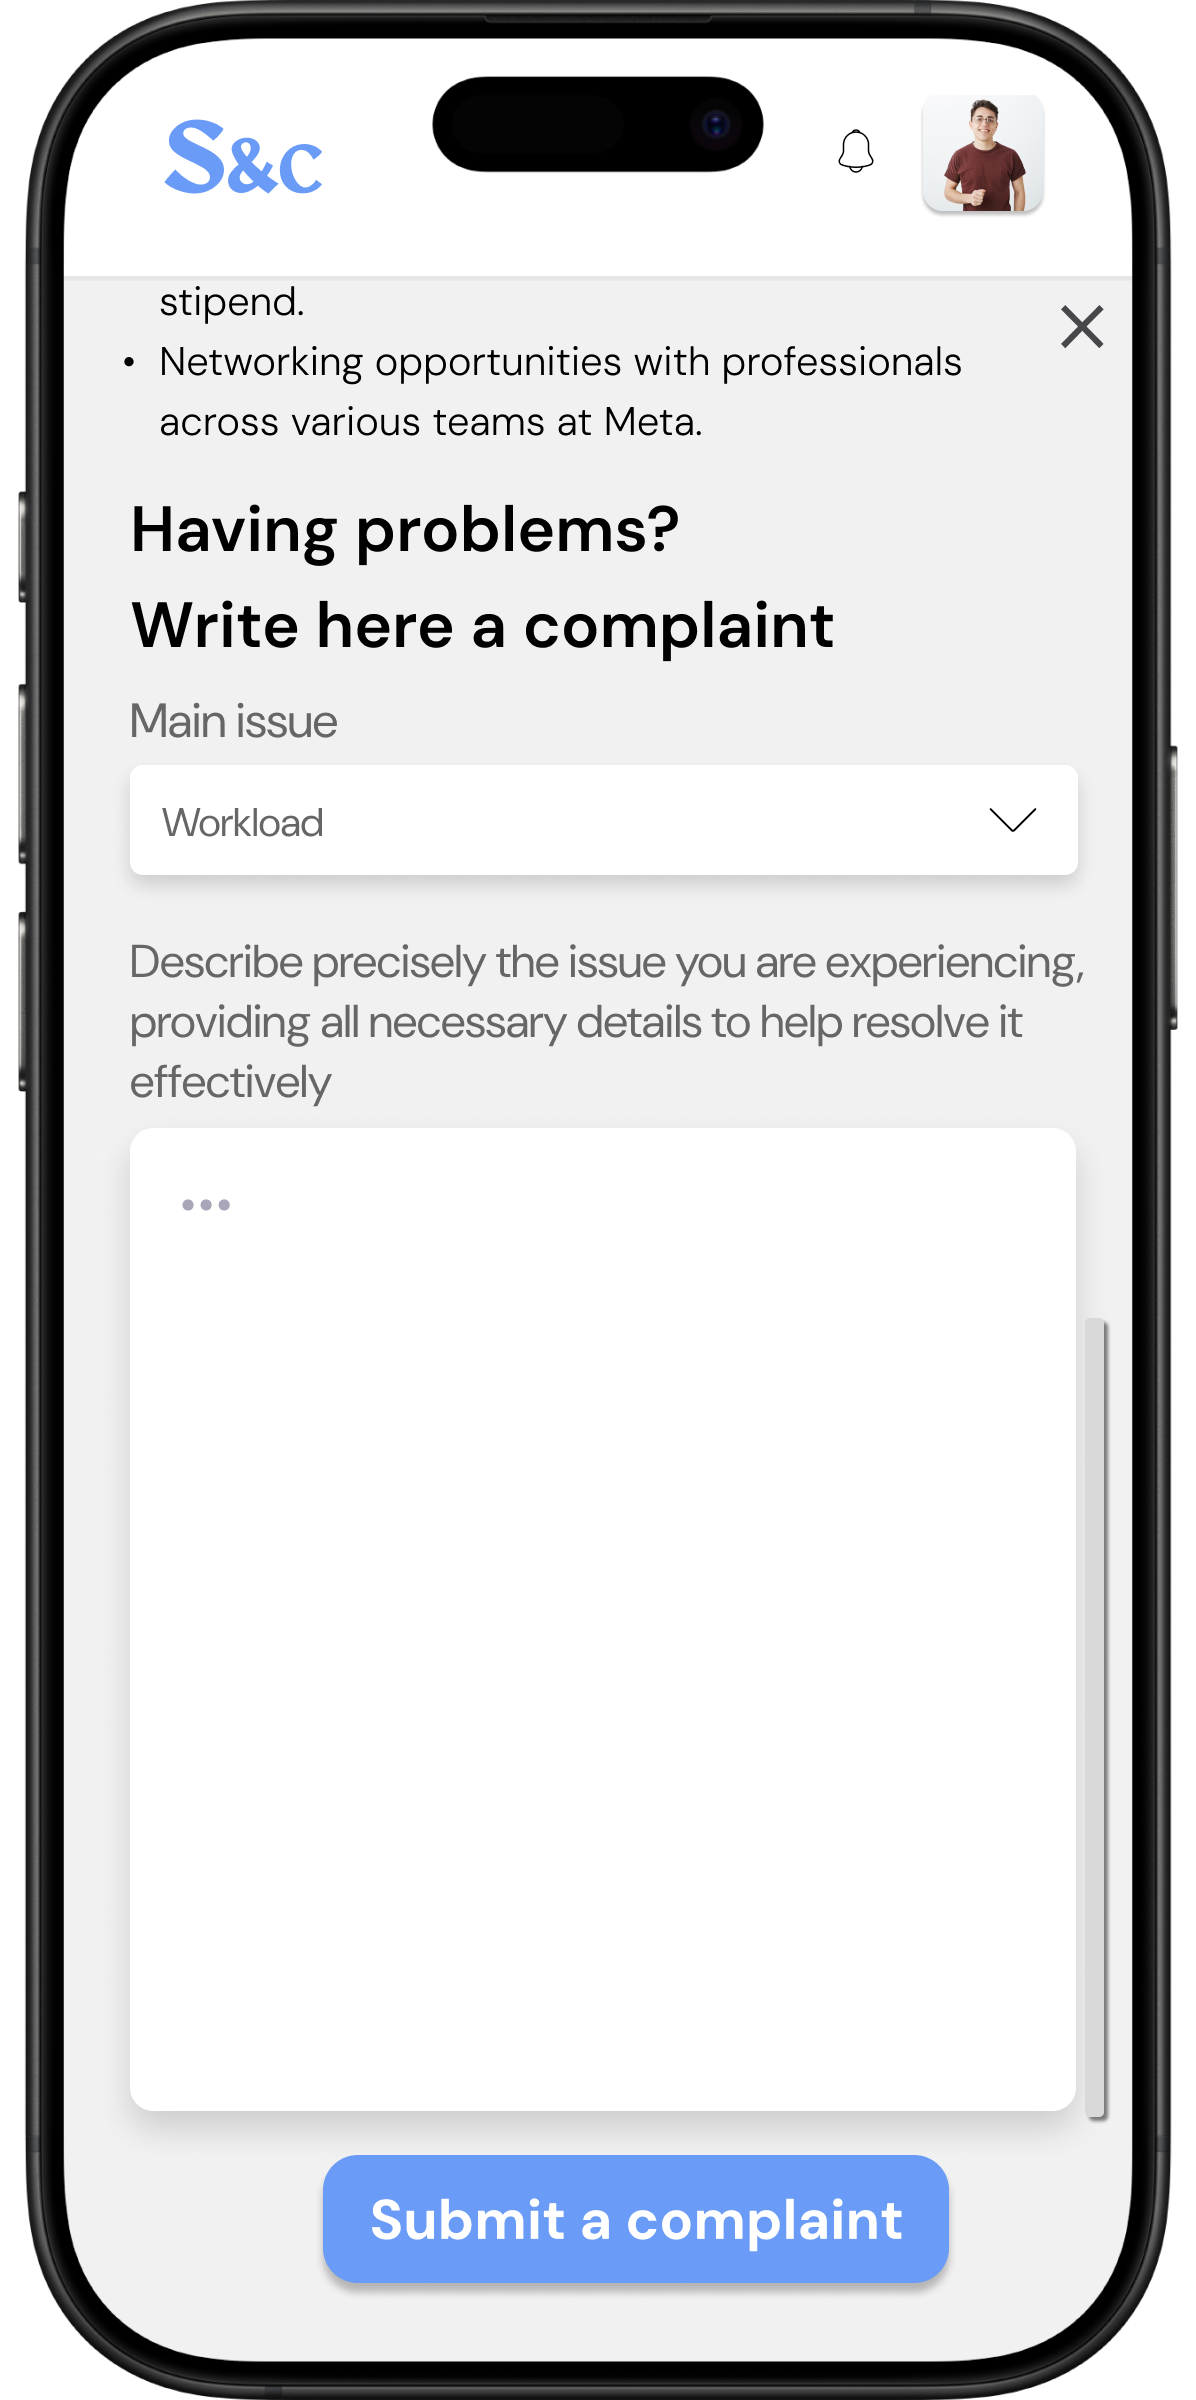
\includegraphics[width=0.2\linewidth]{Images/Mock-up/ComplaintMobile.png}
    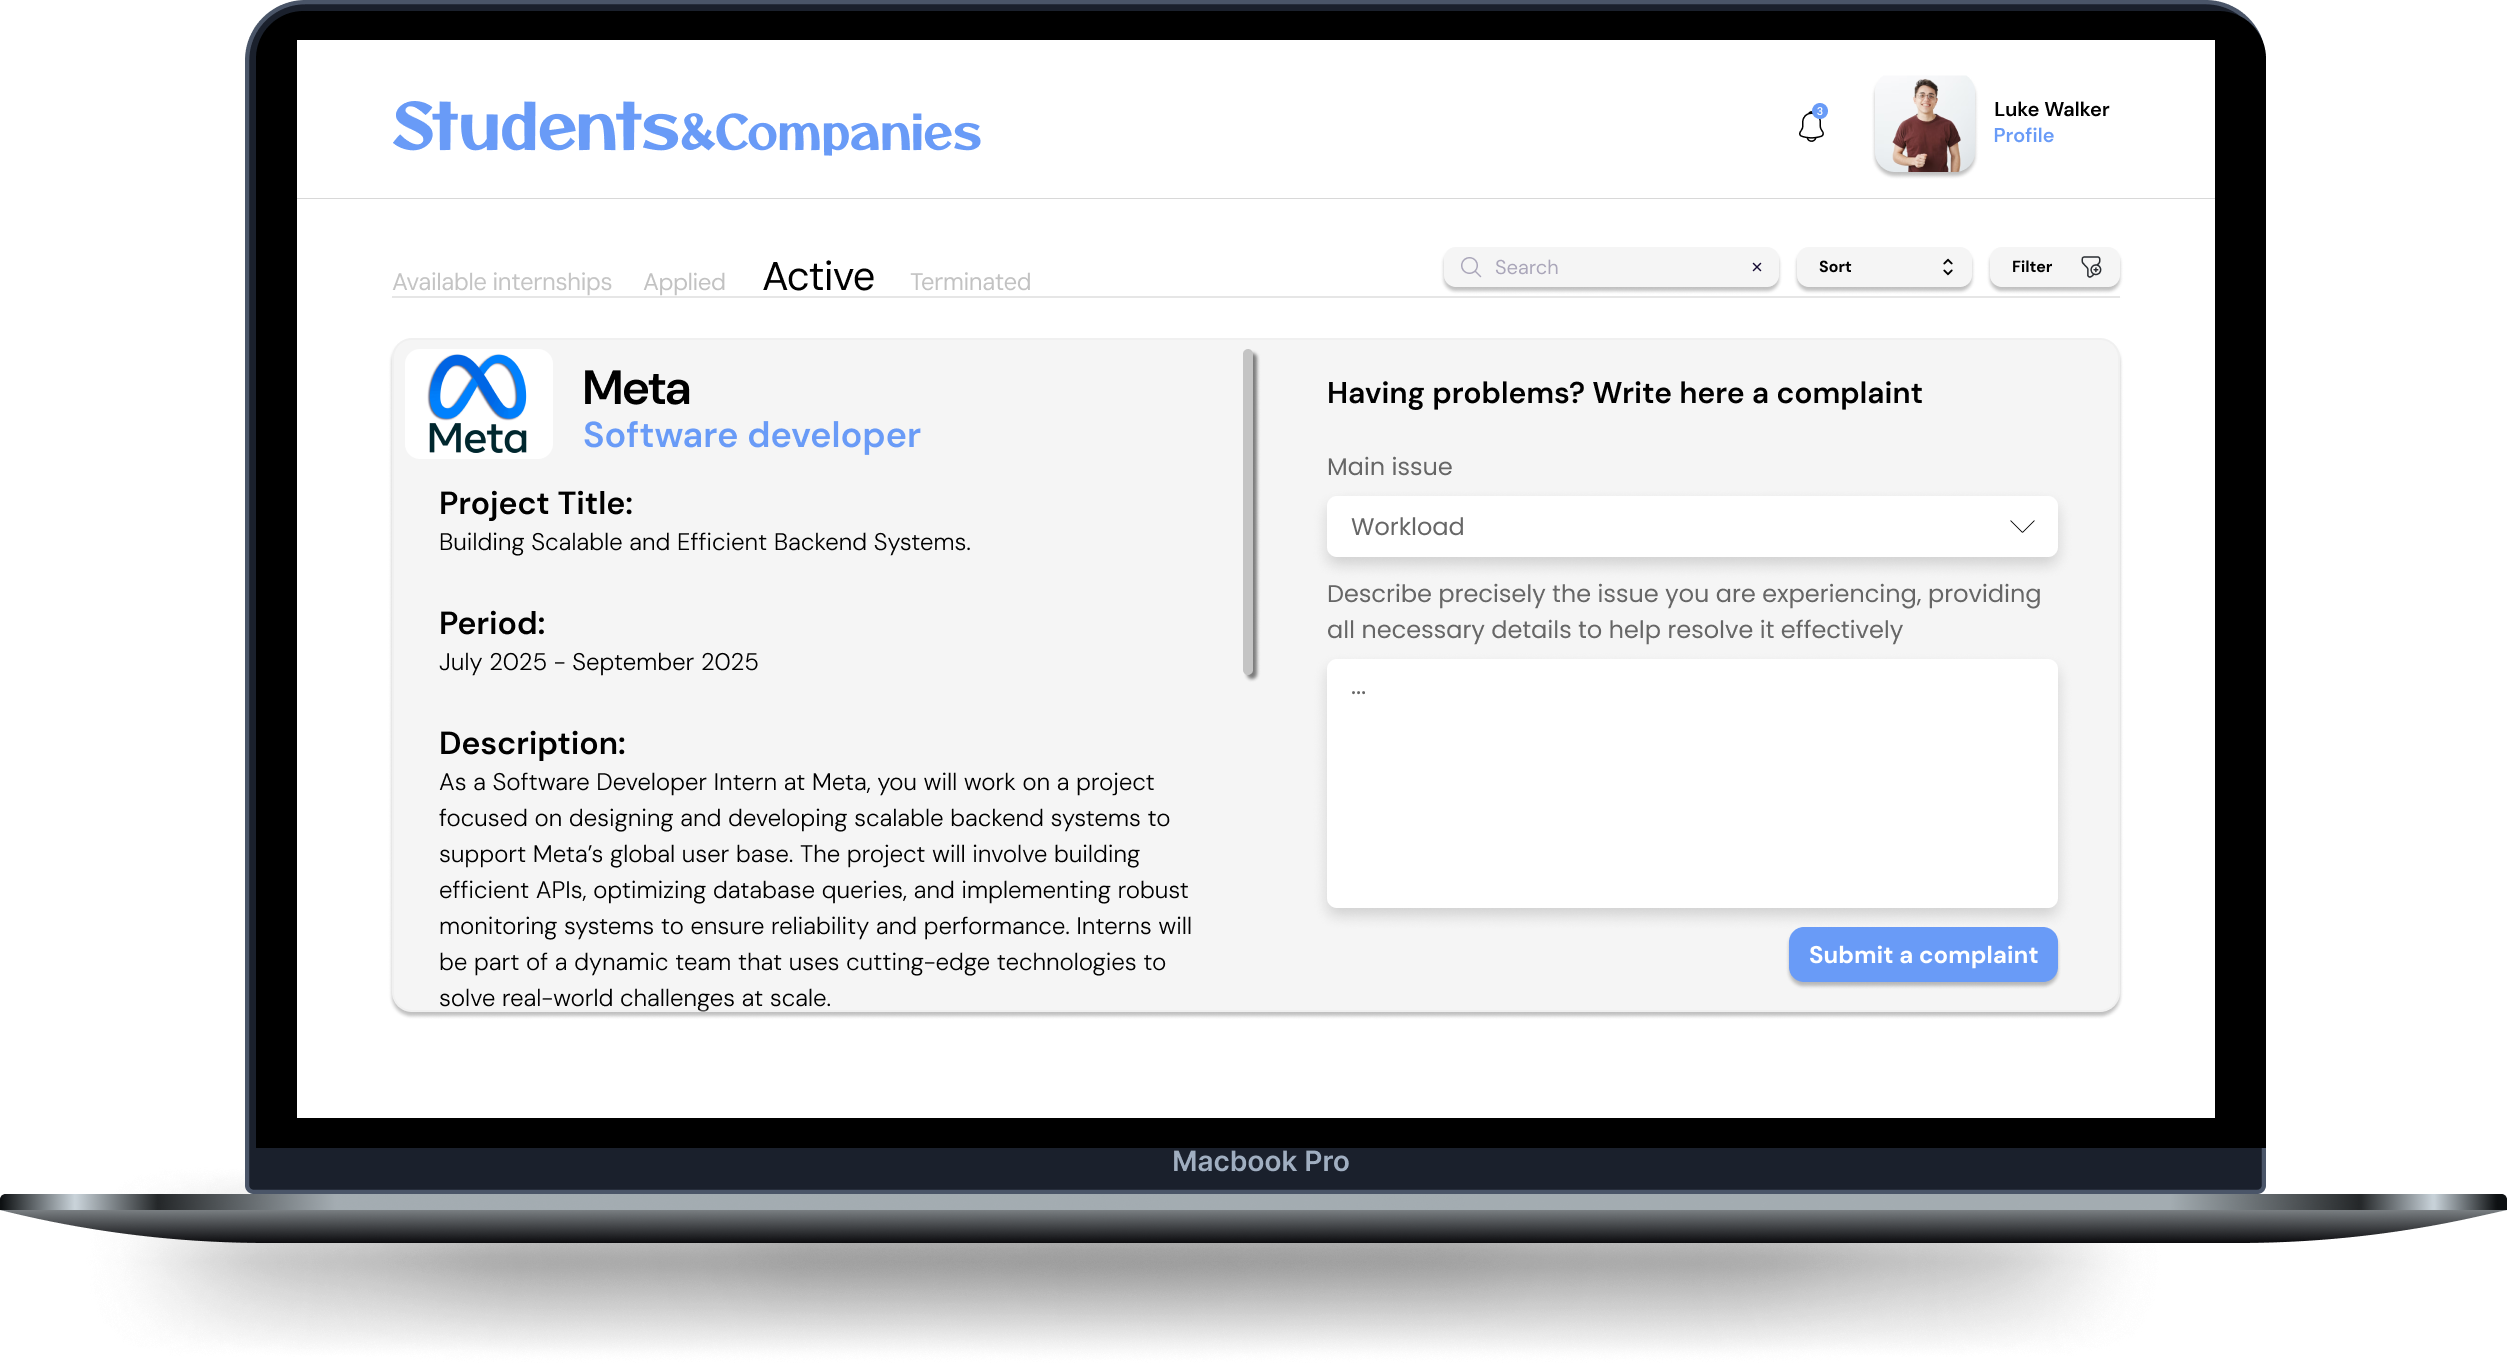
\includegraphics[width=0.75\linewidth]{Images/Mock-up/complaint.png}
    \caption{S\&C Submit a Complaint Page Design}
    \label{fig:homepage-design}
\end{figure}

\section{Company interface}

Companies can access this page after logging in or activating their company account. On this page, they can review all their posted internships. On this page, they can also:
\begin{itemize} 
    \item Open the details of an Internship by clicking its tab.
    \item Open the details of an Internship for modifications by clicking the edit button on its tab.
    \item Open the candidates page for an Internship by clicking the "Find Students" button on its tab opens.
    \item Switch between posted, active, or terminated internships by using the sub-menu bar.
    \item Change the listing order (e.g., by name or date) by clicking on the "sort" button.
    \item Apply filters to exclude posts based on specific characteristics (e.g., role requested, salary range) by clicking on the "filter" button.
    \item Searching for internships by role name by typing it in the search bar.
    \item Display all notifications by clicking on the notifications button.
    \item Open the edit profile page by clicking the profile picture or profile text. \\
\end{itemize}

\begin{figure}[H]
    \centering
    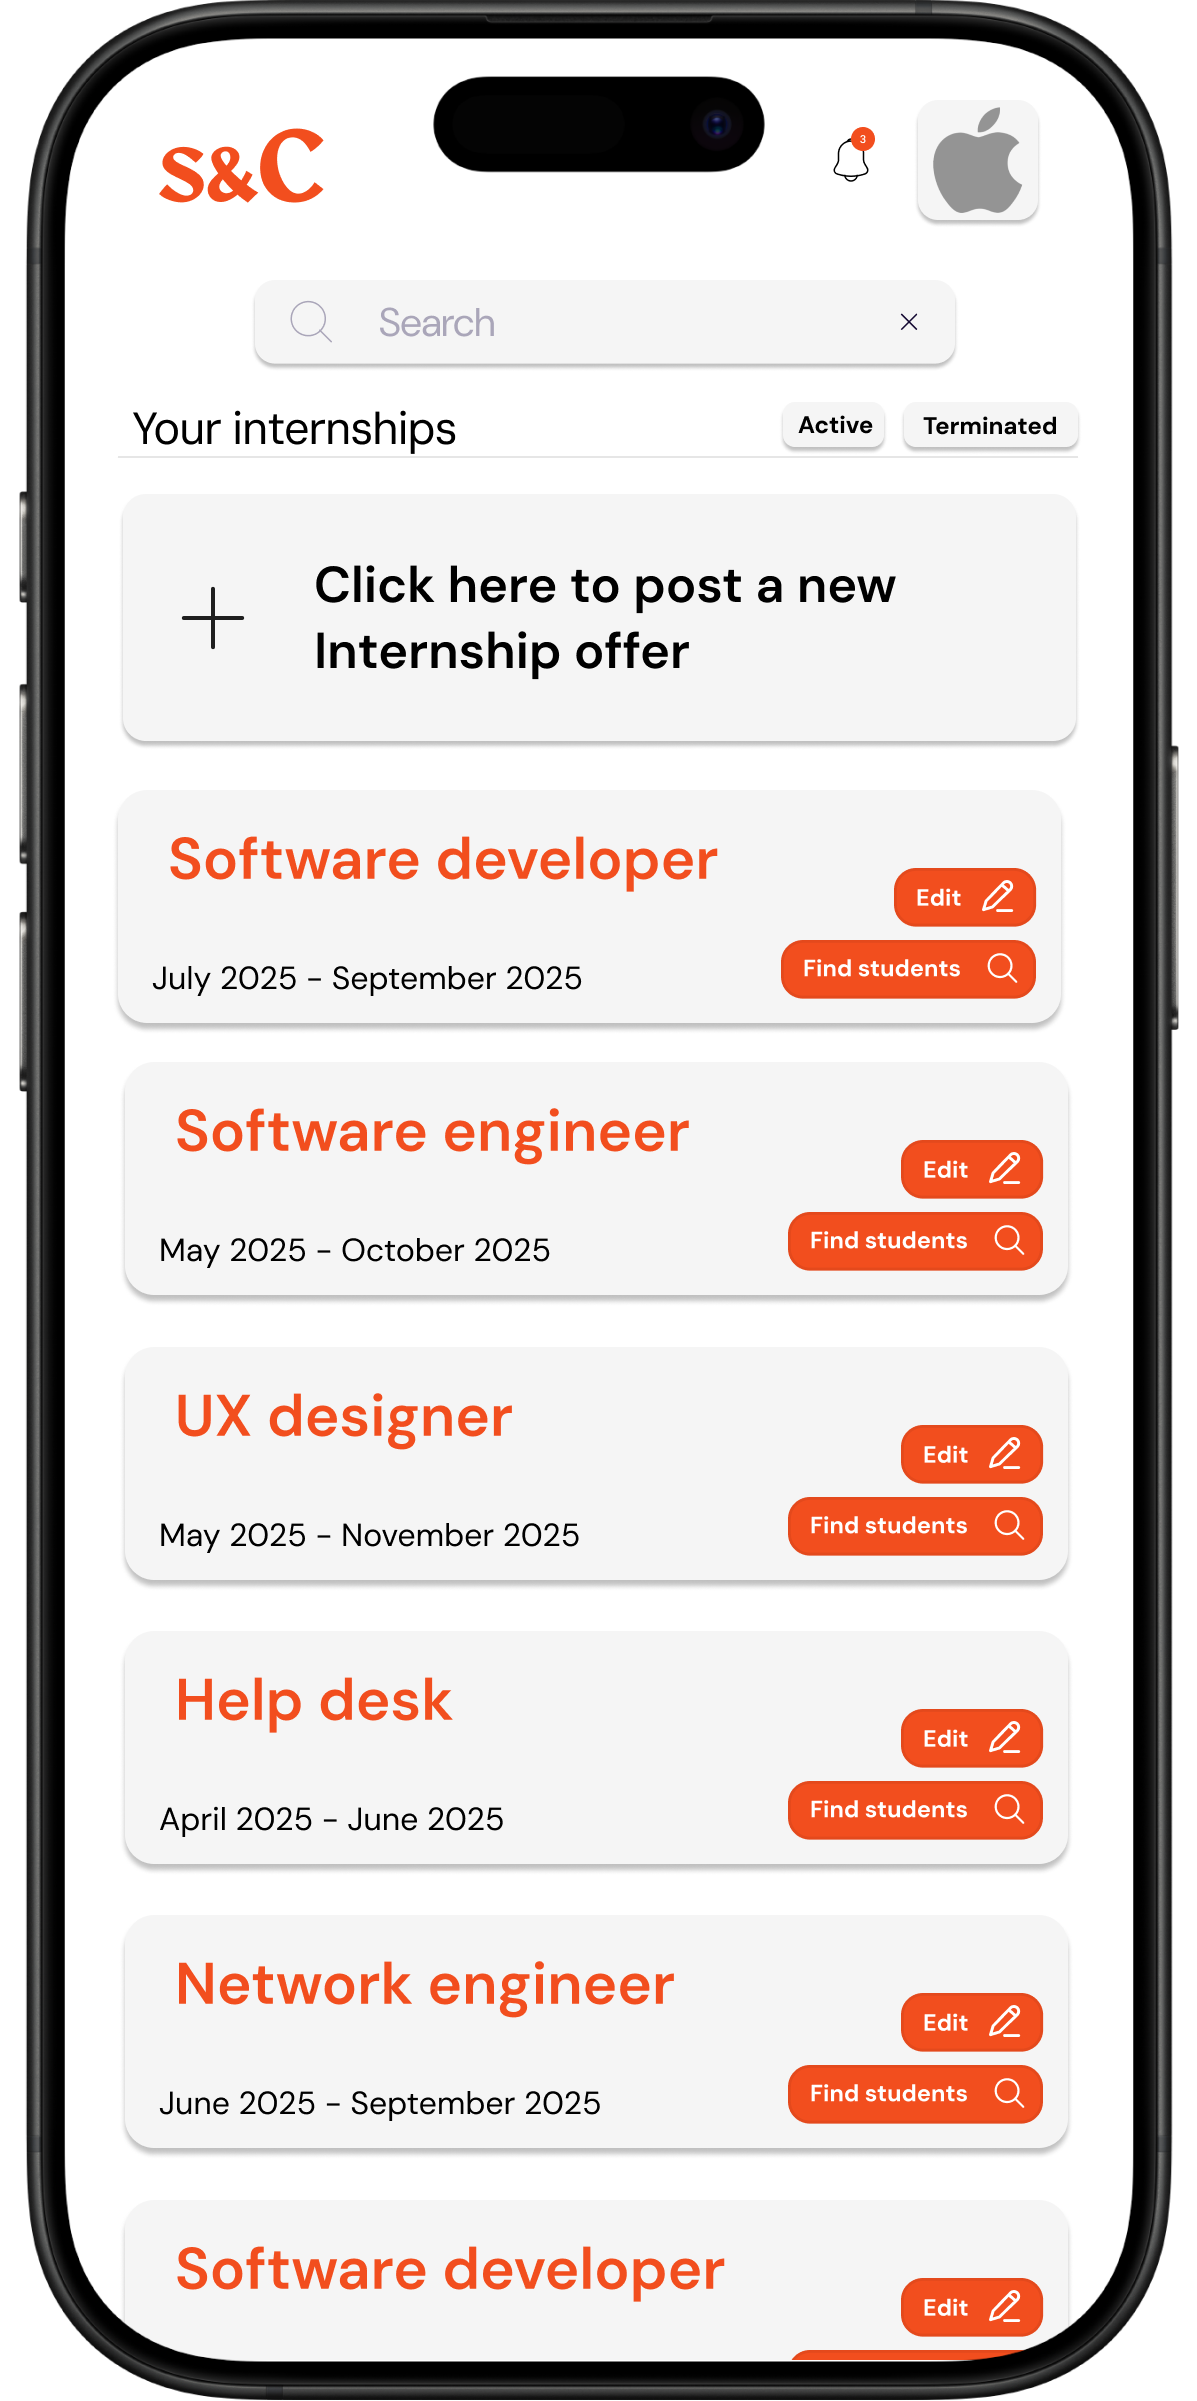
\includegraphics[width=0.2\linewidth]{Images/Mock-up/mobile homepage company.png}
    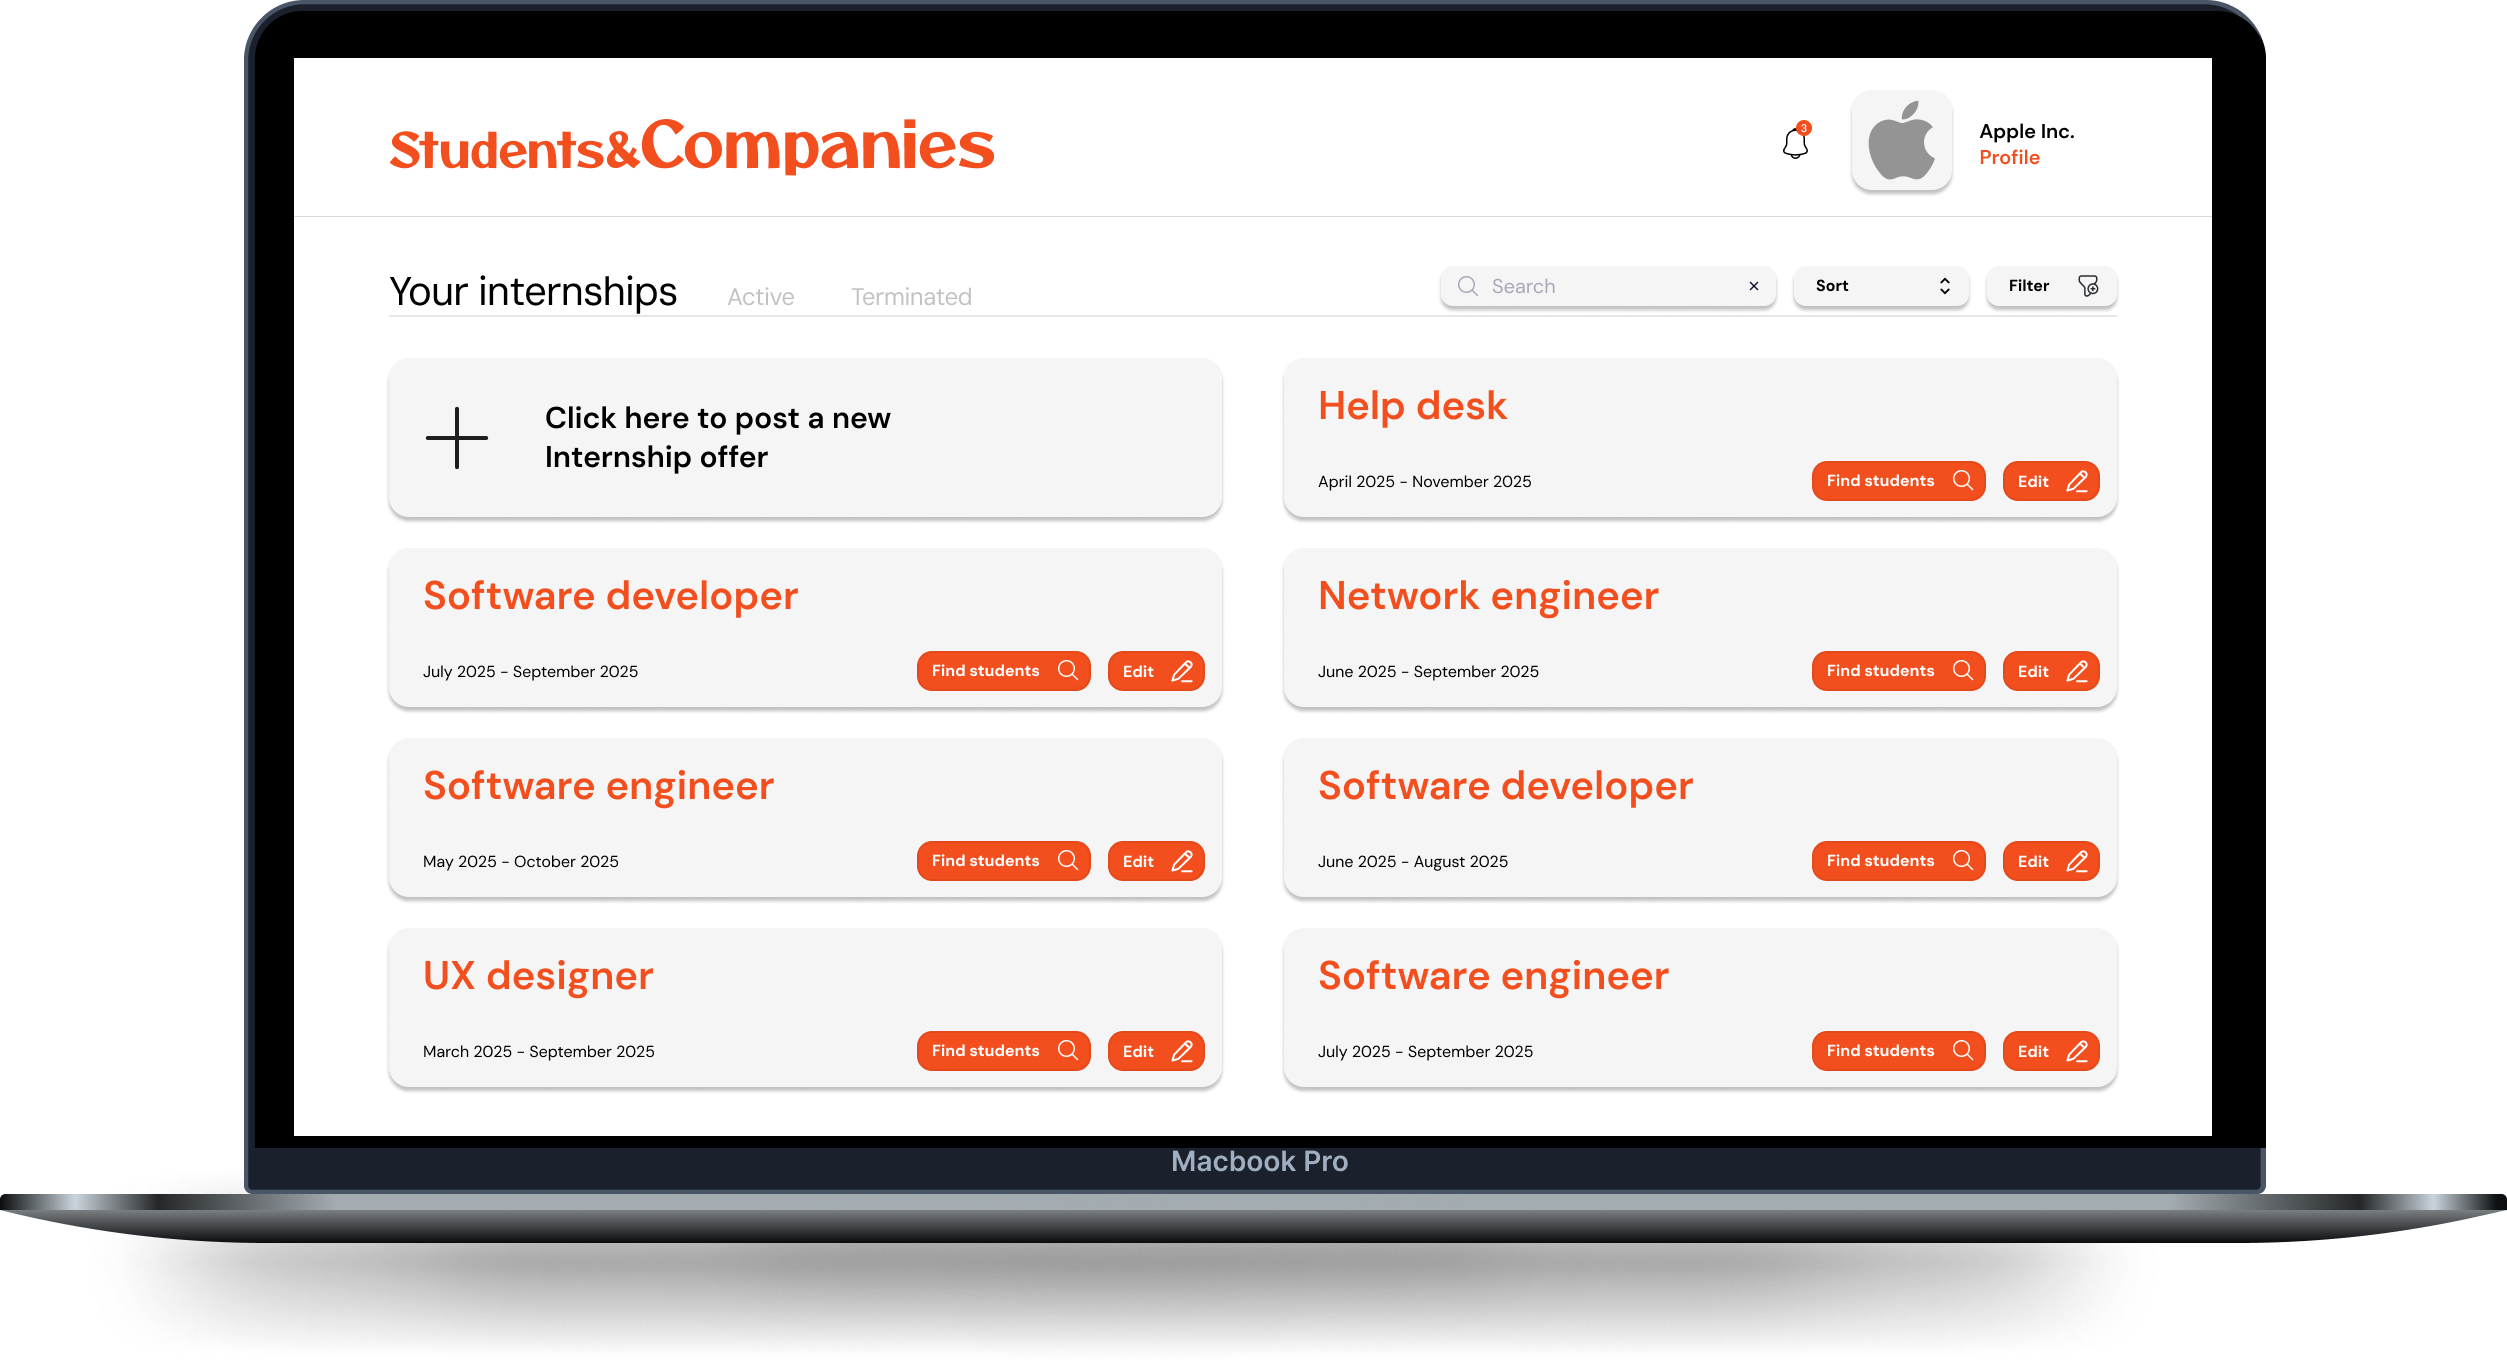
\includegraphics[width=0.75\linewidth]{Images/Mock-up/homepage company.png}
    \caption{S\&C Company Homepage Design}
    \label{fig:homepage-design}
\end{figure}

\subsection{Internship Creation and Posting Interface}

After clicking the "+" button on the homepage, the company is directed to this page where they can create a new internship post. Here, they can complete a new Internship offer post creation by filling out all the required fields in the form or return to the homepage without completing the action. \\

\begin{figure}[H]
    \centering
    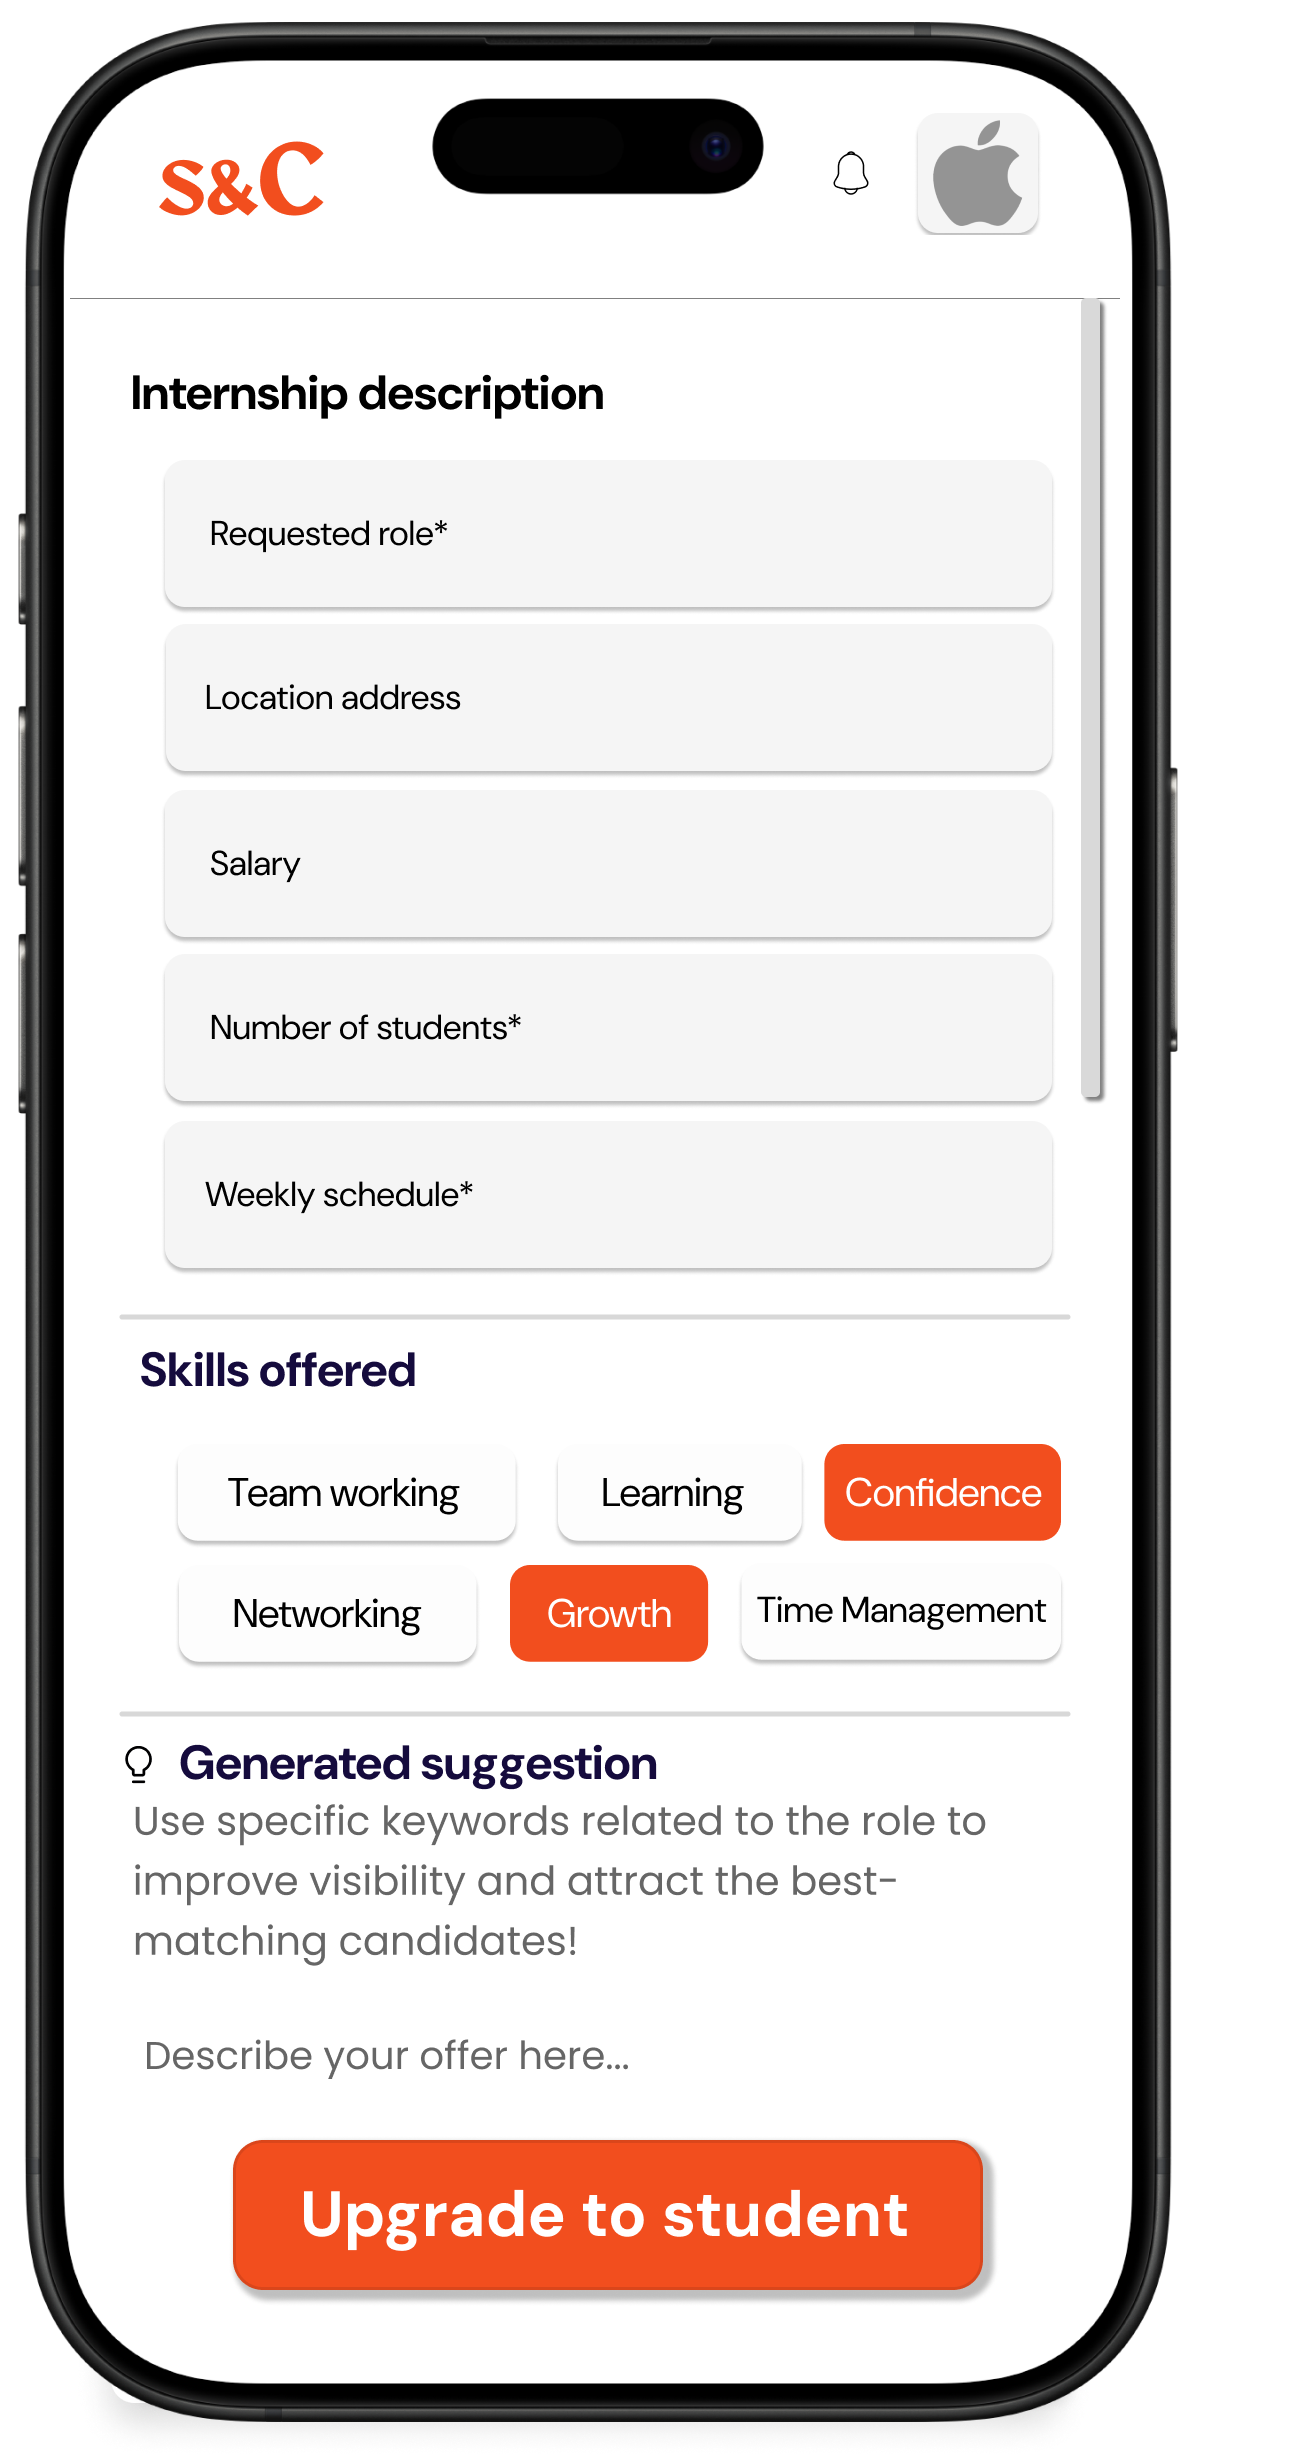
\includegraphics[width=0.2\linewidth]{Images/Mock-up/mobile post an internship.png}
    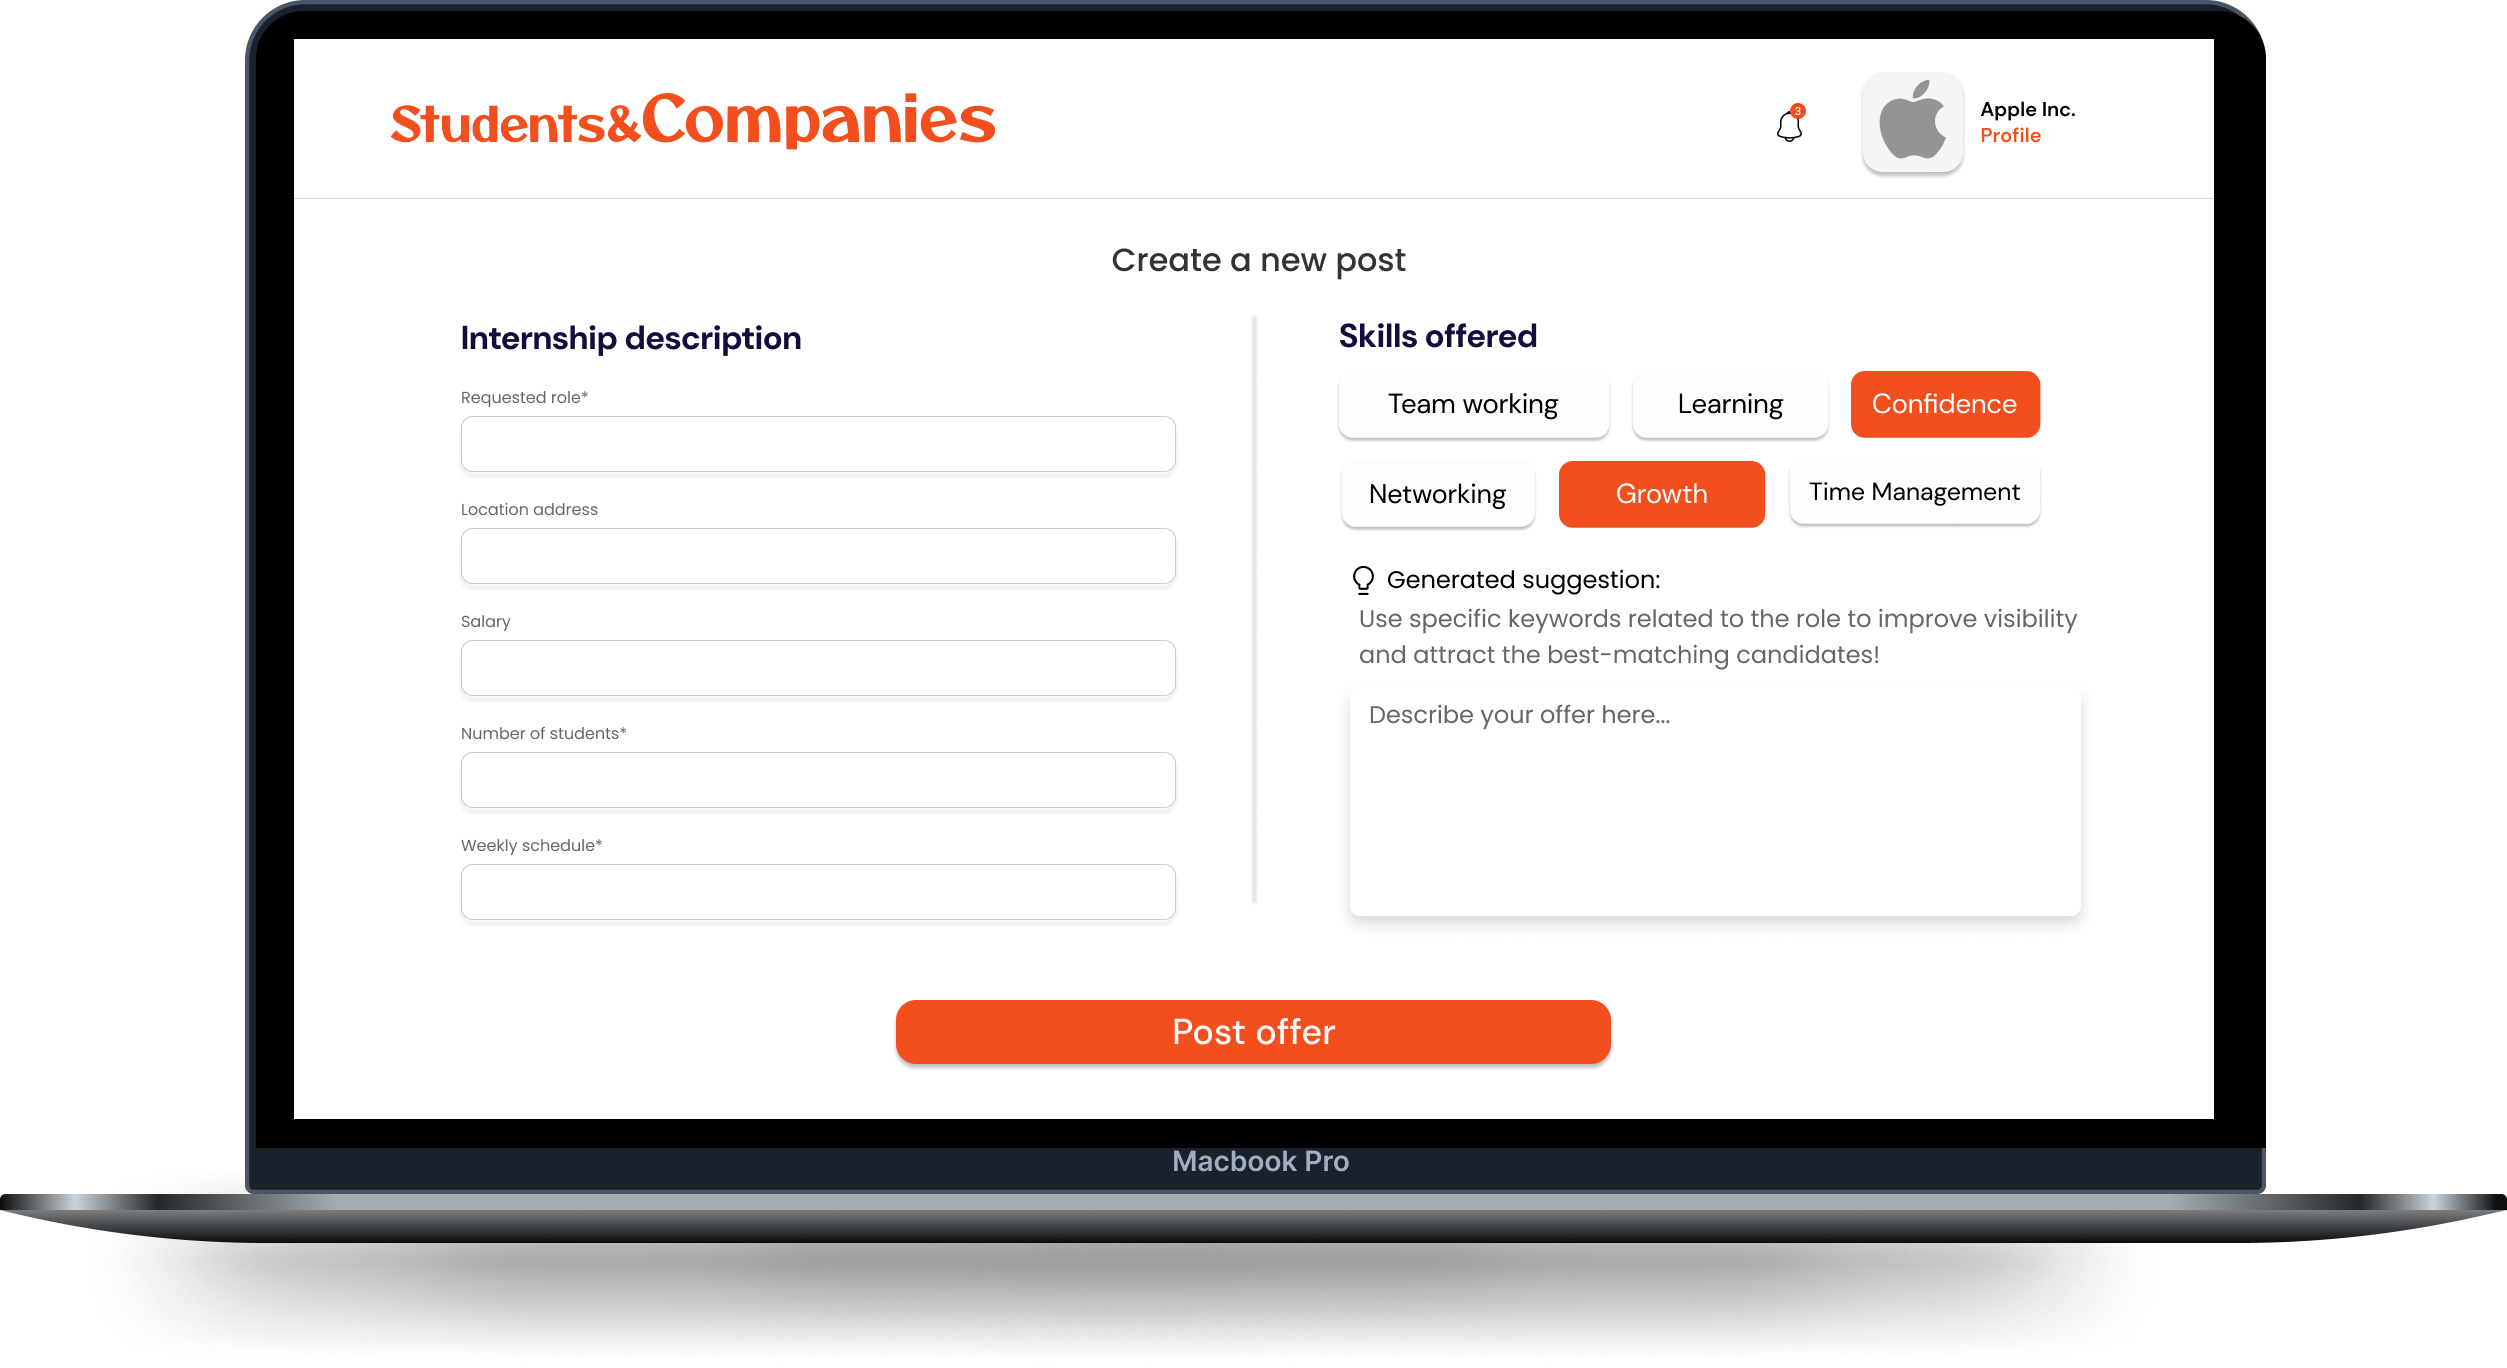
\includegraphics[width=0.75\linewidth]{Images/Mock-up/Post an internship.png}
    \caption{S\&C Company Post An Internship Page Design}
    \label{fig:homepage-design}
\end{figure}

\subsection{Applicants and Candidates Manager Interface}

After clicking the "Find students" button on the homepage, the company is directed to this page where they can find the most suitable students for their internship. The applicants are listed first, followed by others ordered by the matchmaking score. On this page they can:

\begin{itemize} 
    \item Open the student's details page by clicking the student's box. 
    \item Download directly a CV of a specific student by clicking on the "View CV" button in the student's box. 
    \item Change the listing order (e.g., by name or age) by clicking on the "sort" button. 
    \item apply filters to exclude students based on specific characteristics (e.g., role or university attended) by clicking on the "filter" button. 
    \item Search for students by name by typing it in the search bar. 
\end{itemize} \\

\begin{figure}[H]
    \centering
    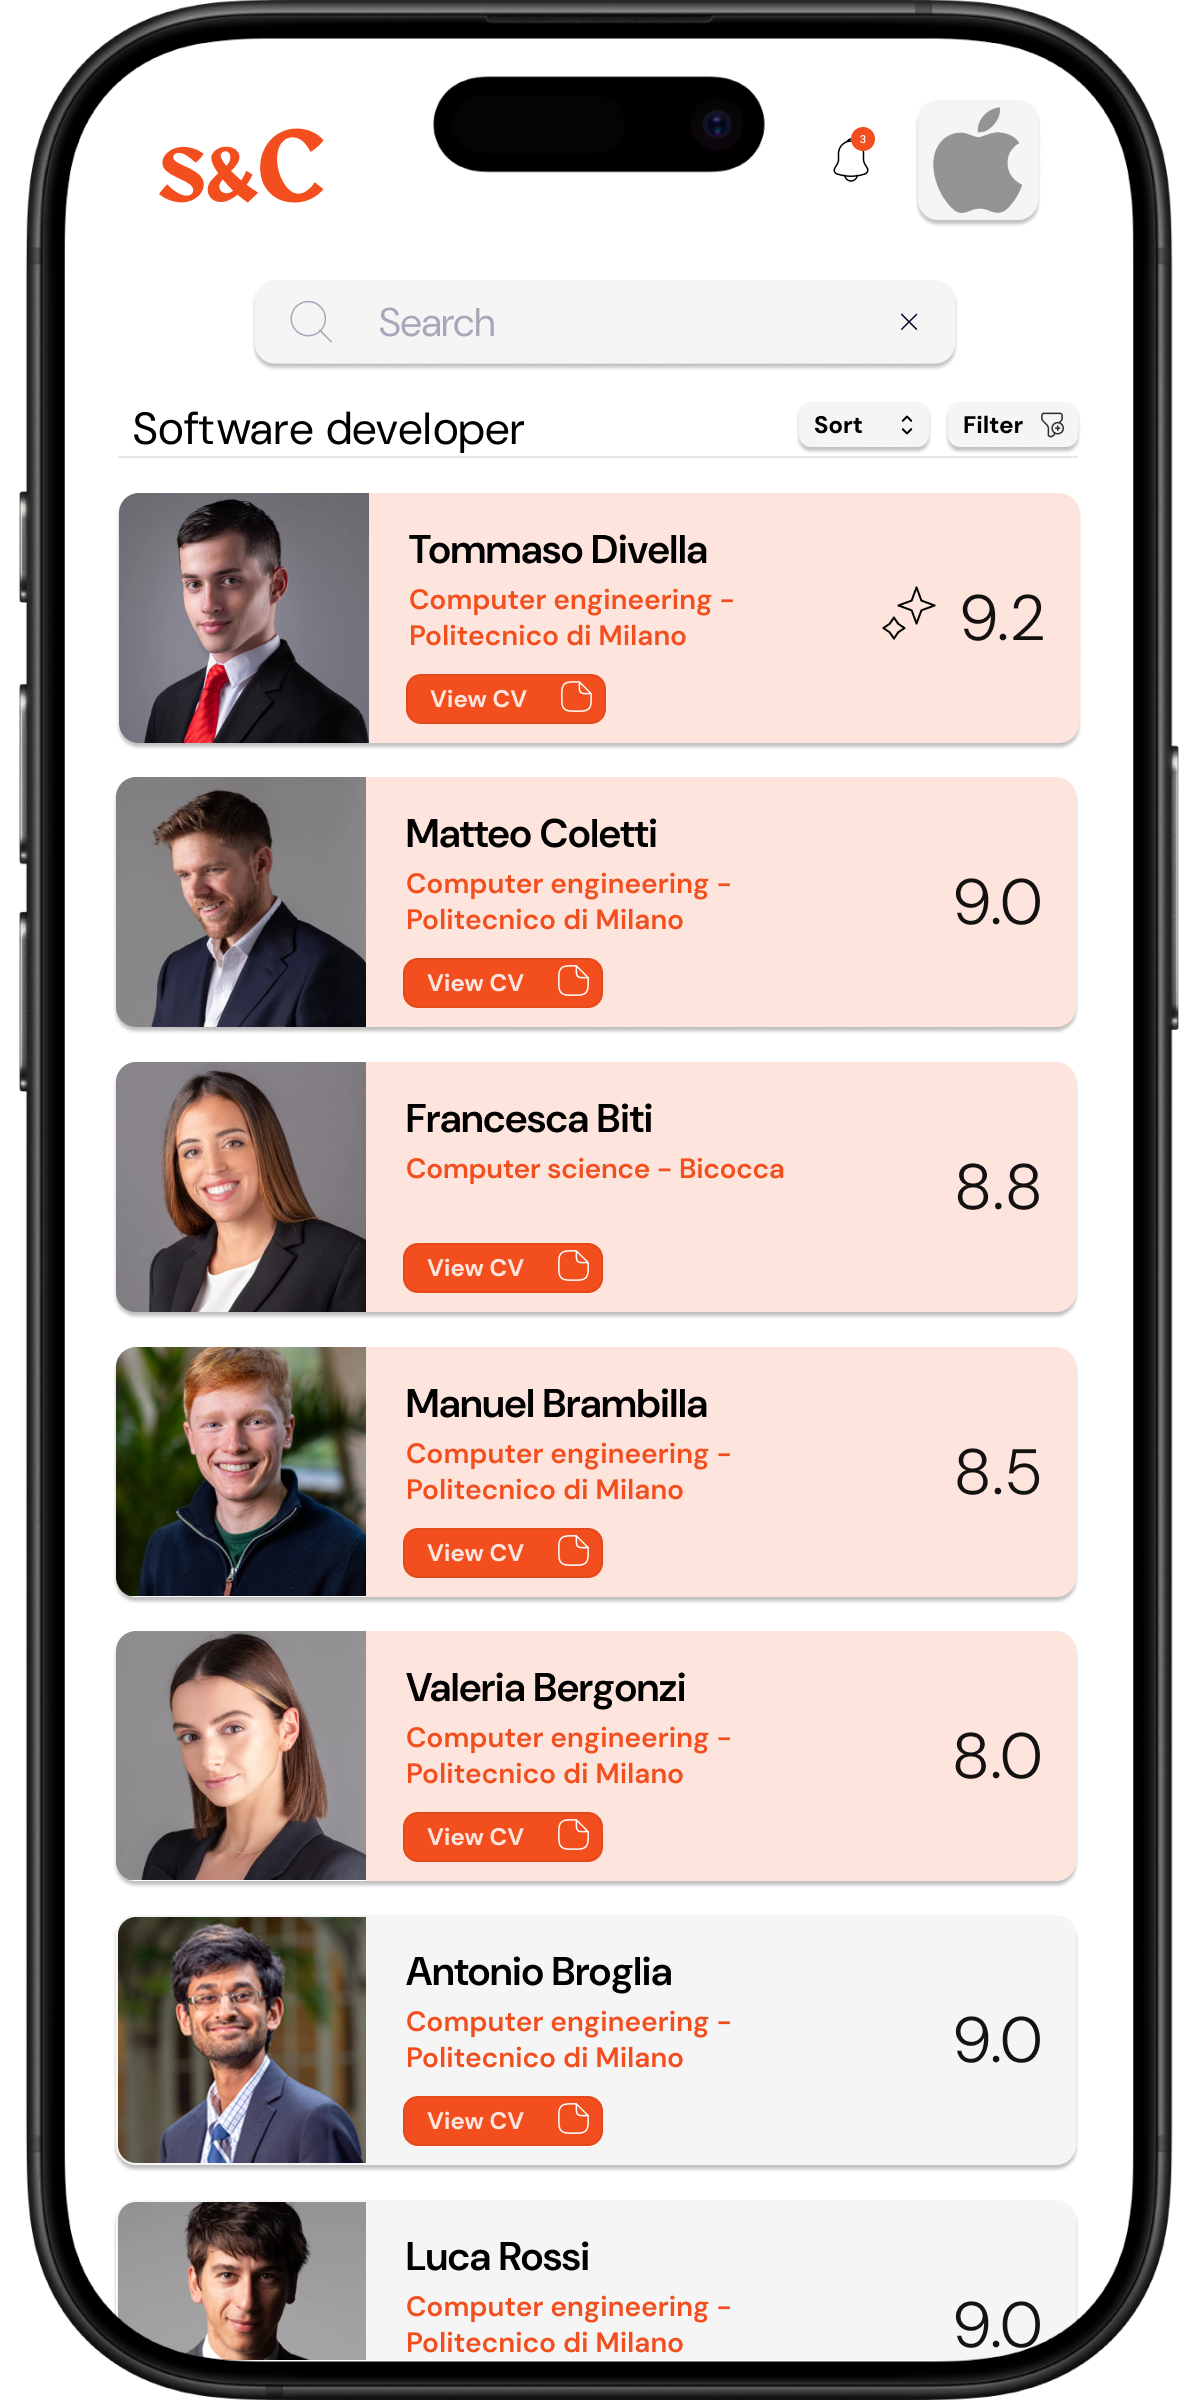
\includegraphics[width=0.2\linewidth]{Images/Mock-up/mobile candidate page company.png}
    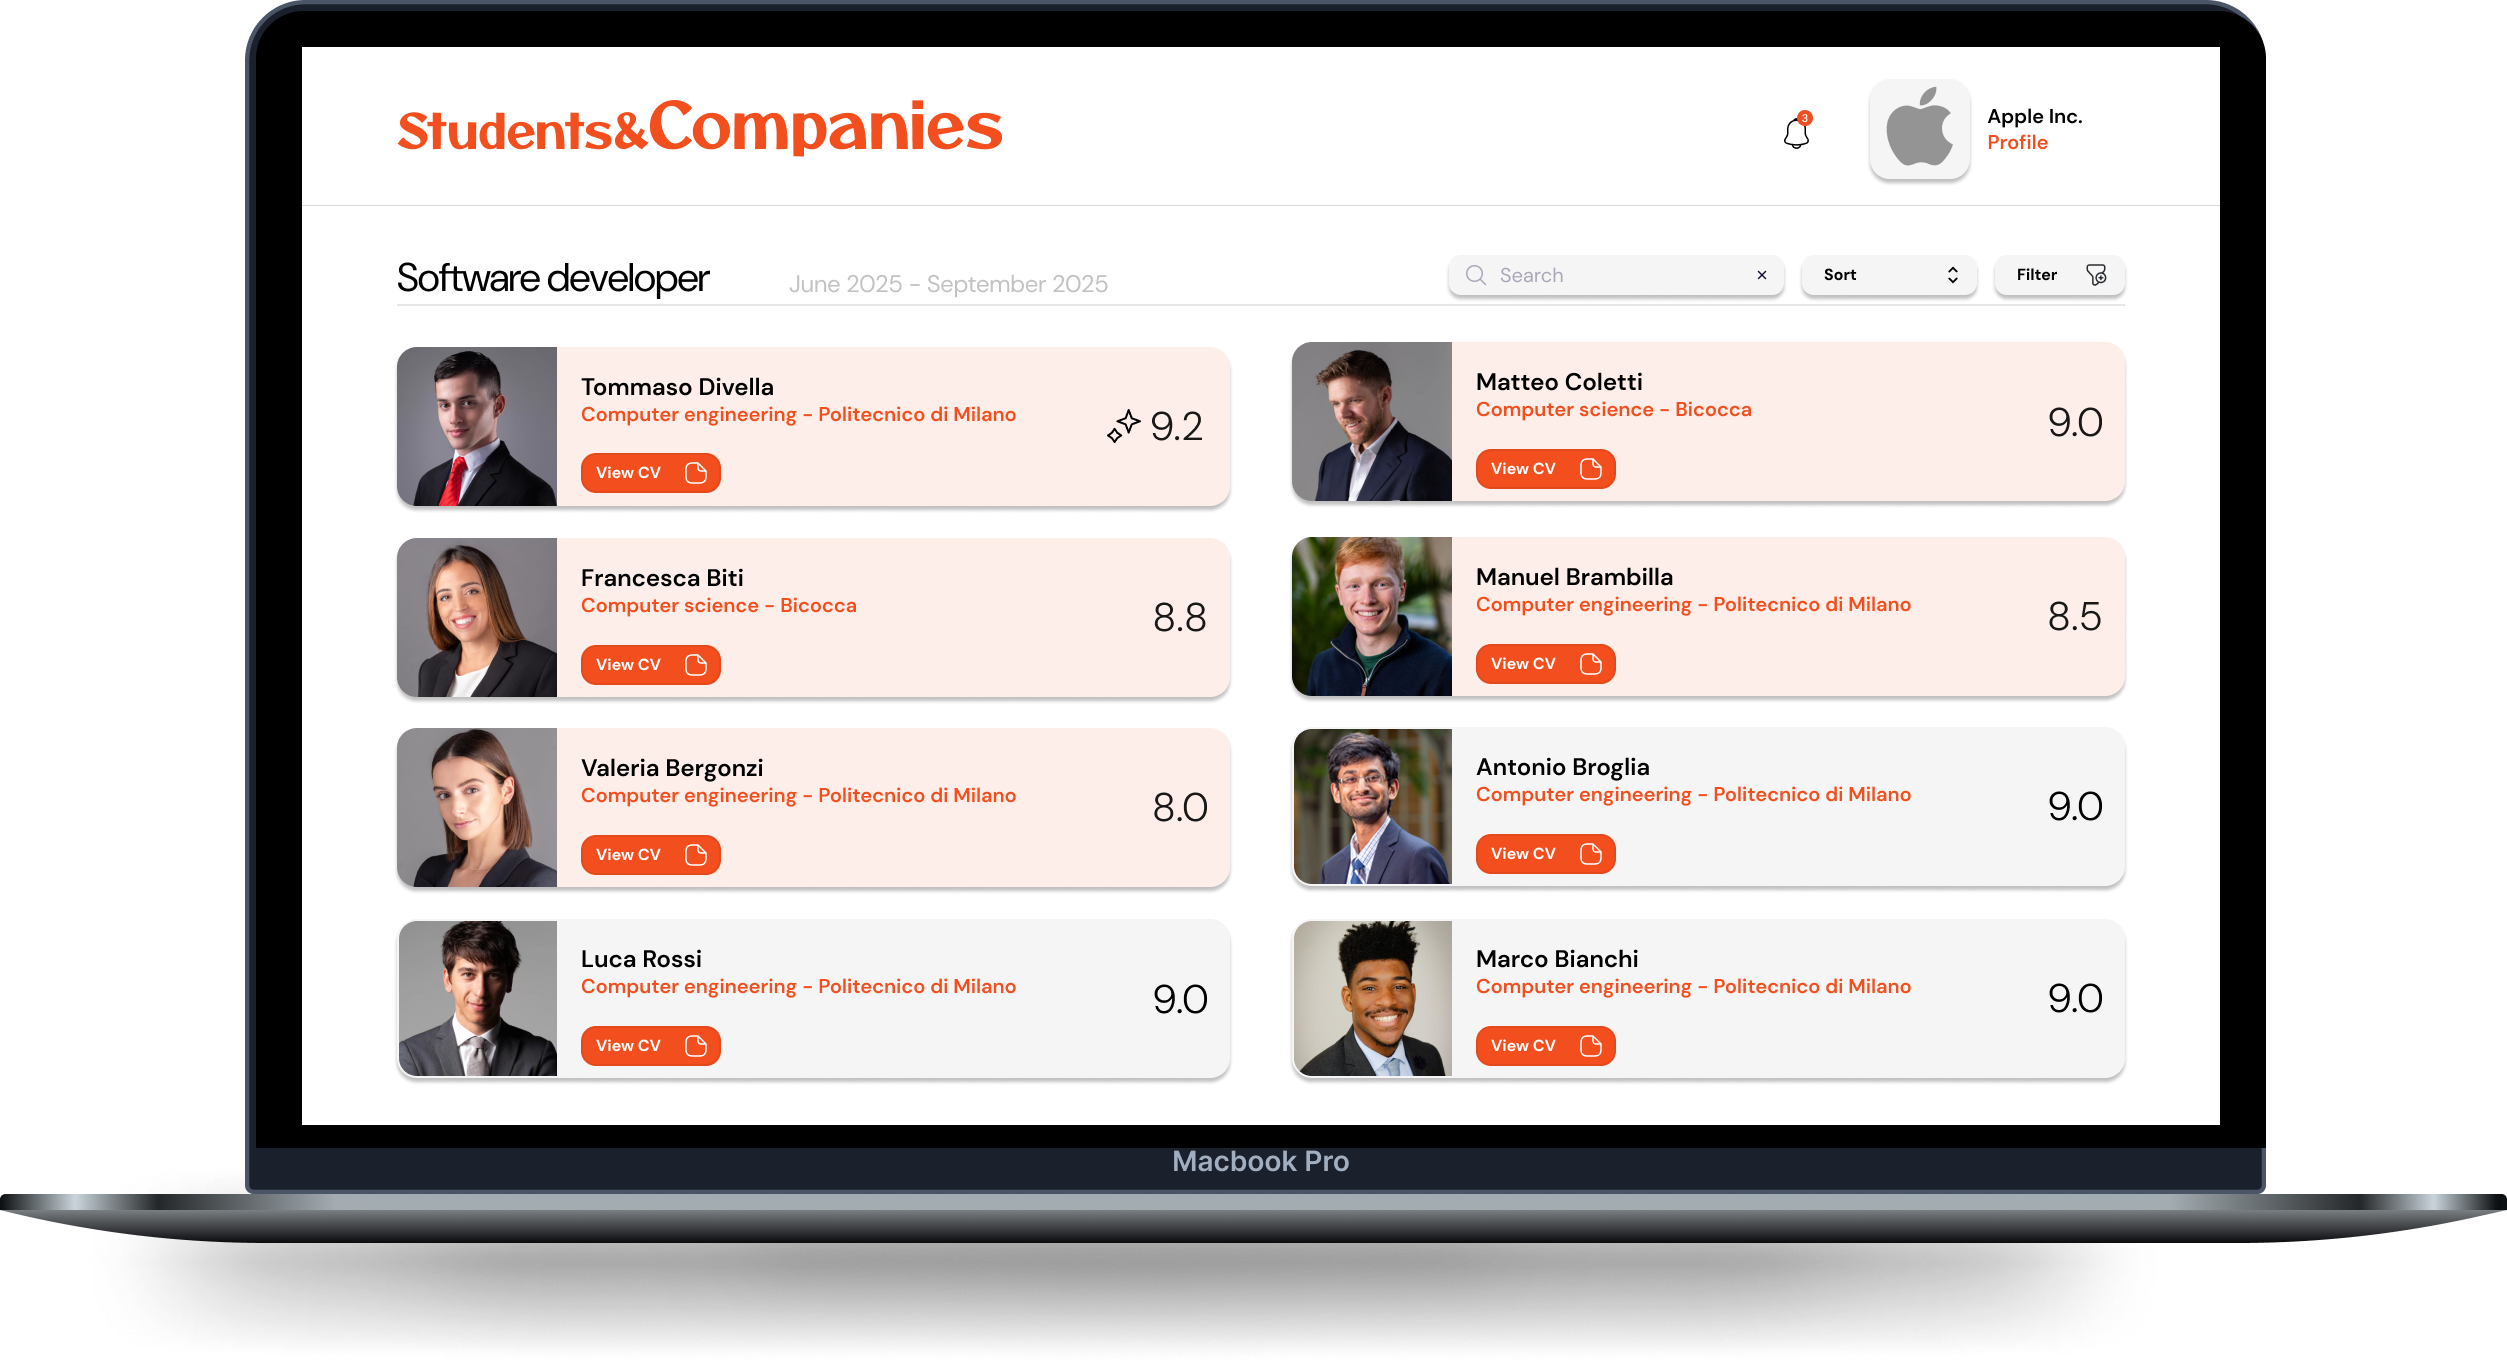
\includegraphics[width=0.75\linewidth]{Images/Mock-up/cadidates page company.png}
    \caption{S\&C Company Candidates For An Internships Page Design}
    \label{fig:homepage-design}
\end{figure}

\subsection{Applicant/Candidate Details Interface}

The company can access this page by clicking the student's box on their candidates page for an internship. On this page, they can read all the details about the candidate and, if interested, decide to open the pop-up where they can propose a meeting for an interview by clicking the respective button. The details are displayed on the right half of the page, so the company can directly view other candidates' details by clicking on another box, as their list remains open on the left half. \\

\begin{figure}[H]
    \centering
    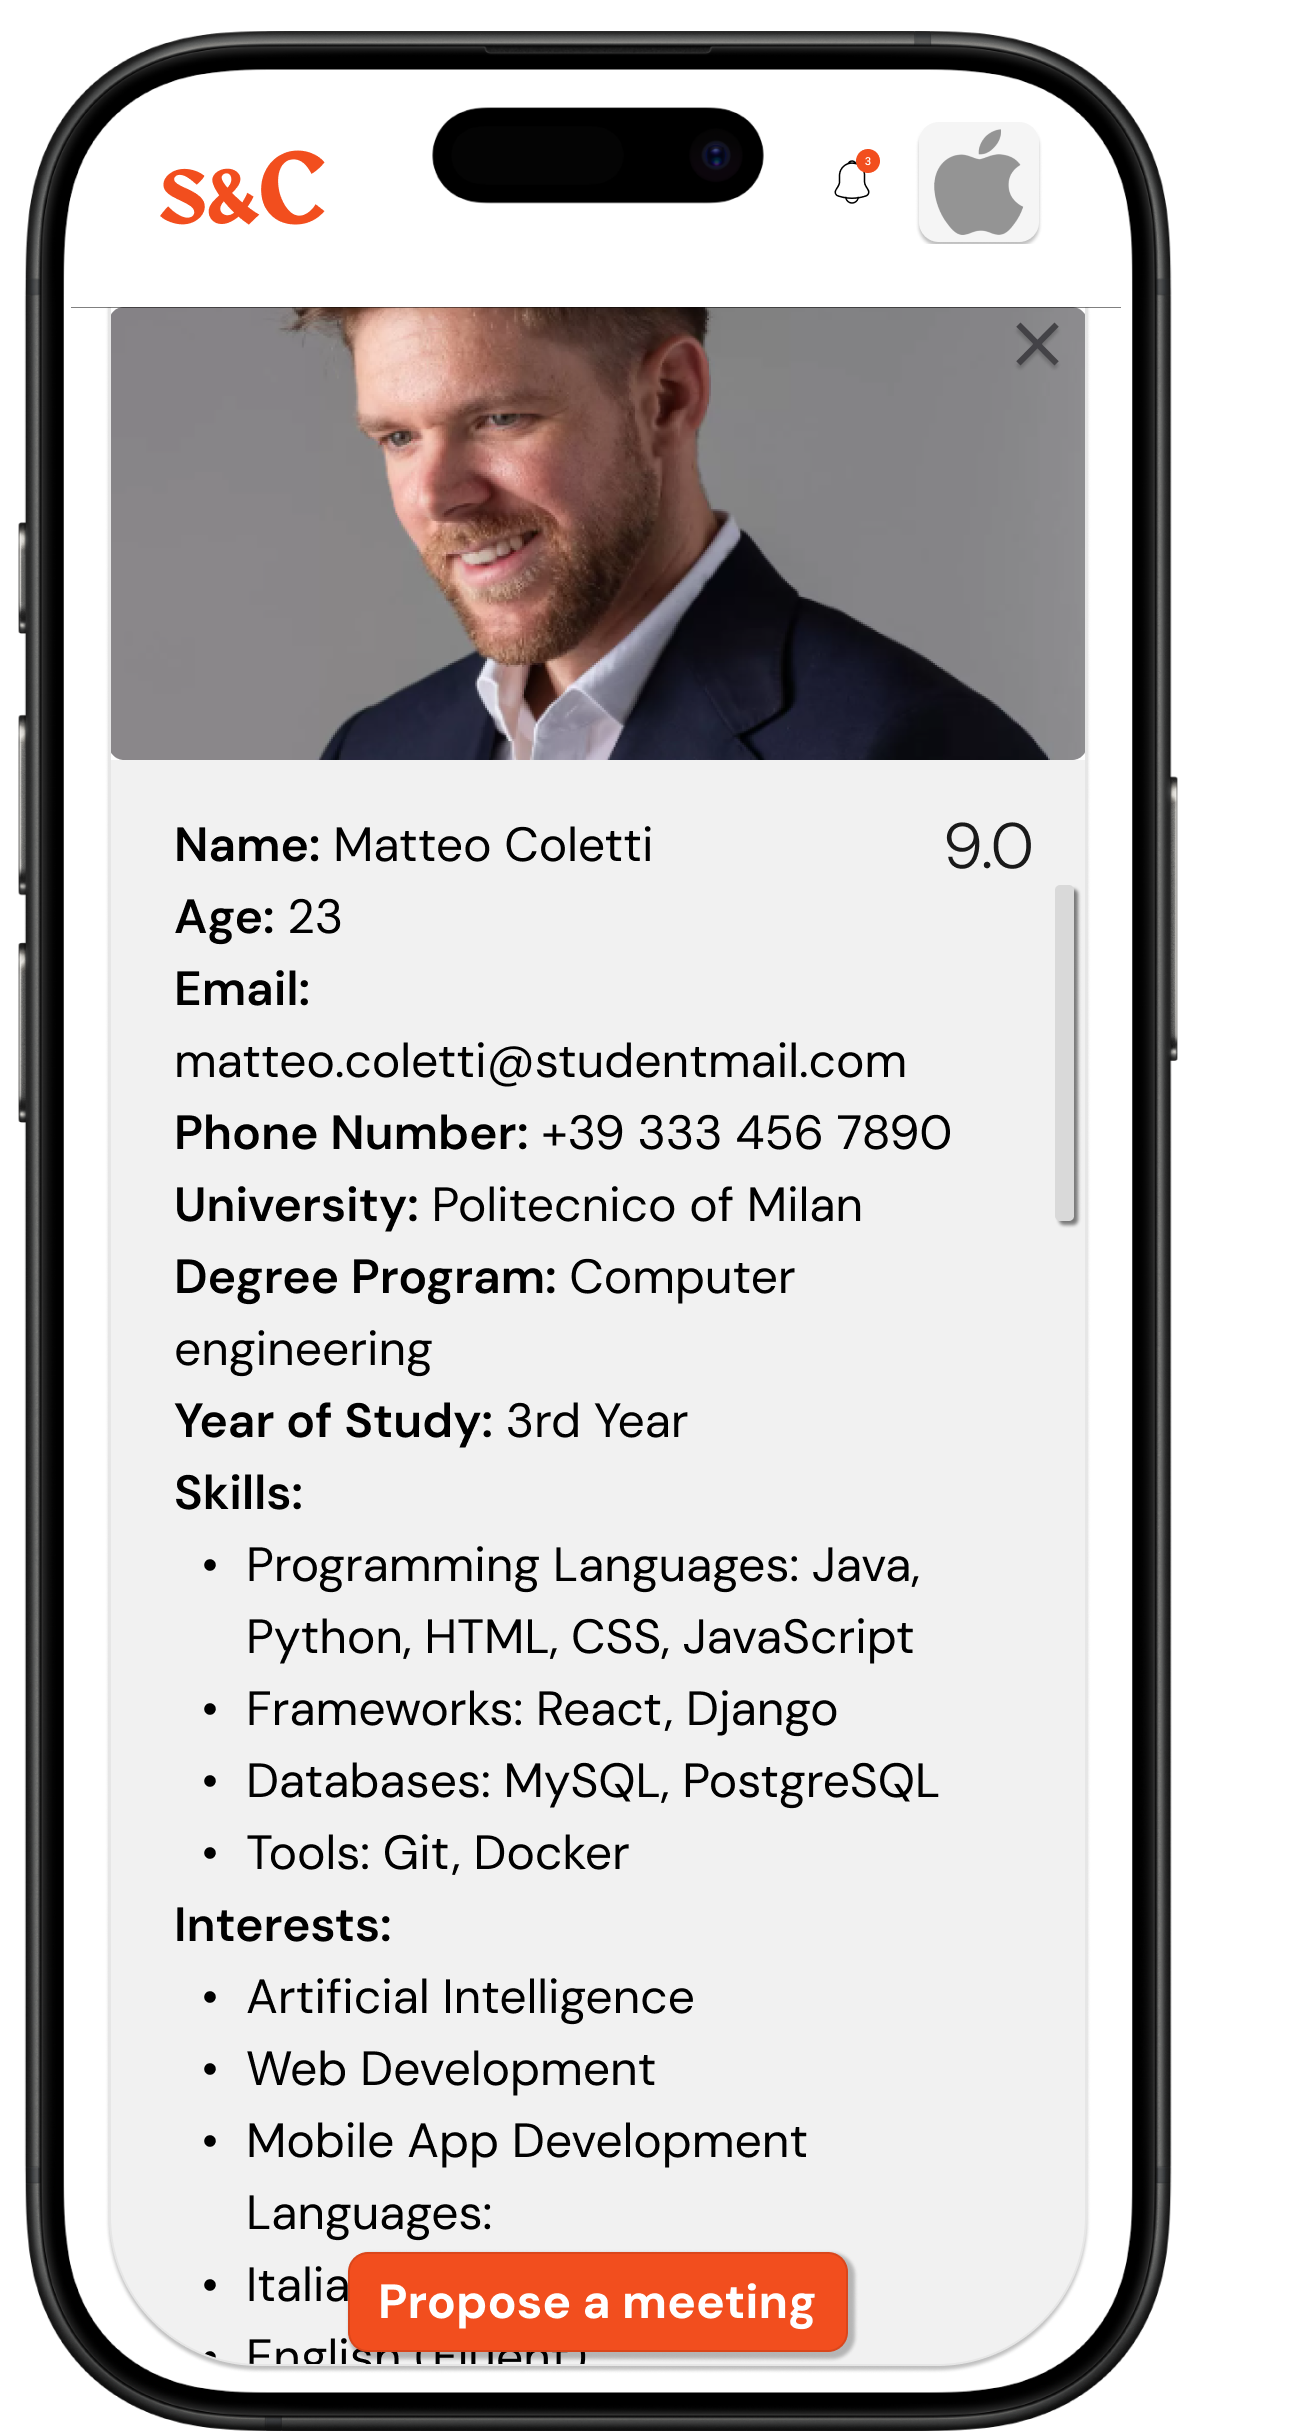
\includegraphics[width=0.2\linewidth]{Images/Mock-up/CandidateDetailsMobile.png}
    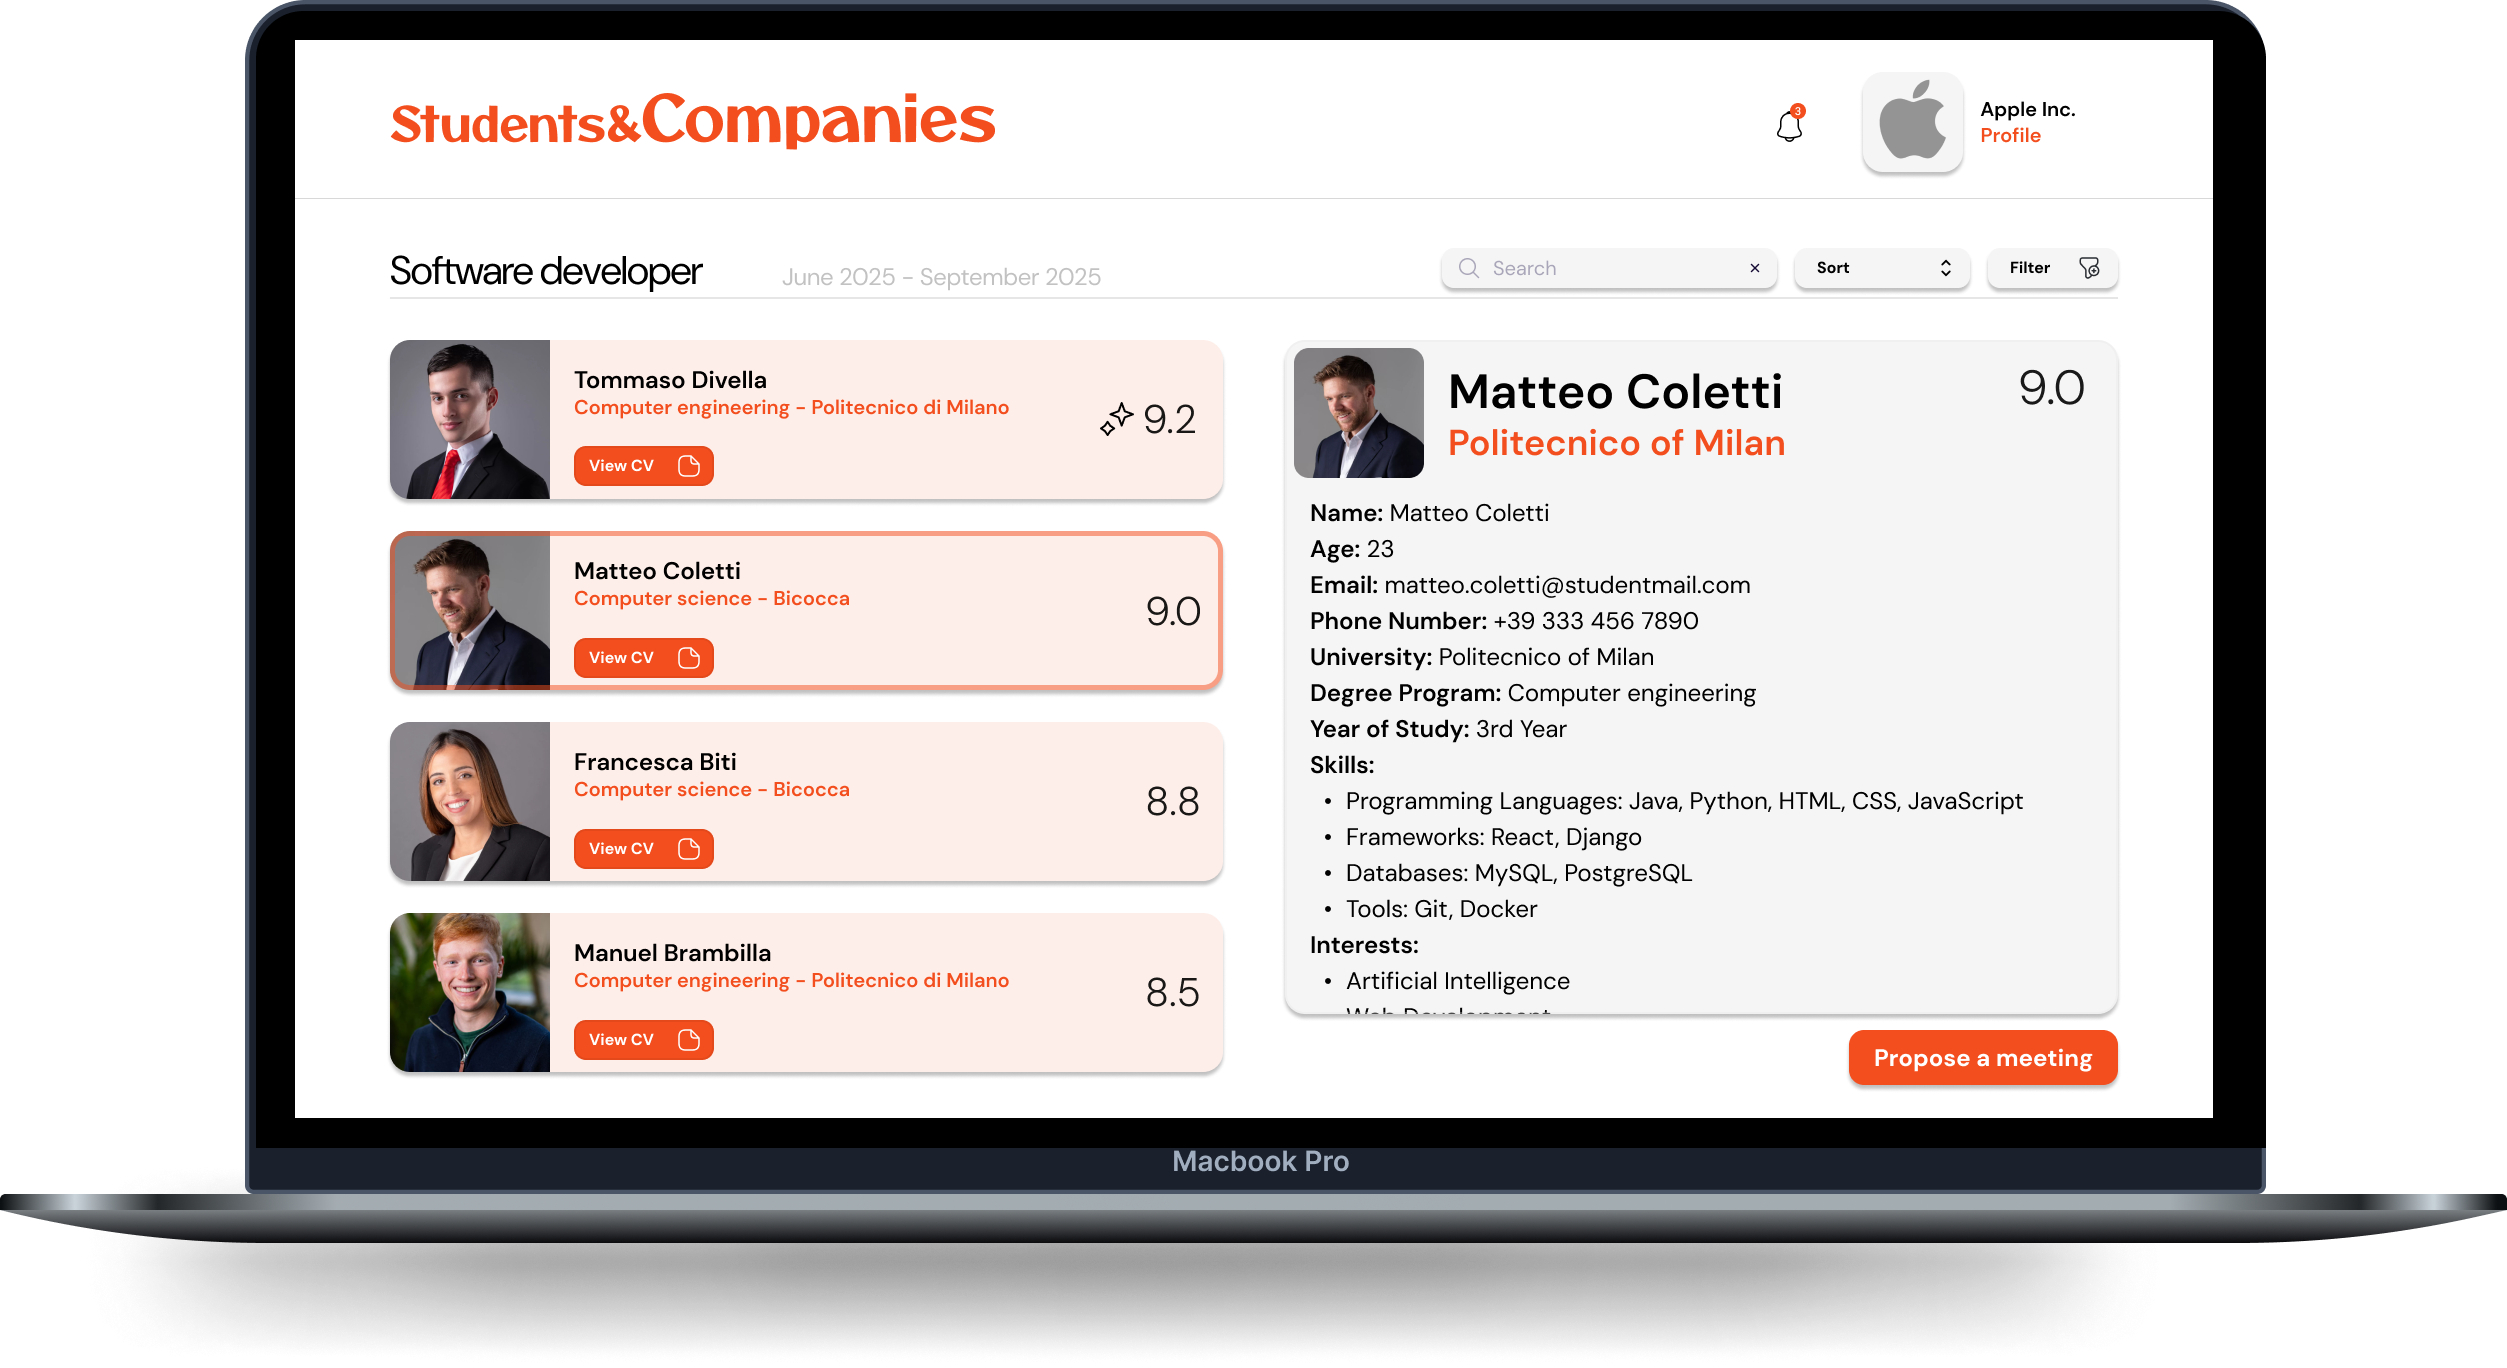
\includegraphics[width=0.75\linewidth]{Images/Mock-up/CandidateDetailsPC.png}
    \caption{S\&C Company Candidate details Page Design}
    \label{fig:homepage-design}
\end{figure}

\subsection{Propose a Meeting Interface}

This pop-up is shown to the company after they click on the "Propose a meeting" button. Here, they can select a day to schedule a meeting for the selected candidate by clicking on a day in the calendar and entering a start time and end time. The already occupied days are displayed. Before submitting the proposal, the company must write a message for the candidate. This action will send a notification to the student, who can then choose whether to accept it or not. After clicking the "Send schedule" button, the company is brought back to their homepage. \\

\begin{figure}[H]
    \centering
    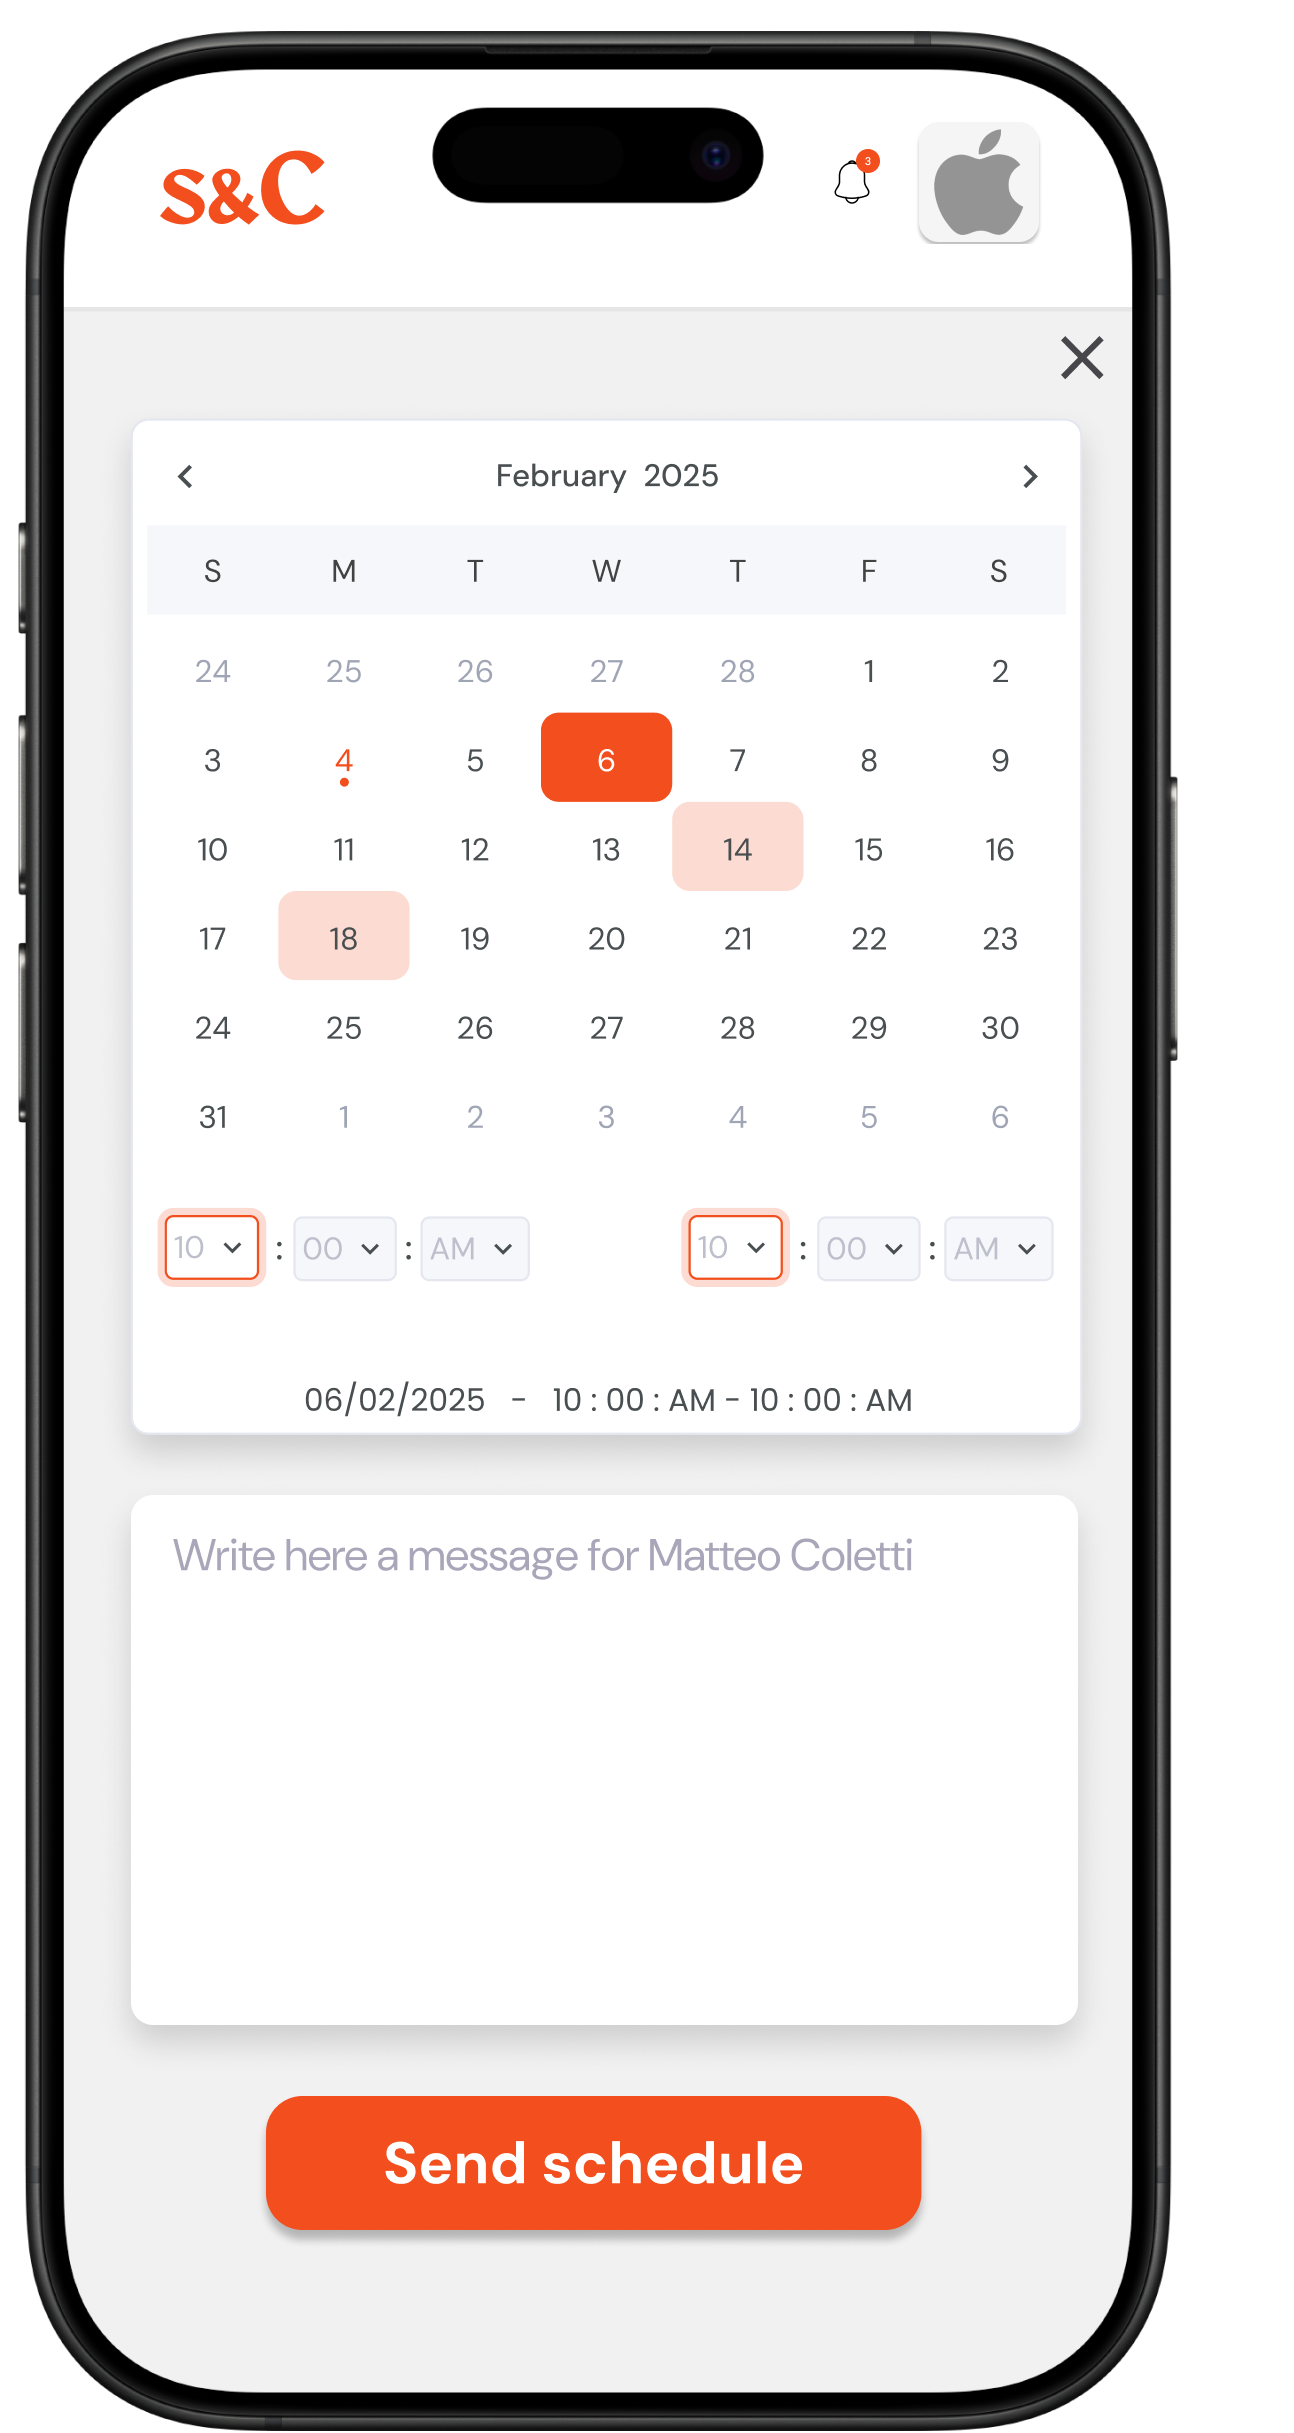
\includegraphics[width=0.2\linewidth]{Images/Mock-up/InterviewProposalMobile.png}
    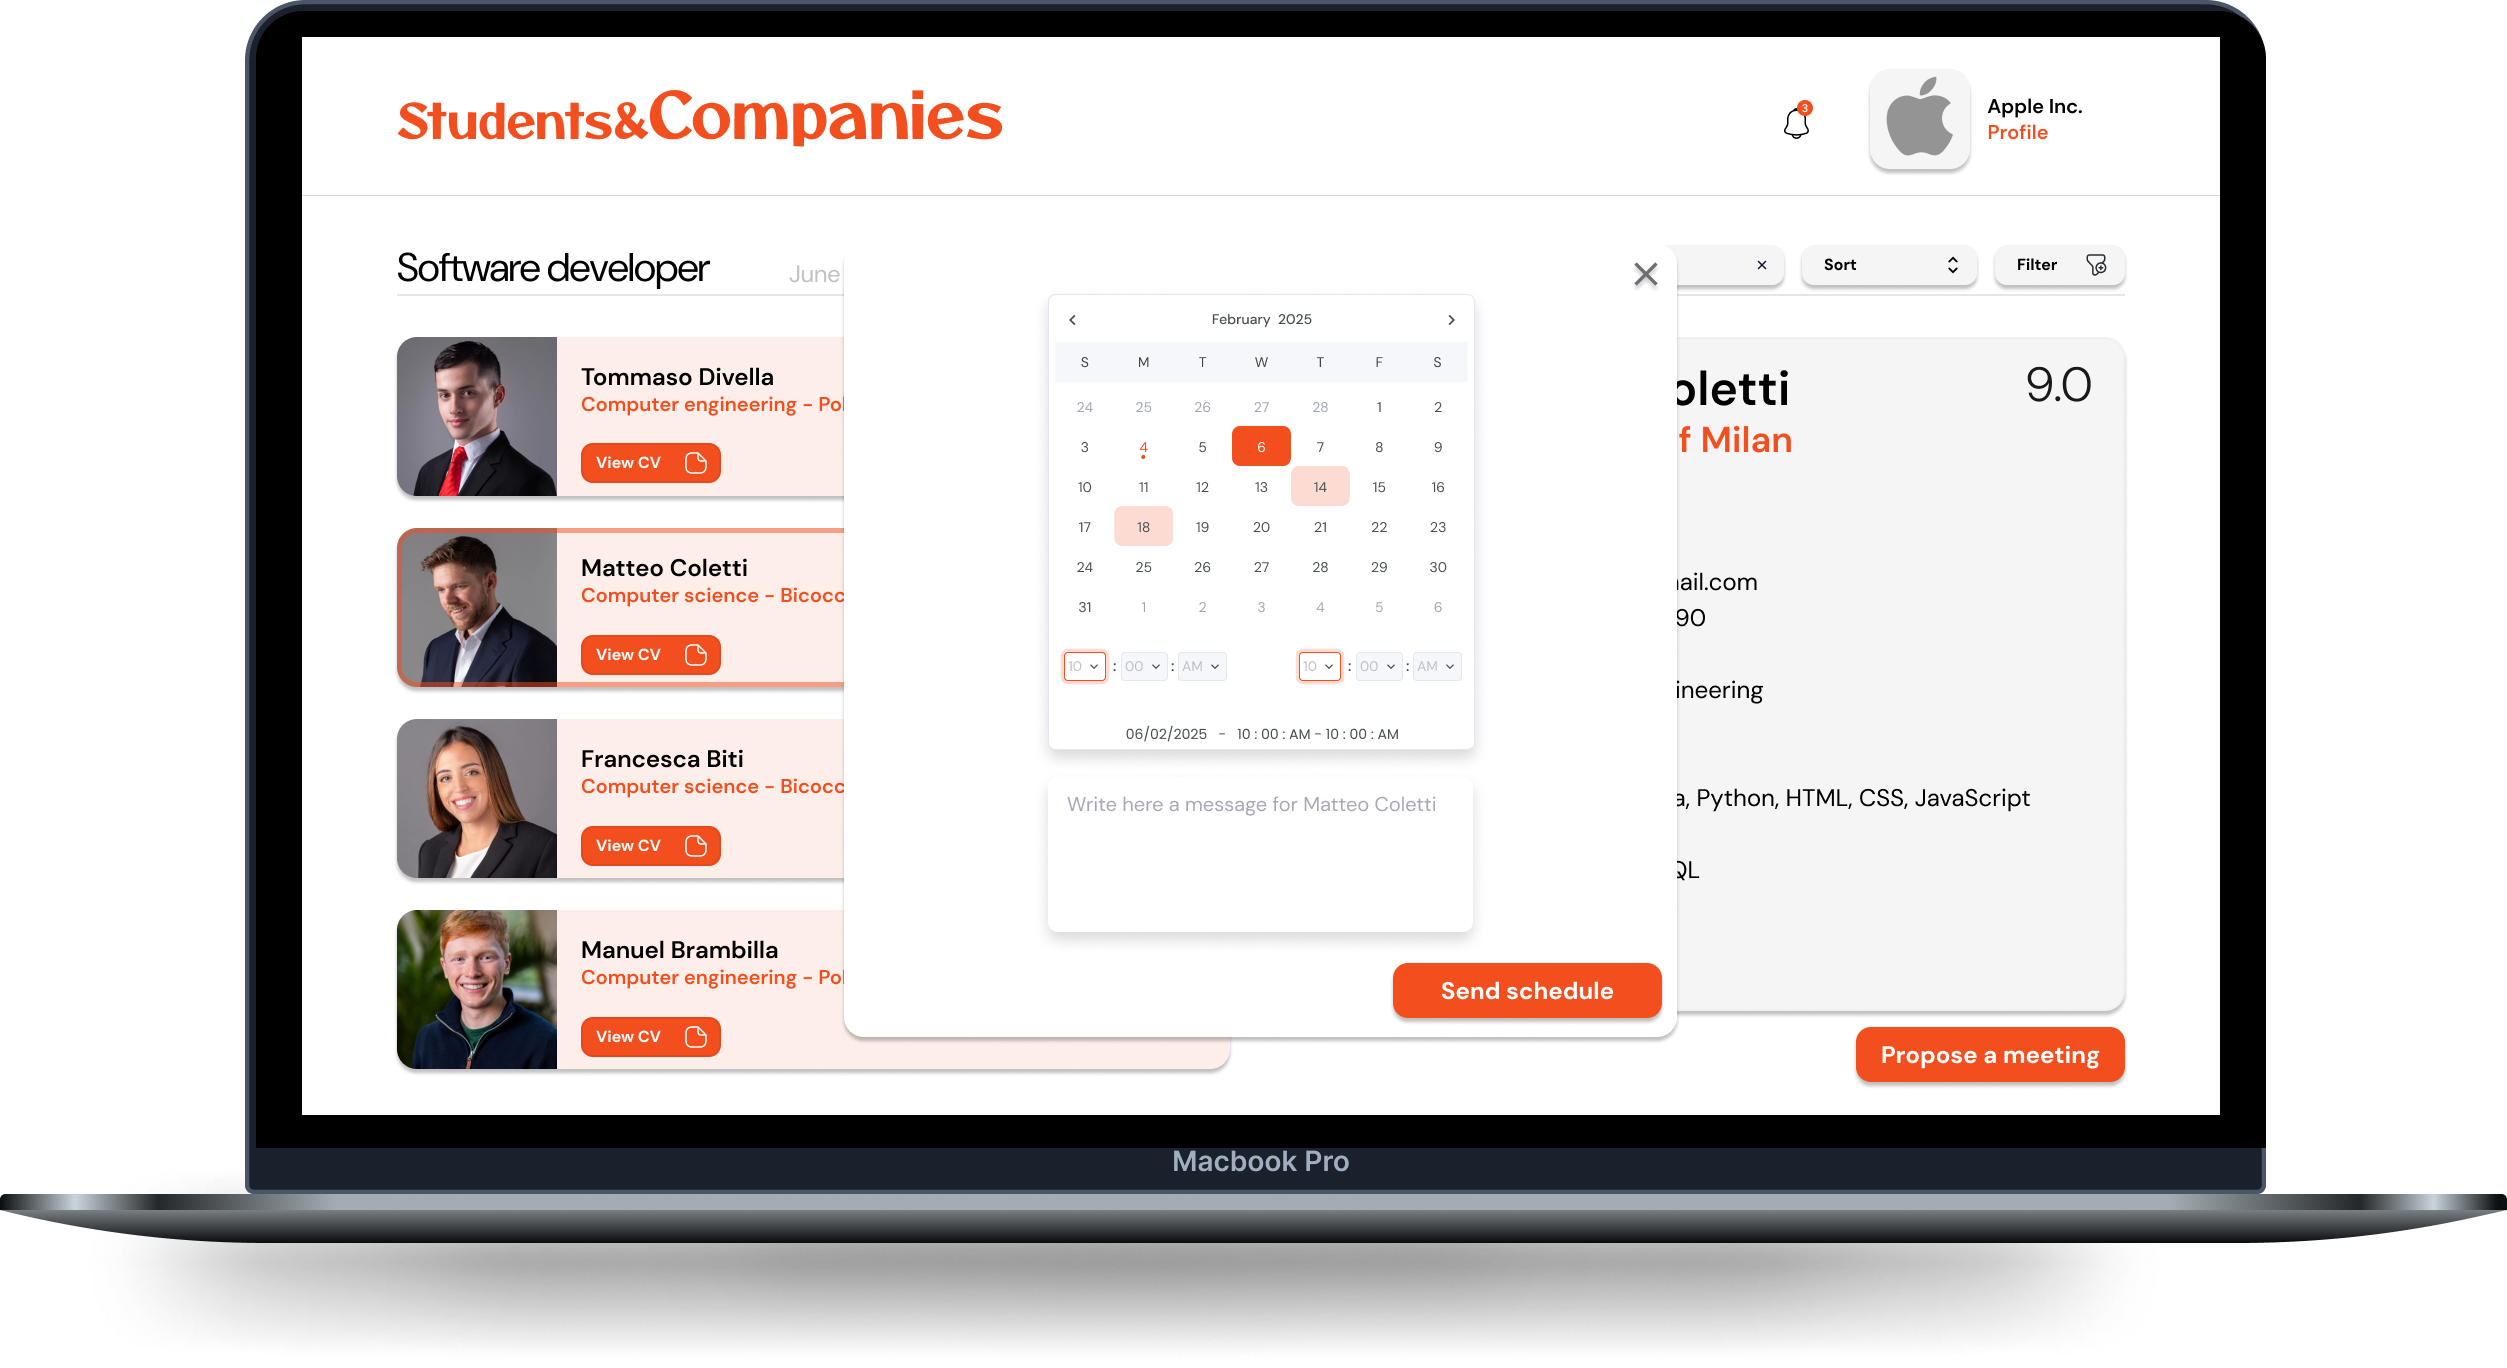
\includegraphics[width=0.75\linewidth]{Images/Mock-up/InterviewProposalPC.png}
    \caption{S\&C Company Propose A Meeting Page Design}
    \label{fig:homepage-design}
\end{figure}

\section{University Interface}

Universities can access this page after logging in with the provided credentials. On this page, they can browse all current internships for their students and see if there are complaints on them. The click of the notification button displays all the complaint notifications and the click of the "Review complaint" button opens the complaint handling page. \\

\begin{figure}[H]
    \centering
    \includegraphics[width=0.9\linewidth]{Images/Mock-up/University homepage.png}
    \caption{S\&C University Homepage Design}
    \label{fig:homepage-design}
\end{figure}

\subsubsection{Complaint Manager Interface}
The complaint handling page is opened on half page. The university, after reasoning about the new complaint from student or company, can decide if it's enough relevant to interrupt the internship or not, "resolving" it. These actions can be done by clicking on the designated button. After doing one of these, the university goes back to the homepage. \\

\begin{figure}[H]
    \centering
    \includegraphics[width=0.9\linewidth]{Images/Mock-up/University complaint handle.png}
    \caption{S\&C University Complaint Handling Page Design}
    \label{fig:homepage-design}
\end{figure}


    \chapter{Requirements Traceability}
    \label{ch:requirements_traceability}%
    This chapter shows how the functional and non-functional requirements of the S\&C system described in the RASD are met. In section 4.1 we describe the mapping between the requirements found and commented in section 3.2.1 of the document RASD with the components identified in section 2.2 of this document. 

\begin{center} 
    \renewcommand{\arraystretch}{1.2} 
    \begin{longtable}{| l |p{0.7\linewidth} |} 
        \hline 
        Registration Manager 
        & [R1] S\&C system allows unregistered users to sign-up. \\ 
        & [R2] S\&C system allows registered users to verify their email address. \\ \hline 
        Login Manager 
        & [R3] S\&C system allows registered users to login.\\ \hline
        Profile Manager 
        & [R4] S\&C system allows registered users to edit their account details. \\ 
        & [R5] S\&C system allows registered users to delete their account.\\
        & [R7] S\&C system allows registered users to upgrade to a Student account or a
        Company account. \\
        & [R8] S\&C system allows registered users to verify their current academic status by validating their institutional email address.\\ \hline 
        Notification Manager 
        &[R8] S\&C system allows registered users to verify their current academic status by validating their institutional email address.\\
        & [R9] S\&C system allows registered users to update their notifications preferences.\\
        & [R15] S\&C system allows Students to receive notification when a new internship matching their profile is posted.\\
        & [R19] S\&C system allows Students to monitor the status of an application.\\
        & [R21] S\&C system allows Students to confirm their participation of a scheduled interview via a notification interface.\\
        & [R22] S\&C system allows Students to decline an interview offer via a notification interface.\\
        & [R23] S\&C system sends automated reminders to Students for upcoming interview deadlines.\\
        & [R26] S\&C system allows Students to submit feedback after completing an internship.\\
        & [R28] S\&C system allows Companies to edit an internship’s post.\\
        & [R33] S\&C system allows Companies to receive notification when a new students with an high matching score has applied.\\
        & [R36] S\&C system allows Companies compare the answers from all candidates to facilitate the selection process.\\ 
        & [R44] S\&C system allows universities to collect complaints raised by Companies.\\
        \hline 
        Matchmaking Manager 
        & [R6] S\&C system allows registered users to view posted internships on the platform.\\ 
        & [R11] S\&C system allows Students to explore available internships.\\
        & [R12] S\&C system allows Students to view available internships ordered by the best matching, based on a matching score system.\\
        & [R13] S\&C system allows Students to change the default order.\\
        & [R14] S\&C system allows Students to apply filters on the view of the available internships.\\
        & [R38] S\&C system allows Companies to start an internship.\\
        \hline
        Internship Manager 
        & [R6] S\&C system allows registered users to view posted internships on the platform.\\ 
        & [R16] S\&C system allows Students to view the details of a specific internship page.\\
        & [R17] S\&C system allows Students to apply for an internship.\\
        & [R18] S\&C system allows Students to view sent applications.\\
        & [R20] S\&C system allows Students to withdraw a sent application.\\
        & [R27] S\&C system allows Companies to post internship offers by providing detailed information.\\
        & [R28] S\&C system allows Companies to edit an internship’s post.\\
        & [R29] S\&C system allows Companies to delete an internship’s post.\\
        & [R36] S\&C system allows Companies compare the answers from all candidates to facilitate the selection process.\\ \hline 
        Complaint Manager 
        & [R25] S\&C system allows Students to file a complaint.\\
        & [R30] S\&C system allows Companies to identify the most suitable students on the platform for their internship posts, even if the students have not applied.\\ \hline
        Feedback Manager
        &[R24] S\&C system allows Students to review the agreements of an internship before accepting.\\
        &[R34] S\&C system allows Companies to propose a date to a student to schedule an interview.\\ \hline
        \caption{Mapping between components and requirements.}
    \end{longtable}
\end{center}




    \chapter{Implementation, Integration and Test Plan}
    \label{ch:implementation_plan}%
    \section{Development Process}
The four levels that make up the system can be implemented in parallel and integrated at the
end of development together with the External Systems. This choice is motivated by the 
different nature of the various tiers and by the need to speed up the development process to 
solve the problems associated with gathering applications and internships information. The 
business logic layer is the most critical and difficult to implement, and the following sections 
focus on its development.
A good approach would be \textbf{Bottom-Up} since starting with the primitive components provided by the developing language and building the system until all the functionalities and properties are created and implemented. Every built element can be used can be then used to build more complex and powerful elements until the whole system is completed.

\section{Implementation Plan}
This section outlines the implementation strategies employed to develop, integrate, and test the various components. The approach combines the advantages of bottom-up and threaded strategies.
The threaded strategy is effective because it makes progress visible to users and stakeholders. While it reduces the need for drivers, it does introduce greater complexity in the integration process.
The top-down methodology will be applied by first creating a basic framework and incrementally adding more complex functionalities as validated thread units. 
This strategy enables different teams to work independently on specific tasks, facilitating parallel development. Once validated, each unit will be integrated into the overall software architecture.
\begin{itemize}
    \item Login, Registration and Profile Manager (LRC) : This module is necessary for the correct configuration of the S\&C system allowing all the other components to be stored or used in the correct way.
    \item Internship Manager (I) : The implementation of this module should follow the "Login, Registration and Profile Manager" one. Essential to keep everything in order.
    \item Matchmaking Manager (M) : The development of this module is critical since all the computation regarding what need to be shown to the users depends on this. Despite this it heavily relies on communicating with the Database and with the previous managers.
    \item Complaint and Feedback Manager (CF) : This modules add an additional function that is easier to implement than the notification manager.
    \item Notification Manager (N) : This component, despite adding only marginal or additional functions, is quite complex to implement correctly therefore its construction can be delayed till the entire system is built in order to assess its functionality when all other components are working.
    \item Data Manager (DB) : All the components of the application server rely on this element in order to communicate with the Database. Its of crucial importance that this model is well constructed.
\end{itemize}
With all this information about the single components we can create an order that should simplify the implementations of the various elements.

\begin{table}[H]
    \centering
    \begin{tabular}{|c|c|} \hline 
         Component& Implementation Complexity\\ \hline 
         LRC& Medium\\ \hline 
         I& Medium\\ \hline 
         M& High\\ \hline 
         CF& Medium\\ \hline 
         N& High\\ \hline
         DB& Low\\ \hline
    \end{tabular}
\caption{Components implementation complexity.}
\end{table}

\section{System testing}
System testing aims to ensure the S\&C platform delivers a reliable, secure, and efficient experience for all involved users: students, companies, and universities. It also verifies compliance with functional and nonfunctional requirements, particularly by focusing on the platform's key functionalities, such as matchmaking, recommendations, feedback collection, and complaint management. 

\begin{itemize}
    \item Functional Testing: When performing this kind of test it is important to verify if the
functional requirements are fulfilled or not. The most effective way to achieve this is to test the software as described in the use cases in the RASD document and verify that everything works as expected.
    \item Performance Testing: The main objective of this type of test is to detect bottlenecks that could affect response time, efficiency and throughput. It is also possible to detect hardware/network issues in inefficient algorithms or find optimization possibilities. To perform this type of verification it’s necessary to load the
system with an expected heavy workload, then measure and compare the performance with the expected one and finally identify optimization possibilities.
\item Usability Testing: it is a method of testing the features of a website, app, or other digital product by observing real users as they attempt to complete tasks on it.
\item Load Testing: With load testing we can expose some bugs such as memory leaks, buffer overflow or memory mismanagement. This type of tests is useful for identifying the upper bound of the components used. To perform this kind of tests it’s mandatory to look at how the system behaves under increasing workload until it can easily support said workload for a defined amount of time.
\item Stress Testing: This test aims at verifying if the system recovers correctly and efficiently after failure. 
\end{itemize}

\section{Additional Specifications on Testing}
During system development, it is of extreme importance to gather continuous feedback from both users and stakeholders. This feedback should be sought every time a new feature is implemented in order to find problems or features that don't satisfy either groups and that could damage the usability or profitability of the software/platform.
Additionally, during the alpha testing phase, it is essential to assess the satisfaction levels of participants selected. To achieve this, it is helpful to involve professionals, such as psychologists, who have experience in designing appropriate questions in order to obtain meaningful feedback from testers. The alpha testing phase plays a critical role in identifying malfunctions and issues prior to beta testing.
Beta testing, in turn, allows real users to interact with the product in a production environment, helping to uncover any bugs or issues before the product's general release. Testing remains important even after the application is released, as logs generated after release and during use should be sent to developers. These logs provide valuable data for debugging and improving the application.

 


    \chapter{Effort Spent}
    \label{ch:effort_spent}%
    \begin{table}[H]
    \begin{center}
        \begin{tabular}{c|c}
            \hline
            Member of group & Effort spent \\
            \hline
            Belfiore Mattia & \begin{tabular}{p{0.3\linewidth}|c}
                             Introduction                   & $1h$   \\
                             Architectural Design           & $10h$   \\
                             User Interface Design          & $10h$   \\
                             Requirement Traceability       & $4h$   \\
                             Impl., Integr. and Test Plan   & $4h$   \\
                             Reasoning                      & $5h$   \\
            \end{tabular}\\
            \hline
            Benedetti Gabriele & \begin{tabular}{p{0.3\linewidth}|c}
                             Introduction                   & $1h$  \\
                             Architectural design           & $14h$ \\
                             User interface design          & $13h$ \\
                             Requirement traceability       & $1h$\\
                             Impl., Integr. and Test Plan   & $1h$   \\
                             Reasoning                      & $5h$ \\
            \end{tabular} \\
            \hline
            Buccheri Giuseppe & \begin{tabular}{p{0.3\linewidth}|c}
                             Introduction                   & $1h$ \\
                             Architectural design           & $12h$ \\
                             User interface design          & $14h$ \\
                             Requirement traceability       & $1h$ \\
                             Impl., Integr. and Test Plan   & $1h$ \\
                             Reasoning                      & $5h$ \\
            \end{tabular} \\
            \hline
        \end{tabular}
        \caption{Effort spent by each member of the group.}
        \label{tab:effor_spent}
    \end{center}
\end{table}



    \chapter{References}
    \label{ch:references}%
    \section{Paper references}
\label{sec:paper_references}%
\begin{itemize}
    \item \href{https://ieeexplore.ieee.org/document/8559686}{\textbf{ISO/IEC/IEEE 29148-2018}. Standard on requirement engineering.}
\end{itemize}


\section{Used tools}
\label{sec:used_tools}%
\begin{itemize}
    \item \href{https://github.com/MattiaBelfiore/BelfioreBenedettiBuccheri}{\textbf{GitHub}} for the project's version control.
    \item \textbf{Draw.io} for UML diagrams.
    \item \textbf{Figma} for interface designs.
    \item \textbf{Notion} for notes sharing.
    \item \textbf{OverLeaf} as collaborative online LaTex editor.
    \begin{itemize}
        \item PoliMi PhD Thesis Template on OverLeaf.
    \end{itemize}
\end{itemize}


% LIST OF FIGURES
    \listoffigures

% LIST OF TABLES
    \listoftables
    \cleardoublepage
\end{document}
